% Options for packages loaded elsewhere
\PassOptionsToPackage{unicode}{hyperref}
\PassOptionsToPackage{hyphens}{url}
\PassOptionsToPackage{dvipsnames,svgnames,x11names}{xcolor}
\documentclass[
  10pt,
]{article}
\usepackage{xcolor}
\usepackage[margin=0.8in]{geometry}
\usepackage{amsmath,amssymb}
\setcounter{secnumdepth}{-\maxdimen} % remove section numbering
\usepackage{iftex}
\ifPDFTeX
  \usepackage[T1]{fontenc}
  \usepackage[utf8]{inputenc}
  \usepackage{textcomp} % provide euro and other symbols
\else % if luatex or xetex
  \usepackage{unicode-math} % this also loads fontspec
  \defaultfontfeatures{Scale=MatchLowercase}
  \defaultfontfeatures[\rmfamily]{Ligatures=TeX,Scale=1}
\fi
\usepackage{lmodern}
\ifPDFTeX\else
  % xetex/luatex font selection
\fi
% Use upquote if available, for straight quotes in verbatim environments
\IfFileExists{upquote.sty}{\usepackage{upquote}}{}
\IfFileExists{microtype.sty}{% use microtype if available
  \usepackage[]{microtype}
  \UseMicrotypeSet[protrusion]{basicmath} % disable protrusion for tt fonts
}{}
\makeatletter
\@ifundefined{KOMAClassName}{% if non-KOMA class
  \IfFileExists{parskip.sty}{%
    \usepackage{parskip}
  }{% else
    \setlength{\parindent}{0pt}
    \setlength{\parskip}{6pt plus 2pt minus 1pt}}
}{% if KOMA class
  \KOMAoptions{parskip=half}}
\makeatother
\usepackage{color}
\usepackage{fancyvrb}
\newcommand{\VerbBar}{|}
\newcommand{\VERB}{\Verb[commandchars=\\\{\}]}
\DefineVerbatimEnvironment{Highlighting}{Verbatim}{commandchars=\\\{\}}
% Add ',fontsize=\small' for more characters per line
\newenvironment{Shaded}{}{}
\newcommand{\AlertTok}[1]{\textcolor[rgb]{1.00,0.00,0.00}{\textbf{#1}}}
\newcommand{\AnnotationTok}[1]{\textcolor[rgb]{0.38,0.63,0.69}{\textbf{\textit{#1}}}}
\newcommand{\AttributeTok}[1]{\textcolor[rgb]{0.49,0.56,0.16}{#1}}
\newcommand{\BaseNTok}[1]{\textcolor[rgb]{0.25,0.63,0.44}{#1}}
\newcommand{\BuiltInTok}[1]{\textcolor[rgb]{0.00,0.50,0.00}{#1}}
\newcommand{\CharTok}[1]{\textcolor[rgb]{0.25,0.44,0.63}{#1}}
\newcommand{\CommentTok}[1]{\textcolor[rgb]{0.38,0.63,0.69}{\textit{#1}}}
\newcommand{\CommentVarTok}[1]{\textcolor[rgb]{0.38,0.63,0.69}{\textbf{\textit{#1}}}}
\newcommand{\ConstantTok}[1]{\textcolor[rgb]{0.53,0.00,0.00}{#1}}
\newcommand{\ControlFlowTok}[1]{\textcolor[rgb]{0.00,0.44,0.13}{\textbf{#1}}}
\newcommand{\DataTypeTok}[1]{\textcolor[rgb]{0.56,0.13,0.00}{#1}}
\newcommand{\DecValTok}[1]{\textcolor[rgb]{0.25,0.63,0.44}{#1}}
\newcommand{\DocumentationTok}[1]{\textcolor[rgb]{0.73,0.13,0.13}{\textit{#1}}}
\newcommand{\ErrorTok}[1]{\textcolor[rgb]{1.00,0.00,0.00}{\textbf{#1}}}
\newcommand{\ExtensionTok}[1]{#1}
\newcommand{\FloatTok}[1]{\textcolor[rgb]{0.25,0.63,0.44}{#1}}
\newcommand{\FunctionTok}[1]{\textcolor[rgb]{0.02,0.16,0.49}{#1}}
\newcommand{\ImportTok}[1]{\textcolor[rgb]{0.00,0.50,0.00}{\textbf{#1}}}
\newcommand{\InformationTok}[1]{\textcolor[rgb]{0.38,0.63,0.69}{\textbf{\textit{#1}}}}
\newcommand{\KeywordTok}[1]{\textcolor[rgb]{0.00,0.44,0.13}{\textbf{#1}}}
\newcommand{\NormalTok}[1]{#1}
\newcommand{\OperatorTok}[1]{\textcolor[rgb]{0.40,0.40,0.40}{#1}}
\newcommand{\OtherTok}[1]{\textcolor[rgb]{0.00,0.44,0.13}{#1}}
\newcommand{\PreprocessorTok}[1]{\textcolor[rgb]{0.74,0.48,0.00}{#1}}
\newcommand{\RegionMarkerTok}[1]{#1}
\newcommand{\SpecialCharTok}[1]{\textcolor[rgb]{0.25,0.44,0.63}{#1}}
\newcommand{\SpecialStringTok}[1]{\textcolor[rgb]{0.73,0.40,0.53}{#1}}
\newcommand{\StringTok}[1]{\textcolor[rgb]{0.25,0.44,0.63}{#1}}
\newcommand{\VariableTok}[1]{\textcolor[rgb]{0.10,0.09,0.49}{#1}}
\newcommand{\VerbatimStringTok}[1]{\textcolor[rgb]{0.25,0.44,0.63}{#1}}
\newcommand{\WarningTok}[1]{\textcolor[rgb]{0.38,0.63,0.69}{\textbf{\textit{#1}}}}
\usepackage{longtable,booktabs,array}
\usepackage{calc} % for calculating minipage widths
% Correct order of tables after \paragraph or \subparagraph
\usepackage{etoolbox}
\makeatletter
\patchcmd\longtable{\par}{\if@noskipsec\mbox{}\fi\par}{}{}
\makeatother
% Allow footnotes in longtable head/foot
\IfFileExists{footnotehyper.sty}{\usepackage{footnotehyper}}{\usepackage{footnote}}
\makesavenoteenv{longtable}
\usepackage{graphicx}
\makeatletter
\newsavebox\pandoc@box
\newcommand*\pandocbounded[1]{% scales image to fit in text height/width
  \sbox\pandoc@box{#1}%
  \Gscale@div\@tempa{\textheight}{\dimexpr\ht\pandoc@box+\dp\pandoc@box\relax}%
  \Gscale@div\@tempb{\linewidth}{\wd\pandoc@box}%
  \ifdim\@tempb\p@<\@tempa\p@\let\@tempa\@tempb\fi% select the smaller of both
  \ifdim\@tempa\p@<\p@\scalebox{\@tempa}{\usebox\pandoc@box}%
  \else\usebox{\pandoc@box}%
  \fi%
}
% Set default figure placement to htbp
\def\fps@figure{htbp}
\makeatother
\setlength{\emergencystretch}{3em} % prevent overfull lines
\providecommand{\tightlist}{%
  \setlength{\itemsep}{0pt}\setlength{\parskip}{0pt}}
\usepackage{adjustbox}
\usepackage{bookmark}
\IfFileExists{xurl.sty}{\usepackage{xurl}}{} % add URL line breaks if available
\urlstyle{same}
\hypersetup{
  pdftitle={recount --- reproduction and analysis of the Csűrös 2026 GLD framework},
  colorlinks=true,
  linkcolor={Maroon},
  filecolor={Maroon},
  citecolor={Blue},
  urlcolor={Blue},
  pdfcreator={LaTeX via pandoc}}

\title{recount --- reproduction and analysis of the Csűrös 2026 GLD
framework}
\author{}
\date{}

\begin{document}
\maketitle

{
\setcounter{tocdepth}{2}
\tableofcontents
}
\section{recount}\label{recount}

Faithful re-implementation of Miklós Csűrös'
\href{https://github.com/laszlocsuros/count}{Count} --- the phylogenetic
gain-loss-duplication (GLD) likelihood, its analytical gradient, the
arbitrary-Ωmin unobserved-profile correction (Csűrös 2026 PNAS, SI
Theorems 3--5), and the per-branch posterior expectations --- in
optimised CPU C with thin Python bindings. Four backends are available:

\begin{itemize}
\tightlist
\item
  \textbf{Native C} (\texttt{recount.native\_backend}) --- the
  production path. Apple Accelerate vForce + libdispatch threading;
  matches Java to machine precision at the LCA, \textbf{20--80× faster
  on M4 Max 16-core vs Csurös' Java} on the same hardware
  (\hyperref[performance]{direct measurement}). Builds automatically on
  first import (\texttt{make\ -C\ native}) if the dylib isn't present
  (opt out with \texttt{RECOUNT\_NO\_AUTOBUILD=1}).
\item
  \textbf{PyTorch} (\texttt{recount.torch\_fast}) --- vectorised
  reference + MPS path.
\item
  \textbf{NumPy} (\texttt{recount.gld}) --- pure-Python reference for
  testing.
\item
  \textbf{Triton} (\texttt{recount.destructive\_combine}, stubbed) ---
  O(W²) destructive combine path for CUDA.
\end{itemize}

recount reproduces the Csűrös 2026 PNAS GLD analysis via a single 4-mode
canonical campaign (\url{validation/QUEUE_INSTRUCTIONS.md}), and then
uses that reproduction to test the paper's closing claim --- that GLD is
a sound foundation for ancestral gene-content inference across a
kingdom. See \hyperref[demonstration-of-reproduction]{Demonstration of
reproduction} and
\hyperref[does-gld-give-a-sound-foundation-for-ancestral-genome-inference]{Does
GLD give a sound foundation for ancestral genome inference?} below.

\subsection{Install}\label{install}

\begin{Shaded}
\begin{Highlighting}[]
\FunctionTok{git}\NormalTok{ clone https://github.com/ssolo/recount.git }\KeywordTok{\&\&} \BuiltInTok{cd}\NormalTok{ recount}
\ExtensionTok{pip}\NormalTok{ install }\AttributeTok{{-}e} \StringTok{\textquotesingle{}.[torch,test]\textquotesingle{}}        \CommentTok{\# NumPy + PyTorch + pytest}
\end{Highlighting}
\end{Shaded}

Requires Python ≥ 3.10. The native C backend builds on first import
(\texttt{make\ -C\ native} runs if \texttt{librecount.dylib} /
\texttt{.so} is missing); set \texttt{RECOUNT\_NO\_AUTOBUILD=1} to skip
auto-build.

\subsubsection{Apple Silicon Mac (production
target)}\label{apple-silicon-mac-production-target}

No extra setup. The Makefile picks up \texttt{-mcpu=apple-m1} +
Accelerate + libdispatch automatically. (\texttt{apple-m1} is the
portable Apple Silicon baseline ISA target --- the same binary runs and
tunes well on M1/M2/M3/M4. For a marginal extra \textasciitilde3\% on
the local chip only, use \texttt{make\ native} → \texttt{-mcpu=native}.
Benchmarks throughout this README were measured on an M4 Max 12P+4E.)

\begin{Shaded}
\begin{Highlighting}[]
\BuiltInTok{cd}\NormalTok{ native }\KeywordTok{\&\&} \FunctionTok{make} \KeywordTok{\&\&} \BuiltInTok{cd}\NormalTok{ ..              }\CommentTok{\# optional: pre{-}build}
\ExtensionTok{python3} \AttributeTok{{-}c} \StringTok{"from recount.native\_backend import native\_version; print(native\_version())"}
\end{Highlighting}
\end{Shaded}

\subsubsection{Intel Mac}\label{intel-mac}

Same \texttt{make} recipe; the Makefile detects \texttt{arm64} vs
\texttt{x86\_64} and falls back to \texttt{-march=native}.

\subsubsection{Linux (x86\_64 or
aarch64)}\label{linux-x86_64-or-aarch64}

\begin{Shaded}
\begin{Highlighting}[]
\FunctionTok{sudo}\NormalTok{ apt install build{-}essential libomp{-}dev      }\CommentTok{\# or your distro\textquotesingle{}s equivalent}
\BuiltInTok{cd}\NormalTok{ native }\KeywordTok{\&\&} \FunctionTok{make} \KeywordTok{\&\&} \BuiltInTok{cd}\NormalTok{ ..}
\end{Highlighting}
\end{Shaded}

OpenMP replaces libdispatch on Linux; numerics are identical, threading
is per-family (libgomp). All pytest checks pass on both platforms.

\subsubsection{Skip native, run on NumPy
only}\label{skip-native-run-on-numpy-only}

\begin{Shaded}
\begin{Highlighting}[]
\ExtensionTok{pip}\NormalTok{ install }\AttributeTok{{-}e}\NormalTok{ .                           }\CommentTok{\# no PyTorch, no pytest extras}
\VariableTok{RECOUNT\_NO\_AUTOBUILD}\OperatorTok{=}\NormalTok{1 }\ExtensionTok{python3} \AttributeTok{{-}c} \StringTok{"import recount"}
\end{Highlighting}
\end{Shaded}

The NumPy backend is \textasciitilde150× slower than native on arc269
but is the reference implementation everything else is tested against.

\subsection{Quick start --- the recount
CLI}\label{quick-start--the-recount-cli}

\texttt{pip\ install\ -e} (above) puts a \texttt{recount} command on
your PATH; run \texttt{recount\ -h} for its subcommands. From a checkout
you have not installed, use \texttt{python3\ -m\ recount.cli} wherever
\texttt{recount} appears below.

Data reaches the tool in one of two forms:

\begin{itemize}
\tightlist
\item
  an existing Count session XML, the format Csűrös' Java Count reads and
  writes (\texttt{.countxml}, \texttt{.countxml.gz}, or the same XML
  content under a local name such as \texttt{count.xml});
\item
  a plain Newick tree plus a family-by-taxon count table (\texttt{.csv},
  \texttt{.tsv}, \texttt{.txt}, with optional \texttt{.gz} compression).
\end{itemize}

The examples below use the Williams 2017 archaeal dataset bundled with
the repo, but the commands are intended to be literal templates for new
jobs.

\subsubsection{Existing Count users: start from
CountXML}\label{existing-count-users-start-from-countxml}

If you already have a Count session file, no conversion is needed. The
session usually contains a tree, a fitted model, and one or more count
tables. Use \texttt{-\/-table} when the XML carries multiple tables.

Run likelihood checks on a previous Count job:

\begin{Shaded}
\begin{Highlighting}[]
\ExtensionTok{recount}\NormalTok{ ll validation/Williams2017.countxml.gz }\DataTypeTok{\textbackslash{}}
    \AttributeTok{{-}{-}table}\NormalTok{ wsz60{-}aletrim{-}min4.txt }\DataTypeTok{\textbackslash{}}
    \AttributeTok{{-}{-}min{-}copies}\NormalTok{ 4 }\DataTypeTok{\textbackslash{}}
    \AttributeTok{{-}{-}num{-}threads}\NormalTok{ 8}
\end{Highlighting}
\end{Shaded}

Report native per-branch copy, gain, and loss posterior expectations
from the same fitted CountXML:

\begin{Shaded}
\begin{Highlighting}[]
\ExtensionTok{recount}\NormalTok{ events validation/Williams2017.countxml.gz }\DataTypeTok{\textbackslash{}}
    \AttributeTok{{-}{-}table}\NormalTok{ wsz60{-}aletrim{-}min4.txt }\DataTypeTok{\textbackslash{}}
    \AttributeTok{{-}{-}num{-}threads}\NormalTok{ 8 }\DataTypeTok{\textbackslash{}}
    \AttributeTok{{-}{-}out{-}json}\NormalTok{ /tmp/williams\_events.json}
\end{Highlighting}
\end{Shaded}

Refit GLD rates from a CountXML table:

\begin{Shaded}
\begin{Highlighting}[]
\ExtensionTok{recount}\NormalTok{ fit validation/Williams2017.countxml.gz }\DataTypeTok{\textbackslash{}}
    \AttributeTok{{-}{-}table}\NormalTok{ wsz60{-}alefamilies{-}min1.txt}
\end{Highlighting}
\end{Shaded}

The Williams bundle carries two count tables; \texttt{-\/-table} selects
the complete 31,293-family set (the table actually used is echoed on
stderr; \texttt{recount\ fit\ -h} lists \texttt{-\/-session},
\texttt{-\/-table} and the fit options). \texttt{fit} writes the fitted
per-node rate table --- length, gain, loss and dup for every node --- to
stdout; add \texttt{-\/-out-json\ rates.json} to also save it as JSON.

\subsubsection{Tree plus table users: produce a
CountXML}\label{tree-plus-table-users-produce-a-countxml}

If you have a species tree and a count matrix but no CountXML yet, use
\texttt{recount\ analyze}. It is the one-shot path: read the Newick and
table, fit rates with the native backend, compute posterior summaries,
and write a Java-readable CountXML alongside CSV reports.

Input tree:

\begin{itemize}
\tightlist
\item
  Newick file (\texttt{.nwk}, \texttt{.tre}, \texttt{.newick}) or
  \texttt{-} for stdin.
\item
  Leaf labels must match the table's taxon column headers.
\item
  Internal node labels are preserved when present.
\end{itemize}

Input table:

\begin{itemize}
\tightlist
\item
  First column: family identifier.
\item
  Remaining columns: taxon names with integer copy counts.
\item
  Comma- or tab-separated files are detected automatically.
\item
  \texttt{.gz} files are read directly.
\item
  Leaf columns may be in any order; recount reorders them to the tree.
\item
  Columns whose headers are not tree leaves are ignored.
\item
  Missing tree taxa default to zero; blank cells and \texttt{?} are
  treated as zero.
\end{itemize}

Minimal generic example:

\begin{Shaded}
\begin{Highlighting}[]
\NormalTok{Family,Species\_A,Species\_B,Species\_C}
\NormalTok{fam0001,1,0,2}
\NormalTok{fam0002,0,3,0}
\end{Highlighting}
\end{Shaded}

Run the one-shot pipeline:

\begin{Shaded}
\begin{Highlighting}[]
\ExtensionTok{recount}\NormalTok{ analyze examples/data/williams\_tree.nwk }\DataTypeTok{\textbackslash{}}
\NormalTok{                examples/data/williams\_table.csv.gz }\DataTypeTok{\textbackslash{}}
                \AttributeTok{{-}{-}out{-}prefix}\NormalTok{ /tmp/williams}
\end{Highlighting}
\end{Shaded}

\texttt{analyze} reads the observation filter off the table: every
Williams family here has at least 4 total copies, so it conditions the
likelihood at \texttt{-\/-min-copies\ 4} automatically (pass
\texttt{-\/-min-copies} to override). It writes three files:

\begin{itemize}
\tightlist
\item
  \texttt{/tmp/williams.countxml.gz} --- Java-compatible session XML,
  carrying the fitted rates;
\item
  \texttt{/tmp/williams.branches.csv} --- one row per node: rates,
  gain/loss events, ancestral copy counts, and observed +
  unobserved-corrected family presence;
\item
  \texttt{/tmp/williams.families.csv} --- per-family, per-node
  \texttt{E\_copies} (expected copy count) and \texttt{P\_present}
  (presence probability).
\end{itemize}

If the CountXML is the only output you need, use the
\texttt{\textless{}out-prefix\textgreater{}.countxml.gz} file and ignore
the two CSVs. That file can be loaded again by \texttt{recount\ ll},
\texttt{recount\ events}, or Java Count.

\subsubsection{Common table and filtering
cases}\label{common-table-and-filtering-cases}

Use \texttt{-\/-min-copies} to match the observation filter in the input
table. For unfiltered family tables this is usually
\texttt{-\/-min-copies\ 1}, meaning empty families are unobserved. For
tables already filtered to families with at least four total observed
copies, use \texttt{-\/-min-copies\ 4}. In \texttt{recount\ analyze},
the default auto-detects this from the table's minimum profile sum; pass
the flag explicitly when documenting or reproducing a published job.

For quick tests on a large existing CountXML, keep the model fixed and
cap the family table:

\begin{Shaded}
\begin{Highlighting}[]
\ExtensionTok{recount}\NormalTok{ ll previous.countxml.gz }\DataTypeTok{\textbackslash{}}
    \AttributeTok{{-}{-}table}\NormalTok{ families.tsv }\DataTypeTok{\textbackslash{}}
    \AttributeTok{{-}{-}min{-}copies}\NormalTok{ 4 }\DataTypeTok{\textbackslash{}}
    \AttributeTok{{-}{-}max{-}families}\NormalTok{ 1000}
\end{Highlighting}
\end{Shaded}

For parallel batches, either pass \texttt{-\/-num-threads\ N} to
native-backed CLI commands or set \texttt{RECOUNT\_NUM\_THREADS=N} in
the environment.

\subsection{The canonical bounded-fit
campaign}\label{the-canonical-bounded-fit-campaign}

All headline numbers in this README come from a \textbf{single canonical
recipe} applied uniformly to every focal dataset:

\begin{verbatim}
optimizer       native_bfgs
cycle iters     100
max cycles      12     (5 for the Brownian-extend ML pass — see below)
seed            2025
clip            |log_rate| ≤ 33   (Csurös' MAX_GAIN_RATE)
sub-critical    dup_v ≤ MAX_PROB_NOT1 = 1 − 2⁻³⁰   (logit transform; see §[constraint regime](#constraint-regime))
\end{verbatim}

Four fit modes per dataset:

\textbf{Table 1.} The four canonical fit modes, with driver script and
output directory for each.

\begin{center}
\begin{adjustbox}{max width=\textwidth}
\begin{tabular}{@{}llll@{}}
\toprule\noalign{}
mode & description & script & output dir \\
\midrule\noalign{}
1 cold ML BOUNDED & bare-bones likelihood, 1 random init &
\texttt{validation/ml.py} & \texttt{bounded\_csuros/} \\
2 \textbf{Brownian-extend ML} \emph{(default)} & warm-start from mode
4's Brownian-MAP rates, \textbf{drop the prior}, short pure-ML fine-tune
(≤ 5 cycles) & \texttt{validation/brownian\_extend\_ml.py} &
\texttt{brownian\_extend\_\textless{}ds\textgreater{}/} \\
3 MAP σ=1 cold & independent log-Normal(σ=1) prior on every per-node
log-rate & \texttt{validation/map.py} & \texttt{map\_sigma1/} \\
4 \textbf{MAP Brownian σ=1} \emph{(recommended baseline)} &
tree-Brownian autocorrelated log-rate prior (per-edge Gaussian on
log-rate increments) & \texttt{validation/map.py\ -\/-prior\ brownian} &
\texttt{brownian\_\textless{}ds\textgreater{}/} \\
\bottomrule\noalign{}
\end{tabular}
\end{adjustbox}
\end{center}

The full recipe + per-dataset wall estimates + the \texttt{MODES=…} /
\texttt{NUM\_THREADS=…} knobs are in
\url{validation/QUEUE_INSTRUCTIONS.md}. One-liner:

\begin{Shaded}
\begin{Highlighting}[]
\VariableTok{NUM\_THREADS}\OperatorTok{=}\NormalTok{16 }\FunctionTok{bash}\NormalTok{ validation/queue\_full\_subset\_run.sh}
\end{Highlighting}
\end{Shaded}

(arc269's expensive modes 1, 3, 4 are skipped automatically when the
canonical-settings outputs already exist; only the missing mode 2 runs.)

\subsubsection{Default optimization
recommendation}\label{default-optimization-recommendation}

For new datasets, the default recommendation is the \textbf{two-step
Brownian-then-ML pipeline} (modes 4 → 2):

\begin{enumerate}
\def\labelenumi{\arabic{enumi}.}
\tightlist
\item
  \textbf{Mode 4 --- MAP Brownian σ=1}. The tree-structured prior on
  log-rate increments anchors the optimizer in a biologically tight
  basin (subsets land at cpf ≈ 1.1--1.3, vs ≈ 1.7+ for cold MAP). The
  prior trades a small amount of data-fit for orders-of-magnitude better
  identifiability on the per-node rates: boundary blow-ups are absent
  (max dup \textless{} 1, max gain ≲ 10² across all subsets vs Csurös'
  published 5×10¹⁴).
\item
  \textbf{Mode 2 --- Brownian-extend ML}. Once the Brownian-MAP basin is
  located, drop the prior and run a short pure-ML pass (≤ 5 cycles). The
  rates relax toward the data-likelihood peak without diverging from the
  basin --- typical improvement is a few hundred nat (see the
  \texttt{Brown-extend\ ML\ (Δ)} column in the LL table, Table 4) with
  cp/fam staying close to the Brownian-MAP value.
\end{enumerate}

This pipeline is faster than the historical 3-start multistart-polish
recipe (\textasciitilde25 min for the 5-mode-minus-15-start variant vs
\textasciitilde2 h across 6 datasets at 16 threads) and lands in a more
biologically interpretable basin.

\subsubsection{Demonstration of
reproduction}\label{demonstration-of-reproduction}

Everything downstream rests on first reproducing Csurős' published GLD
analysis. The four tables below (Tables 2--5: root families,
copies-per-family, log-likelihood, boundary diagnostics) report what
each fit produces at the subset root, compared with Csurős' bundled
rates from Csurős 2026 PNAS. The two recommended modes (MAP Brownian σ=1
and Brown-extend ML, bold column headers) match Csurős' log- likelihood
to within a few nat on every dataset --- so the analysis in
\hyperref[does-gld-give-a-sound-foundation-for-ancestral-genome-inference]{Does
GLD give a sound foundation for ancestral genome inference?} is an
analysis of the published fits, not of a different one.

\paragraph{Root families across 4 fit
modes}\label{root-families-across-4-fit-modes}

Posterior count of families present at the root. Each cell shows raw /
L(0)-corrected: raw = posterior over observed families
(\texttt{*\_observed} in branches.csv); corrected adds the Csurös F* =
F/(1-L(0)) amplification for families that went entirely extinct before
sampling. For Ωmin=4 fits the corrected number is Csurös' Pn-tensor
amplification bit-for-bit (L(0) ≈ 0.03--0.07, so the gap is small); for
arc269 mc=1 the corrected code path is gated off, so raw=corrected here
--- the proper L(0)=0.79 amplification is in the
\hyperref[the-filter-shrinks-the-inferred-ancestor]{filter sweep table}
(Table 11) of section 3.

Bold column headers flag the two recommended modes (MAP Brownian,
Brown-extend ML). The Csurös-ref column is Csurös' published rates, not
a recount fit.

\textbf{Table 2.} Posterior root family count (raw / L(0)-corrected)
across the four fit modes and Csurös' reference rates.

\begin{center}
\begin{adjustbox}{max width=\textwidth}
\begin{tabular}{@{}lccccc@{}}
\toprule\noalign{}
Dataset (F, leaves, Ωmin) & Cold ML (raw / corr) & MAP σ=1 cold (raw /
corr) & \textbf{MAP Brownian σ=1 (raw / corr)} & \textbf{Brown-extend ML
(raw / corr)} & Csurös ref (raw / corr) \\
\midrule\noalign{}
williams (5,378, 60, 4) & 1,341 / 1,361 & 1,260 / 1,275 & 1,047 / 1,054
& 1,164 / 1,175 & 1,092 / 1,092 \\
dpann80 (3,034, 80, 4) & 925 / 935 & 865 / 870 & 743 / 745 & 833 / 839 &
1,192 / 1,210 \\
proteo75 (5,179, 75, 4) & 1,459 / 1,461 & 1,575 / 1,579 & 1,742 / 1,750
& 1,742 / 1,750 & 2,062 / 2,096 \\
eury114 (7,335, 114, 4) & 1,530 / 1,533 & 1,441 / 1,459 & 1,402 / 1,413
& 1,249 / 1,255 & 1,441 / 1,453 \\
ed194 (8,855, 194, 4) & 1,709 / 1,710 & 1,480 / 1,497 & 1,509 / 1,522 &
1,554 / 1,576 & 1,399 / 1,419 \\
arc269 (90,243, 269, 1) & 4,055 / 4,055 & 3,693 / 3,693 & 3,847 / 3,847
& 3,849 / 3,849 & \emph{--- not fit by Csurös ---} \\
\bottomrule\noalign{}
\end{tabular}
\end{adjustbox}
\end{center}

\paragraph{Copies-per-family at the root
(cp/fm)}\label{copies-per-family-at-the-root-cpfm}

\texttt{raw\ /\ corr}. L(0) appears in both numerator and denominator
and almost cancels in the ratio: at L(0) ≈ 0.03--0.07 raw and corrected
agree to within \textasciitilde0.01 (rounded together at 2 dp when
identical).

\textbf{Table 3.} Copies-per-family at the root (raw / corrected) across
the four fit modes and Csurös' reference.

\begin{center}
\begin{adjustbox}{max width=\textwidth}
\begin{tabular}{@{}lccccc@{}}
\toprule\noalign{}
Dataset & Cold ML & MAP σ=1 cold & \textbf{MAP Brownian σ=1} &
\textbf{Brown-extend ML} & Csurös ref \\
\midrule\noalign{}
williams & 1.28 / 1.28 & 1.30 / 1.29 & 1.25 / 1.25 & 1.28 / 1.28 & 1.25
/ 1.25 \\
dpann80 & 1.16 / 1.16 & 1.12 / 1.12 & 1.12 / 1.12 & 1.14 / 1.14 & 1.16 /
1.15 \\
proteo75 & 1.31 / 1.31 & 1.33 / 1.33 & 1.35 / 1.35 & 1.35 / 1.35 & 1.62
/ 1.61 \\
eury114 & 1.16 / 1.16 & 1.15 / 1.15 & 1.15 / 1.15 & 1.14 / 1.14 & 1.20 /
1.20 \\
ed194 & 1.26 / 1.26 & 1.22 / 1.22 & 1.22 / 1.22 & 1.24 / 1.24 & 1.20 /
1.19 \\
arc269 & 1.74 / 1.74 & 1.71 / 1.71 & 1.70 / 1.70 & 1.69 / 1.69 &
\emph{---} \\
\bottomrule\noalign{}
\end{tabular}
\end{adjustbox}
\end{center}

\paragraph{LL across fit modes (Δ = ours − Csurös bundled
rates)}\label{ll-across-fit-modes-ux3b4--ours--csuruxf6s-bundled-rates}

\textbf{Table 4.} Log-likelihood per fit mode, with Δ from Csurös'
bundled-rate reference.

\begin{center}
\begin{adjustbox}{max width=\textwidth}
\begin{tabular}{@{}lrrrrr@{}}
\toprule\noalign{}
Dataset & Csurös ref LL & Cold ML (Δ) & MAP σ=1 cold (Δ) & \textbf{MAP
Brownian σ=1 (Δ)} & \textbf{Brown-extend ML (Δ)} \\
\midrule\noalign{}
williams & −117,694.84 & −117,103 (+592) & −117,439 (+256) & −117,872
(−178) & −117,695 (−0) \\
dpann80 & −94,147 & −94,178 (−31) & −94,339 (−192) & −94,258 (−111) &
−94,147 (+0) \\
proteo75 & −154,159 & −154,692 (−533) & −155,487 (−1,328) & −154,494
(−335) & −154,494 (−335) \\
eury114 & −274,643 & −274,817 (−174) & −274,871 (−228) & −274,896 (−253)
& −274,647 (−4) \\
ed194 & −395,601 & −397,028 (−1,427) & −395,970 (−369) & −395,978 (−377)
& −395,604 (−3) \\
arc269 & \emph{--- not fit ---} & −1,131,918 & −1,128,902 & −1,129,009 &
−1,128,439 \\
\bottomrule\noalign{}
\end{tabular}
\end{adjustbox}
\end{center}

\paragraph{Boundary diagnostics --- max dup, max gain per
fit}\label{boundary-diagnostics--max-dup-max-gain-per-fit}

max dup / max gain across all non-root nodes. dup asymptotes to
\texttt{MAX\_PROB\_NOT1} ≈ 1 but never exceeds it; cells reading
\texttt{1.0000\ /\ …} mean the optimizer parked at the cap on at least
one node.

\textbf{Table 5.} Boundary diagnostics --- max duplication and max gain
across non-root nodes, per fit mode.

\begin{center}
\begin{adjustbox}{max width=\textwidth}
\begin{tabular}{@{}llllll@{}}
\toprule\noalign{}
Dataset & Csurös ref & Cold ML & MAP σ=1 cold & \textbf{MAP Brownian} &
\textbf{Brown-extend ML} \\
\midrule\noalign{}
williams & 1.0000 / 1.2×10¹⁴ & 1.0000 / 104 & 0.999 / 4.60 & 0.981 /
0.99 & 1.0000 / 162 \\
dpann80 & 1.0000 / 4.9×10¹³ & 1.0000 / 3.1×10³ & 0.669 / 2.74 & 0.673 /
3.83 & 0.999 / 786 \\
proteo75 & 1.0000 / 5.2×10¹⁴ & 1.0000 / 2.8×10¹⁰ & 1.0000 / 17 & 1.0000
/ 222 & 1.0000 / 162 \\
eury114 & 1.0000 / 5.8×10¹² & 1.0000 / 1.2×10⁵ & 0.974 / 0.97 & 0.995 /
1.02 & 1.0000 / 158 \\
ed194 & 1.0000 / 1.3×10¹⁴ & 1.0000 / 703 & 0.975 / 0.89 & 0.995 / 1.42 &
0.9999 / 99 \\
arc269 & \emph{--- not fit ---} & 1.0000 / 1.1×10¹¹ & 0.968 / 0.14 &
0.986 / 0.12 & 0.9998 / 2.21 \\
\bottomrule\noalign{}
\end{tabular}
\end{adjustbox}
\end{center}

The recommended modes (MAP Brownian, Brown-extend ML) keep max gain ≲
10³ everywhere; Csurős' subset-only ML hits 5×10¹⁴ on proteo75 (a known
consequence of unconstrained ML on copy-count data with sparse outlier
families on long branches). Section
\hyperref[why-a-prior-is-a-more-general-and-arguably-more-biological-choice]{Why
a prior is more general} discusses why the Brownian prior tames these
blow-ups without needing the hard sub-critical cap to be active.

\paragraph{Per-subset trajectory plot: arc269-root → median-fm
leaf}\label{per-subset-trajectory-plot-arc269-root--median-fm-leaf}

The path plots below (Figure 1) trace each fit's posterior cp and fm
from the arc269 root (LACA, leftmost) to the subset's \emph{median-fm}
leaf (rightmost), for the three reproduction-relevant fits --- Csurős'
subset-only ML, our MAP Brownian σ = 1, and our Brown-extend ML. As with
the diagnostic Sets, the line styles and the gold-star / khaki-violin
convention are carried by the shared legend below; the grey vertical
line in each panel marks the subclade's LCA depth, at which the subset
fits begin.


\includegraphics[width=0.92\linewidth,height=\textheight,keepaspectratio,alt={Reproduction path legend}]{../validation/outputs/subset_reproduction_path_legend.pdf}

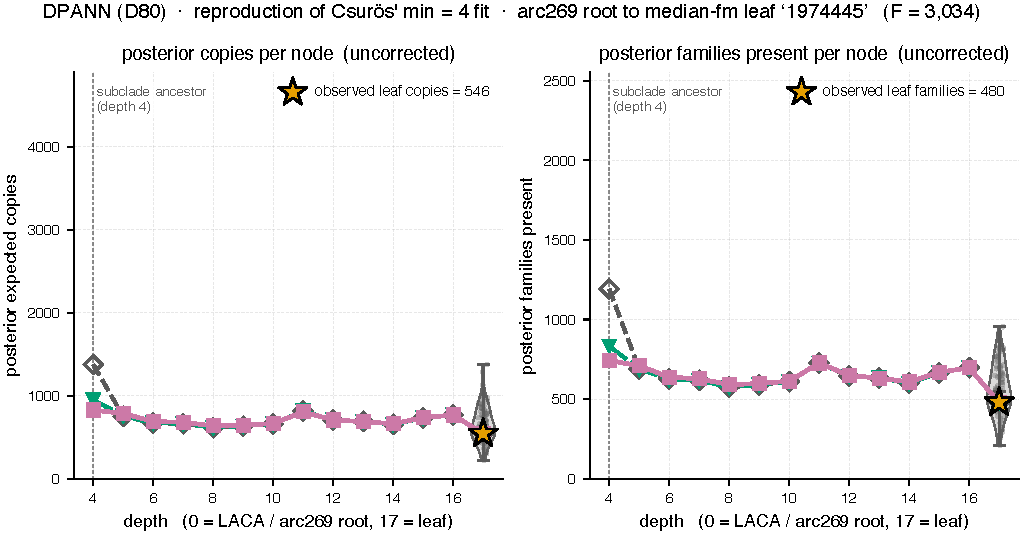
\includegraphics[width=0.92\linewidth,height=\textheight,keepaspectratio,alt={DPANN reproduction trajectory}]{../validation/outputs/subset_reproduction_path_dpann80.pdf}

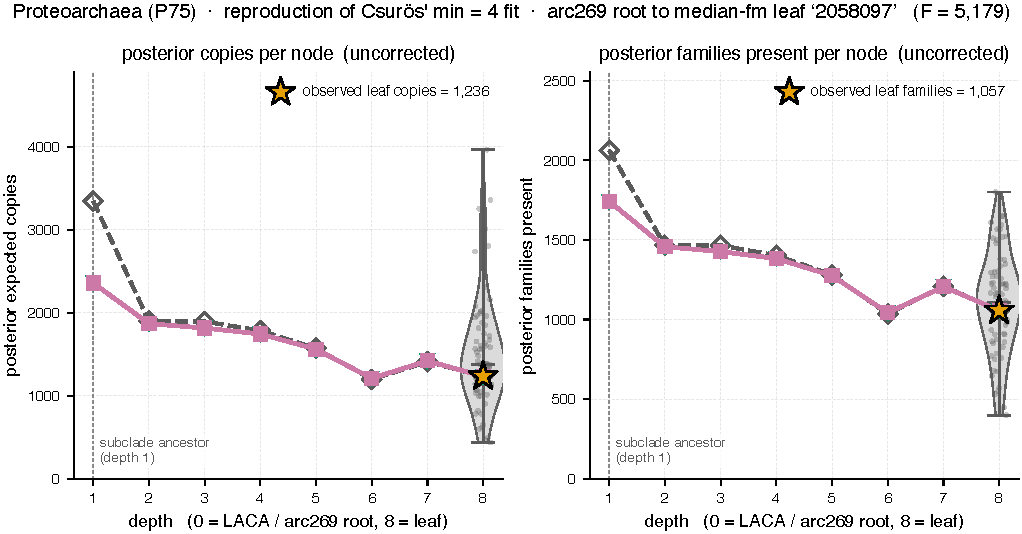
\includegraphics[width=0.92\linewidth,height=\textheight,keepaspectratio,alt={Proteoarchaea reproduction trajectory}]{../validation/outputs/subset_reproduction_path_proteo75.pdf}

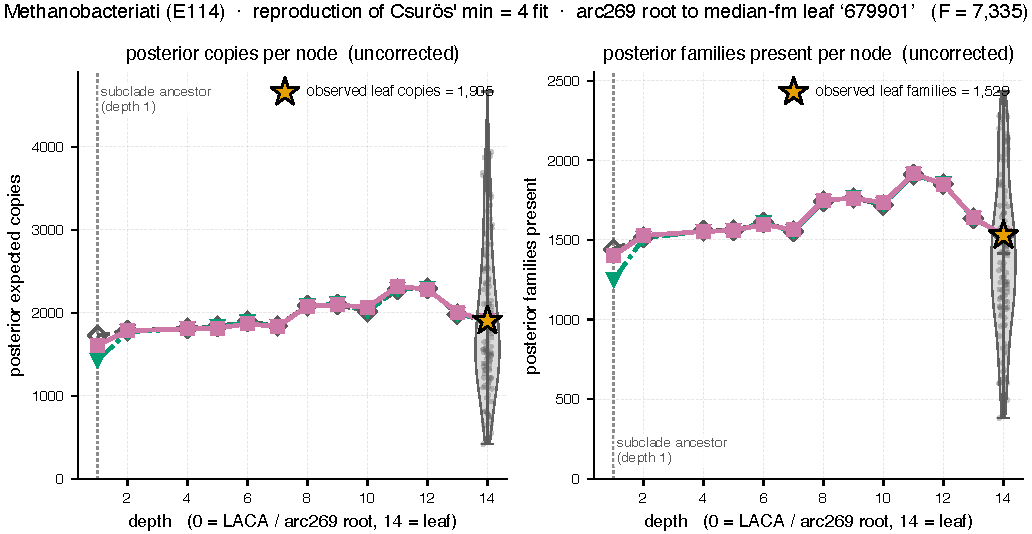
\includegraphics[width=0.92\linewidth,height=\textheight,keepaspectratio,alt={Methanobacteriati reproduction trajectory}]{../validation/outputs/subset_reproduction_path_eury114.pdf}

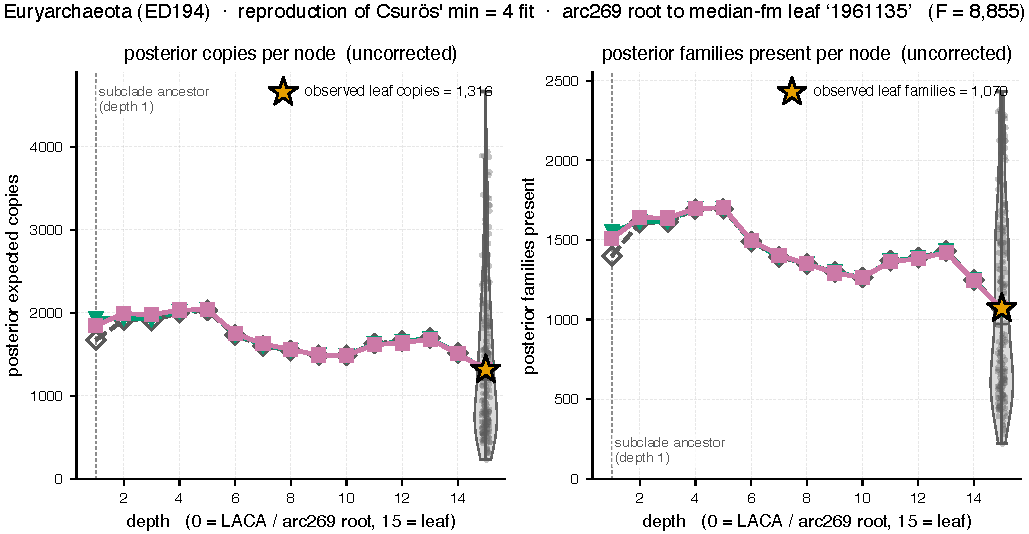
\includegraphics[width=0.92\linewidth,height=\textheight,keepaspectratio,alt={Euryarchaeota reproduction trajectory}]{../validation/outputs/subset_reproduction_path_ed194.pdf}

\textbf{Figure 1.} Per-subclade posterior reproduction trajectories from
the arc269 root to each subset's median-fm leaf, for Csurös' subset-only
ML and recount's two recommended fits.

Reading each panel of Figure 1: the three lines run from the arc269-root
depth (left) to the median-fm leaf depth (right), and all three meet the
OBSERVED gold-star value at the leaf tip on every subset. They diverge
at the deeper internal nodes, where the recommended modes (purple,
olive) sit close to Csurős' reference (gray dashed). The L(0)-amplified
counterparts are in \hyperref[l0-corrected-trajectories]{L(0)-corrected
trajectories}; both the panels and the shared legend are regenerated by
\texttt{validation/reproduction\_path\_plots.py}.

\subsection{Constraint regime}\label{constraint-regime}

Two complementary regularisers shape the fit; both default to \emph{on}.

\subsubsection{Sub-critical Yule cap on
duplication}\label{sub-critical-yule-cap-on-duplication}

Per-branch duplication is bounded \emph{just below} the loss rate via
the logit transform dup\_v = cap · sigmoid(θ\_v), where the cap
\texttt{MAX\_PROB\_NOT1} = 1 − 2⁻³⁰ ≈ 0.99999999907. Equivalently the
Pólya shape parameter κ\_v · (1 − q\_v) \textgreater{} 0 everywhere,
keeping the branching process sub-critical. This matches the
\texttt{is\_duprate\_bounded\ =\ true} default in Csurös' Java
(\href{https://github.com/miklosc/Count/blob/master/src/count/model/MLDistribution.java\#L157}{MLDistribution.java:157})
and the convention documented in \textbf{Csűrös 2026 PNAS} (full
citation in \hyperref[citing]{Citing}). Without the cap the optimizer
can let dup → ∞ on individual branches and the likelihood runs away
along a ridge of equally-good but biologically meaningless solutions;
see \url{NO_DUPLICATION_CONSTRAINT.md} for the unconstrained snapshot.

\subsubsection{Why a prior is a more general (and arguably more
biological)
choice}\label{why-a-prior-is-a-more-general-and-arguably-more-biological-choice}

Csurös' sub-critical cap is a \textbf{hard constraint} on a single
quantity (dup ≤ 1 per branch). It rules out the literal dup → ∞
pathology but leaves the rates on neighbouring branches
\textbf{statistically independent} --- adjacent edges of the same clade
can still take wildly different values, gain can still blow up to
\textasciitilde10¹⁴ at isolated nodes (\url{GAIN_CONSTRAINT.md} walks
the published-rate forensics), and the optimizer keeps finding multiple
local basins.

A \textbf{prior} is a more general regulariser and is arguably better
motivated biologically. The Brownian prior (mode 4 in the canonical
queue) places a Gaussian on the \textbf{log-rate increment} between
parent and child branches:

log r\_v − log r\_pa(v) \textasciitilde{} Normal(0, σ²·t\_v) for each
rate axis r ∈ \{γ, λ, t\}, each non-root v

This is the \textbf{Thorne--Kishino--Painter} autocorrelated-rate model
(Thorne, Kishino, Painter 1998, \emph{Estimating the rate of evolution
of the rate of molecular evolution}, MBE 15(12):1647--1657), originally
proposed for molecular-clock relaxation and reused here for GLD rate
variation. It captures a substantive biological assumption:
\textbf{rates of gene-content evolution are auto-correlated along the
tree} --- sister branches that share recent ancestry should have similar
rates a priori, because the biological mechanisms governing
gain/loss/duplication (genome size, lifestyle, mutational regime)
themselves vary smoothly along the species tree.

The mathematical specification and the bit-perfect FD-validated gradient
are in \url{docs/brownian_prior.pdf}. The 2026-05-19 update for arc269 +
subsets data:

\begin{itemize}
\tightlist
\item
  \textbf{All 5 subset Brownian fits sit inside the sub-critical region}
  without needing the dup-cap to be active --- the prior dominates and
  the cap is never reached. Max gain stays bounded at ≲ 10² (vs Csurös'
  published 5×10¹⁴).
\item
  \textbf{The Brownian prior subsumes the sub-critical cap as a special
  case}: in the σ → ∞ limit the prior is uniform and the cap is the only
  thing keeping dup bounded; for finite σ the prior softly penalises any
  large rate excursion long before it reaches the cap.
\end{itemize}

The cap is kept \emph{on by default} as a hard fallback for ML-only fits
(modes 1 and 2) where no prior is active. For MAP fits (modes 3, 4) the
cap is rarely binding.

\subsection{Does GLD give a sound foundation for ancestral genome
inference?}\label{does-gld-give-a-sound-foundation-for-ancestral-genome-inference}

Csurős 2026 PNAS closes its abstract with a claim: \emph{``The GLD
framework provides a statistically sound foundation for hypothesizing
about gene content evolution across the diversity of entire kingdoms.''}
The \hyperref[demonstration-of-reproduction]{reproduction section} above
confirms the first half --- the GLD likelihood, its gradient and the
Ωmin sampling-bias correction are implemented correctly, and the recount
fits recover Csurős' published rates to within a few nat of
log-likelihood. This section tests the second half: when GLD is used to
reconstruct an \emph{ancestral genome} from gene-copy-number data, is
the result a sound foundation for hypotheses about how gene content
evolved across a whole kingdom?

Tested on 269 archaeal genomes (arc269 --- a superset that contains
Csurős' four focal subset clades as slices), the answer is no. The
argument runs in three steps:

\begin{enumerate}
\def\labelenumi{\arabic{enumi}.}
\tightlist
\item
  \textbf{GLD cannot separate horizontal transfer from inheritance.} It
  reads only per-genome copy counts; two families with the same counts
  get the same likelihood whether they were inherited from a common
  ancestor or spread between lineages by transfer.
\item
  \textbf{Unfiltered, GLD fits the family-size data well --- and infers
  an ancestor larger than any living archaeon.} The inflation is the
  expected behaviour of a copy-number-only method on a kingdom with
  pervasive transfer; it is not a fitting failure, because the
  unfiltered fit is the \emph{best} fit to the family-size distribution.
\item
  \textbf{The family-size filter that suppresses the inflation has no
  GLD-internal justification, and it makes the fit to the family- size
  distribution worse.}
\end{enumerate}

Scope. We do not dispute the GLD likelihood or its algorithms --- the
reproduction section affirms both. The claim under test is the narrower,
downstream one: that a GLD fit to copy-number data is a sound
\emph{foundation for ancestral gene-content inference} across a kingdom.

\subsubsection{1 --- Copy numbers cannot separate transfer from
inheritance}\label{1--copy-numbers-cannot-separate-transfer-from-inheritance}

The GLD likelihood factors over gene families. For one family it reads a
single integer per genome --- how many copies of that family the genome
carries --- and nothing else. Call the family's vector of per-genome
copy counts its \emph{profile}, Ξ = (Ξ\_1, \ldots, Ξ\_N) over the N
leaves of the tree. The likelihood L(Ξ \textbar{} rates) is a function
of that integer vector and the tree; no other feature of the family
enters.

GLD is a likelihood model. For each family it does not choose a single
history; it sums over every history its model permits --- every
arrangement of gains, losses and duplications along the species-tree
branches --- weighting each by its probability under the fitted rates.
The posterior it reports for ``family present at node X'' is the
rate-weighted share of those histories in which the family is present at
X.

Two consequences follow. First, that posterior is a function of the
copy-number profile, the tree and the fitted rates, and of nothing else:
two families with identical profiles receive identical posteriors,
necessarily. Second, GLD's space of histories contains only vertical
events --- gain, loss, duplication along the tree. It has no
horizontal-transfer edge.

Now take a family found in clade A and clade C but not in the clade B
that lies between them. Its true history might be vertical --- present
in the A--B--C common ancestor, then lost on the lineage to B --- or
horizontal --- arisen within A, carried into C by transfer, never in the
A--B--C ancestor. The two produce the same copy-number profile. GLD,
scoring that profile, has no transfer history available. It accounts for
the profile with the gain--loss--duplication histories its model does
permit: a single gain in the A--B--C ancestor followed by a loss in B,
or two independent gains --- one in A, one in C --- with no copy ever in
the A--B--C ancestor. Only the first is a vertical history; the second
is not, but neither is it a transfer --- GLD's model has no edge that
carries a copy from one lineage to another. The relative weight of these
histories is set by the fitted rates: a rare gain rate with a high loss
rate favours the single-ancestral-gain history, the reverse favours the
independent-gain history. This is a likelihood, not a parsimony
reconstruction: GLD does not pick the ancestral history, it integrates
over all of them. But whatever ancestral posterior the integration
yields, GLD returns the \emph{same} value for the genuinely ancestral
family and for the transferred one --- their profiles are identical, and
the profile is the whole input.

\pandocbounded{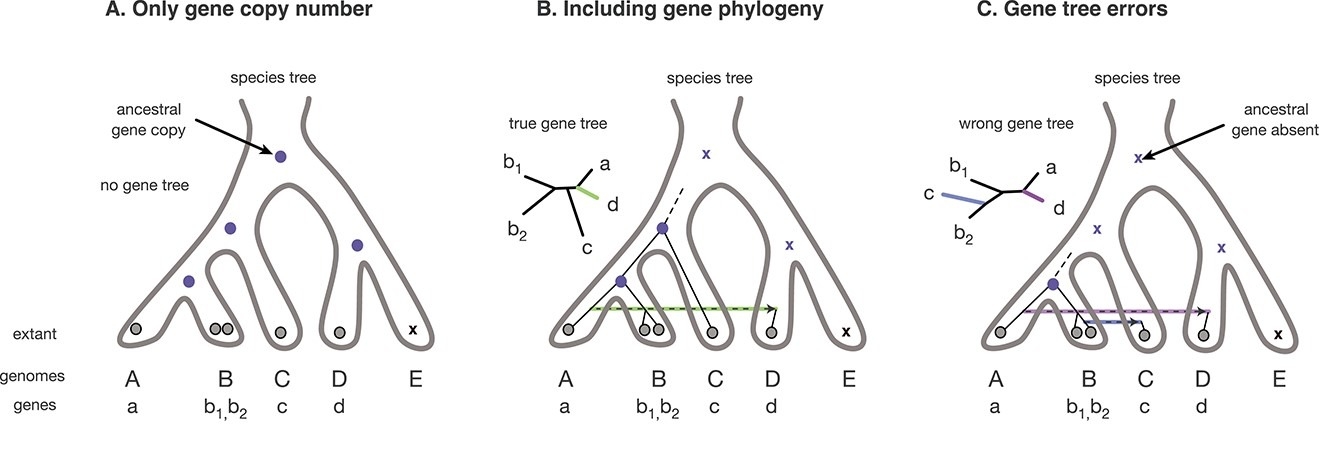
\includegraphics[keepaspectratio,alt={Gene-tree topology vs profile-only inference of transfer --- Williams 2024 Fig 2}]{figures/williams2024_reconciliation_fig2.jpeg}}

\textbf{Figure 2.} \emph{A sampled gene-tree topology distinguishes a
horizontally transferred gene family from a vertically inherited one ---
the distinction a copy-number profile alone cannot make. Reproduced
under fair use from T. A. Williams, A. A. Davin, L. L. Szánthó et al.,
``Phylogenetic reconciliation: making the most of genomes to understand
microbial ecology and evolution,'' The ISME Journal 18:wrae129 (2024).}

This is a structural property of copy-number-only inference, and it is
the reason gene-tree-reconciliation methods exist: a sampled gene-tree
topology \emph{does} carry information that separates a transferred
family from an inherited one, and reconciliation methods use it
(\href{https://doi.org/10.1093/ismejo/wrae129}{Williams, Davin, Szánthó
\emph{et al.} 2024}, Fig 2, reproduced above as Figure 2). GLD does not
consume gene trees, so it cannot make that separation.

\paragraph{A worked example}\label{a-worked-example}

A small tree that shows the problem has five genomes, related as
(((A,B),C),(D,E)). One gene family is present in A (one copy), B (two
copies), C (one) and D (one), and absent in E. The unrooted gene tree of
the five gene copies is ((a,d),(b1,b2),c): the copy in A and the copy in
D are each other's closest relatives. A and D are distant in the species
tree --- A inside the ABC clade, D in the DE clade --- so the a--d
pairing is discordant with the species tree: the transfer signature
Figure 2 illustrates. Reading that gene tree, reconciliation recovers
the family's true history --- it originates on the branch leading to the
ABC ancestor, one copy is transferred from the A lineage to D, and one
copy duplicates on the terminal branch to B. The family is genuinely
present at A, AB, ABC and D; the root (the ABCDE ancestor), the DE
ancestor and E are empty of it.

GLD sees none of the gene tree; it has only the copy-number profile
{[}A=1, B=2, C=1, D=1, E=0{]}. Reconstructed in recount with global
rates and unit branch lengths, GLD's posterior probability that the
family is present (≥ 1 copy) at each node along the two root-ward
trajectories --- D → DE → root and A → AB → ABC → root --- is a function
of the global gain rate. The plots below (Figure 3) trace it at two
fixed loss rates (loss is the GLD time unit; the duplication rate is
held at 0.2). The dotted black line is the true history --- present at
A, AB, ABC and D, absent at DE and the root.

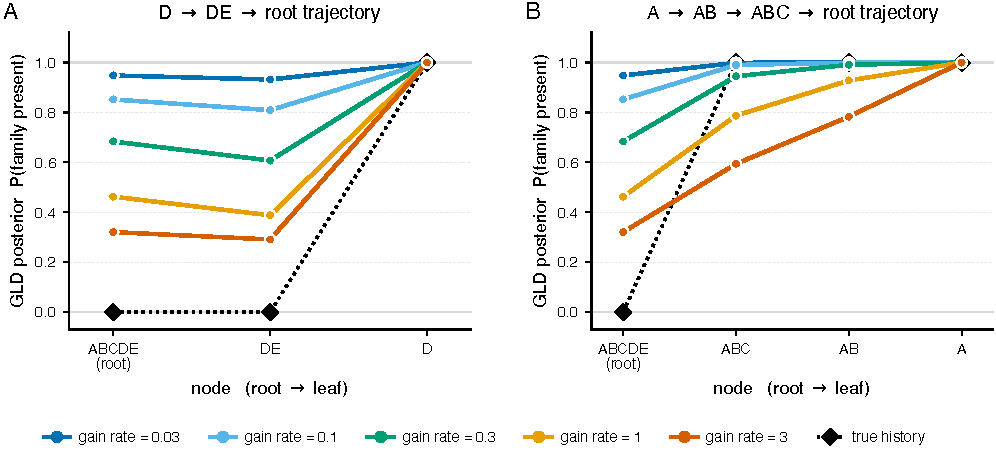
\includegraphics[width=0.92\linewidth,height=\textheight,keepaspectratio,alt={GLD presence posterior along the two root-ward trajectories at loss rate 1, one curve per global gain rate, with the true history dotted}]{../validation/outputs/transfer_traj_loss1.pdf}

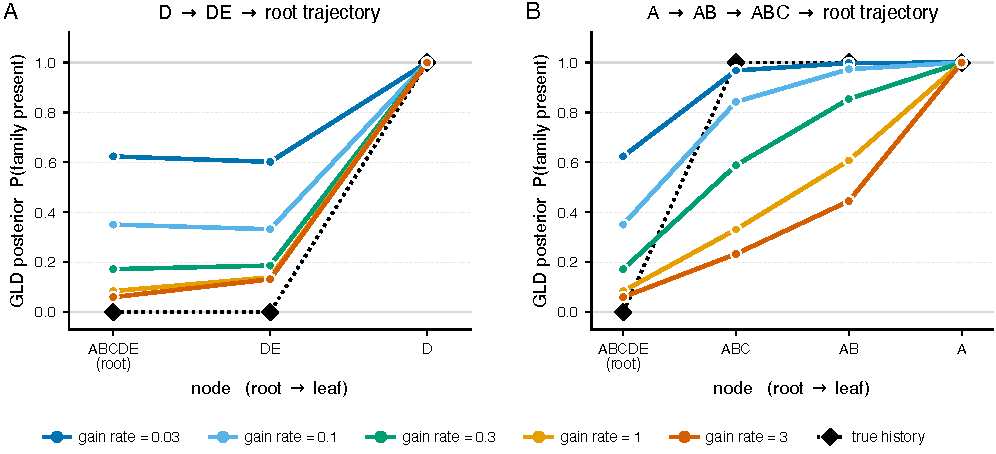
\includegraphics[width=0.92\linewidth,height=\textheight,keepaspectratio,alt={The same trajectories at loss rate 2}]{../validation/outputs/transfer_traj_loss2.pdf}

\textbf{Figure 3.} GLD presence posterior along the two root-ward
trajectories of the worked example, at loss rates 1 and 2, one curve per
global gain rate, with the true history dotted.

Read each trajectory from the root (left) to the leaf (right). On D → DE
→ root the true history places the family only at the leaf D, yet GLD
lifts DE and the root well above the dotted zero line --- at loss rate
1, DE to 0.29--0.93 and the root to 0.32--0.95 over the gain rates
shown, lower at loss rate 2 but still positive. D's copy, a transfer, is
read by the copy-number likelihood as evidence for the family deep in
the tree. On A → AB → ABC → root GLD keeps the family through ABC, the
clade it truly arose in, then carries it on to the root --- empty in the
true history --- by the same amount. The spurious ancestral mass shrinks
as the gain rate rises (independent gains become cheap) and as the loss
rate rises, but it never reaches zero, the true value.

Which positive number GLD reports is set by the rates --- and the rates
are not a per-family quantity. GLD estimates one set of rates jointly
from the entire dataset, and those dataset-level rates then shape every
individual family's reconstructed history. That much it shares with
phylogenetic reconciliation methods, which likewise estimate their
parameters across the whole dataset and apply them family by family. The
difference is the information each family contributes: a reconciliation
method also reads that family's gene tree, recovered from its sequence
alignment, and the alignment carries the signal that separates a
transfer from an inheritance. GLD reads only the family's copy numbers,
which do not carry that signal. The trajectory computations are
reproduced by \url{validation/transfer_identifiability_example.py}.

This biases ancestral inference in a definite direction. A copy acquired
by transfer sits in a clade the family never reached by descent; GLD,
having no transfer edge, can join it to the rest of the family only
through a common ancestor in the species tree --- a node deeper than the
family's true origin. In the worked example the family arose in the ABC
clade, but its transferred copy in D forces GLD to seat the family at
the root, the common ancestor of the ABC clade and D, where the family
never was. Its correct contribution to that root is zero; GLD gives it a
positive one --- the posterior its profile earns, the same a genuinely
root-ancestral family with that profile would get. Each cross-clade
transferred family therefore adds spurious mass to the ancestral count,
and the bias has a sign: transfer can only push the inferred ancestor
\emph{upward}. Archaea, like other prokaryotes, exchange genes by
horizontal transfer extensively --- resolving transfer is the problem
the reconciliation literature is built around --- so on archaeal data
this upward bias is not an edge case. Its magnitude cannot be read off
the copy numbers, because the copy numbers cannot say which families
were transferred; section 2 measures the inferred ancestor that results.

\subsubsection{2 --- Unfiltered GLD: a good fit to family sizes, an
ancestor larger than any living
archaeon}\label{2--unfiltered-gld-a-good-fit-to-family-sizes-an-ancestor-larger-than-any-living-archaeon}

This section makes two observations about the unfiltered fit (every
family with at least one copy somewhere; no family-size filter). They
pull in opposite directions, and that tension is the point:

\begin{itemize}
\tightlist
\item
  the unfiltered fit \textbf{reproduces the empirical distribution of
  family sizes} --- it is the only fit in the whole filter sweep that
  does;
\item
  the same fit \textbf{infers an ancestor with more gene families than
  the richest modern archaeal genome in the data} carries.
\end{itemize}

The unfiltered fit is not a failed fit that a better optimiser would
cure: it already reproduces the family-size distribution (below). The
inflation is therefore not an optimisation artefact --- it is intrinsic
to reconstructing ancestry from copy numbers (section 1).

\paragraph{What the GLD likelihood predicts about family
sizes}\label{what-the-gld-likelihood-predicts-about-family-sizes}

Under the fitted GLD birth-death process every family has a random
profile Ξ; let Ω(Ξ) = Σ\_v Ξ\_v be its \emph{total copy count} summed
over all leaves. The process induces a distribution over Ω. Define

L(0, N) = P( Ω(Ξ) \textless{} N \textbar{} fitted γ, λ, μ, t )

--- the model's own predicted fraction of families whose total copy
count falls below N. (Csurős writes this L(0); it is the sampling-bias
term --- the mass the rate process puts on families too small to be seen
once a sum ≥ Ωmin filter is applied.)

The numerical value of L(0, N) is tied to the evaluation universe: the
same fitted rates can give different L(0, N) values when Ω is computed
over the fit's own training leaves/filter universe versus over the full
arc269 leaf set used for the histogram check below.

Two quantities follow:

\begin{itemize}
\tightlist
\item
  the per-bin probability P(Ω = k) = L(0, k+1) − L(0, k);
\item
  the implied total family count F* = F / (1 − L(0, Ωmin)), where F is
  the number of families the fit actually sees --- the Csurős
  extinction-amplification that scales observed ancestral counts back up
  for families that left no trace.
\end{itemize}

If the fitted rates describe the family-size distribution over the
evaluation universe, the predicted counts F* · P(Ω = k) should match the
empirical number of families with total copy count k --- both above the
filter, where the fit was trained, and below it, where the underlying
profile still records the small families the filter discarded. The next
subsection runs exactly that check.

This comparison is a posterior-predictive check, written in closed form.
The identity F* · (1 − L(0, Ωmin)) = F is only the normalisation implied
by the observation filter; it is not the test. The test is the bin-wise
comparison F* · P(Ω = k) versus the empirical histogram. F* · P(Ω = k)
is the expected count of families with total copy count k that one would
obtain by simulating F* families from the fitted GLD process and
tallying them by size; the Pn-tensor recursion (Csurős SI Theorems 3--5)
returns that expectation directly, so the test carries no Monte-Carlo
noise. The question it asks is the standard one for any fitted
generative model: draw gene families from it, and do you recover the
family-size distribution that was actually observed? (It is a
\emph{plug-in} predictive check --- it uses the point-estimate rates;
for fits over tens of thousands of families the rate uncertainty is
negligible next to the discrepancies seen below.)

As a sanity check on the L(0) bin calculation itself,
\url{validation/pnas_l0_family_size_sim.py} forward-simulates raw
families from the two rate sets used in the PNAS letter figure and
compares the simulated Ω bins with L(0,k+1)−L(0,k). With 250,000 raw
simulated families per fit, the Ω ≥ 2 conditional simulated/predicted
ratios are 0.972--1.025 for the unfiltered fit and 0.987--1.009 for the
Ωmin=4 fit
(\href{validation/results/pnas_l0_family_size_sim.json}{JSON};
\href{validation/results/pnas_l0_family_size_sim.png}{ratio plot};
\href{validation/results/pnas_l0_family_size_sim_loglog.png}{log-log
plot}).

\paragraph{Goodness-of-fit: empirical vs model-predicted family-size
histogram}\label{goodness-of-fit-empirical-vs-model-predicted-family-size-histogram}

Empirical arc269 sum-bin histogram (full F = 90,243). Every family has
total copy count Ω ≥ 1: a family with Ω = 0 is present in no genome,
leaves no trace, and so is unobservable in principle --- the Ω = 0 bin
is empty in any dataset, not only this one. The rate process, by
contrast, does assign Ω = 0 a probability (the sampling-bias term L(0,
1)); that predicted-but-unobservable mass is what the goodness-of-fit
test below has to handle separately from the observed bins:

\textbf{Table 6.} Empirical arc269 sum-bin family-size histogram over
the full F = 90,243 families.

\begin{center}
\begin{adjustbox}{max width=\textwidth}
\begin{tabular}{@{}rrr@{}}
\toprule\noalign{}
sum k & empirical count & \% of arc269 \\
\midrule\noalign{}
1 (singleton) & 65,339 & 72.40 \\
2 & 9,491 & 10.52 \\
3 & 3,859 & 4.28 \\
4 & 2,062 & 2.28 \\
5 & 1,176 & 1.30 \\
6 & 851 & 0.94 \\
7 & 644 & 0.71 \\
≥ 8 & 6,821 & 7.57 \\
\bottomrule\noalign{}
\end{tabular}
\end{adjustbox}
\end{center}

\textbf{Unconditional test:} predicted F* · P(Ω = k) divided by
empirical E(k). 1 = perfect; \textless{} 1 = model under-predicts;
\textgreater{} 1 = over-predicts. Rows are sequential arc269 fits at
increasing filter strength.

\textbf{Table 7.} Unconditional goodness-of-fit --- predicted/empirical
family-size ratio per sum bin, one row per arc269 fit.

\begin{center}
\begin{adjustbox}{max width=\textwidth}
\begin{tabular}{@{}lrrrrrrrr@{}}
\toprule\noalign{}
fit (filter, L(0,Ωmin)) & k=1 & k=2 & k=3 & k=4 & k=5 & k=6 & k=7 & sum
≥ 8 \\
\midrule\noalign{}
\textbf{mc=1 no filter} (L(0,1) = 0.79) & \textbf{0.94} & \textbf{1.29}
& \textbf{1.11} & \textbf{1.03} & \textbf{1.09} & \textbf{1.06} &
\textbf{1.08} & \textbf{1.08} \\
sum ≥ 2 (L(0,2) = 0.40) & 0.10 & 0.46 & 0.84 & 1.17 & 1.56 & 1.68 & 1.80
& 1.54 \\
sum ≥ 3 (L(0,3) = 0.27) & 0.03 & 0.17 & 0.35 & 0.57 & 0.86 & 1.04 & 1.22
& 1.50 \\
sum ≥ 4 (Csurös) (L(0,4) = 0.21) & 0.01 & 0.09 & 0.19 & 0.32 & 0.51 &
0.65 & 0.79 & 1.35 \\
sum ≥ 5 (L(0,5) = 0.18) & 0.01 & 0.05 & 0.13 & 0.21 & 0.34 & 0.45 & 0.56
& 1.22 \\
sum ≥ 6 (L(0,6) = 0.17) & 0.00 & 0.04 & 0.09 & 0.16 & 0.26 & 0.34 & 0.43
& 1.14 \\
sum ≥ 7 (L(0,7) = 0.16) & 0.00 & 0.02 & 0.07 & 0.12 & 0.21 & 0.28 & 0.35
& 1.06 \\
sum ≥ 8 (L(0,8) = 0.16) & 0.00 & 0.02 & 0.05 & 0.10 & 0.17 & 0.23 & 0.29
& 1.00 \\
sum ≥ 9 (L(0,9) = 0.15) & 0.00 & 0.01 & 0.04 & 0.08 & 0.14 & 0.19 & 0.25
& 0.95 \\
sum ≥ 10 (L(0,10) = 0.15) & 0.00 & 0.01 & 0.03 & 0.06 & 0.11 & 0.16 &
0.21 & 0.90 \\
union-min4 (L(0,4) = 0.21) & 0.01 & 0.08 & 0.18 & 0.29 & 0.47 & 0.60 &
0.74 & 1.32 \\
\bottomrule\noalign{}
\end{tabular}
\end{adjustbox}
\end{center}

(The L(0,Ωmin) values in this table are computed with
\texttt{unobserved\_logL0\_native} over the full 269-leaf arc269
evaluation universe. They are therefore goodness-of-fit quantities for
the full arc269 sum-bin histogram, not necessarily the same L(0,Ωmin)
values used internally by a fit under its own training filter. For
example, the union-min4 fit reports a much smaller training-filter
correction for its own union family set, whereas its full-arc269
histogram check gives L(0,4) = 0.21.)

\textbf{Two objections to the unconditional comparison, and what the
conditional tests handle.} The unconditional ratio mixes two issues.
First, the unfiltered fit's apparent advantage on the full histogram is
partly tautological --- the mc = 1 likelihood was trained on every bin
including the singletons, so it has a built-in advantage there over any
filtered fit that never saw k \textless{} Ωmin. Second, the singleton
stratum itself (Ω = 1, 72 \% of arc269) is the bin a birth-death model
is most open to doubt on: a gene called in a single genome may be a very
recent arrival, or an annotation artefact, rather than a family with the
kind of gain / loss / duplication history GLD describes. A fair reading
might be that the filtered fits fail only because of one or both of
these effects, and would be fine on the families that matter.

The two conditional tests below remove both objections at once. Each
re-runs the comparison with the smallest families dropped from both the
model and the data --- singletons for the Ω ≥ 2 test, singletons plus
2-copy families for the Ω ≥ 3 test --- and re-normalises the model's
predicted distribution to the same range, so predicted and empirical
mass are conserved on the bins both fits speak to. On those bins neither
fit has a training-set advantage, and a shape divergence is a genuine
fit-quality difference rather than an artefact of which strata each fit
was trained on.

\textbf{Conditioned on Ω ≥ 2} (singletons excluded):

\textbf{Table 8.} Conditional goodness-of-fit with singletons excluded
--- predicted/empirical ratio per sum bin, re-normalised over Ω ≥ 2.

\begin{center}
\begin{adjustbox}{max width=\textwidth}
\begin{tabular}{@{}lrrrrrrr@{}}
\toprule\noalign{}
fit (filter, L(0,Ωmin)) & k=2 & k=3 & k=4 & k=5 & k=6 & k=7 & sum ≥ 8 \\
\midrule\noalign{}
\textbf{mc=1 no filter} & \textbf{1.11} & \textbf{0.96} & \textbf{0.89}
& \textbf{0.94} & \textbf{0.91} & \textbf{0.93} & \textbf{0.93} \\
sum ≥ 2 & 0.46 & 0.84 & 1.17 & 1.56 & 1.68 & 1.80 & 1.54 \\
sum ≥ 3 & 0.25 & 0.51 & 0.83 & 1.26 & 1.52 & 1.78 & 2.19 \\
sum ≥ 4 (Csurös) & 0.17 & 0.37 & 0.61 & 0.97 & 1.23 & 1.51 & 2.56 \\
sum ≥ 5 & 0.12 & 0.28 & 0.49 & 0.79 & 1.01 & 1.27 & 2.79 \\
sum ≥ 6 & 0.09 & 0.23 & 0.41 & 0.68 & 0.88 & 1.11 & 2.94 \\
sum ≥ 7 & 0.07 & 0.19 & 0.35 & 0.60 & 0.79 & 1.00 & 3.05 \\
sum ≥ 8 & 0.05 & 0.15 & 0.30 & 0.53 & 0.71 & 0.91 & 3.13 \\
sum ≥ 9 & 0.04 & 0.13 & 0.26 & 0.47 & 0.65 & 0.84 & 3.20 \\
sum ≥ 10 & 0.03 & 0.10 & 0.22 & 0.41 & 0.58 & 0.76 & 3.27 \\
union-min4 & 0.16 & 0.35 & 0.58 & 0.93 & 1.18 & 1.46 & 2.61 \\
\bottomrule\noalign{}
\end{tabular}
\end{adjustbox}
\end{center}

\textbf{Conditioned on Ω ≥ 3} (1+2-copy families excluded as well):

\textbf{Table 9.} Conditional goodness-of-fit with 1- and 2-copy
families excluded --- predicted/empirical ratio per sum bin,
re-normalised over Ω ≥ 3.

\begin{center}
\begin{adjustbox}{max width=\textwidth}
\begin{tabular}{@{}lrrrrrr@{}}
\toprule\noalign{}
fit (filter, L(0,Ωmin)) & k=3 & k=4 & k=5 & k=6 & k=7 & sum ≥ 8 \\
\midrule\noalign{}
\textbf{mc=1 no filter} & \textbf{1.03} & \textbf{0.95} & \textbf{1.01}
& \textbf{0.98} & \textbf{0.99} & \textbf{1.00} \\
sum ≥ 2 & 0.63 & 0.88 & 1.17 & 1.26 & 1.35 & 1.15 \\
sum ≥ 3 & 0.35 & 0.57 & 0.86 & 1.04 & 1.22 & 1.50 \\
sum ≥ 4 (Csurös) & 0.24 & 0.40 & 0.64 & 0.81 & 1.00 & 1.70 \\
sum ≥ 5 & 0.18 & 0.31 & 0.51 & 0.66 & 0.82 & 1.81 \\
sum ≥ 6 & 0.15 & 0.27 & 0.44 & 0.57 & 0.71 & 1.88 \\
sum ≥ 7 & 0.12 & 0.22 & 0.38 & 0.50 & 0.63 & 1.94 \\
sum ≥ 8 & 0.10 & 0.19 & 0.34 & 0.45 & 0.57 & 1.98 \\
sum ≥ 9 & 0.08 & 0.16 & 0.30 & 0.41 & 0.52 & 2.01 \\
sum ≥ 10 & 0.06 & 0.14 & 0.26 & 0.36 & 0.48 & 2.05 \\
union-min4 & 0.23 & 0.38 & 0.61 & 0.78 & 0.96 & 1.72 \\
\bottomrule\noalign{}
\end{tabular}
\end{adjustbox}
\end{center}

\textbf{Visual summary} (five representative fits, three conditioning
modes side-by-side; log-y; horizontal dashed line at ratio = 1; green
band marks ``within 2×'' of perfect):

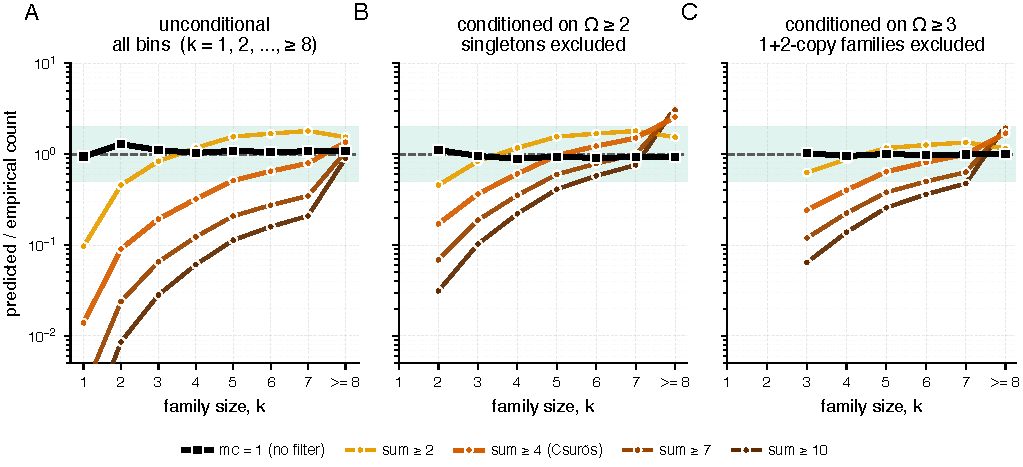
\includegraphics[width=0.92\linewidth,height=\textheight,keepaspectratio,alt={L(0) goodness-of-fit panels: predicted/empirical ratio vs sum bin, 5 fits × 3 conditioning modes}]{../validation/outputs/l0_gof_ratio_panels.pdf}

\textbf{Figure 4.} L(0) goodness-of-fit --- predicted/empirical
family-size ratio vs sum bin for five representative fits across three
conditioning modes.

Generated by \texttt{validation/l0\_gof\_plot.py} from the same fits
used by Tables 7--9. The mc=1 line (black squares) hugs the perfect-fit
line in every panel; the filtered fits (warm-color gradient on filter
strength) start far below 1 at low k and cross above 1 at high k ---
shape mismatch persists across all three conditioning modes.

\textbf{Focused view: mc = 1 reference vs canonical min = 4 fits} ---
predicted F* · P(Ω = k) vs empirical E(k) absolute counts at every sum
bin. In Figure 5, panel A is the mc = 1 reference (the fit that matches
the data); panels B and C are the canonical Ωmin = 4 fits (Csurös'
full-tree filter and the union-min4 filter):

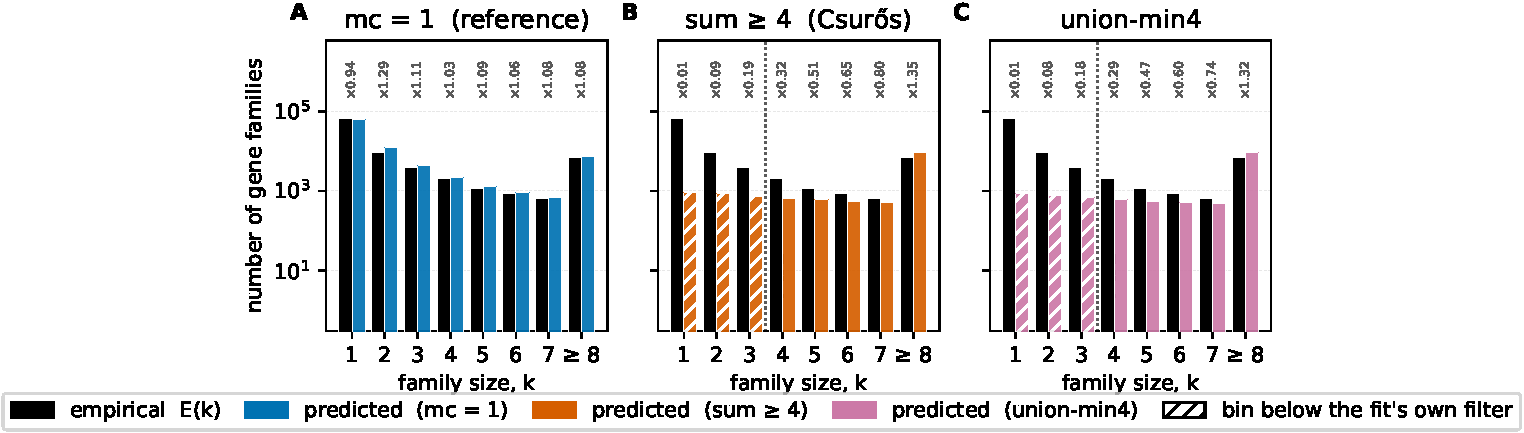
\includegraphics[width=0.92\linewidth,height=\textheight,keepaspectratio,alt={Focused min=4 GoF, with mc=1 reference: predicted vs empirical bars per sum bin, 3 fits}]{../validation/outputs/l0_gof_min4_focus.pdf}

\textbf{Figure 5.} Focused min = 4 goodness-of-fit --- predicted vs
empirical family counts per sum bin for the mc = 1 reference and the two
canonical Ωmin = 4 fits.

The same three panels with the bin axis extended to k = 30, so the
long-tail behaviour is visible family-size by family-size:

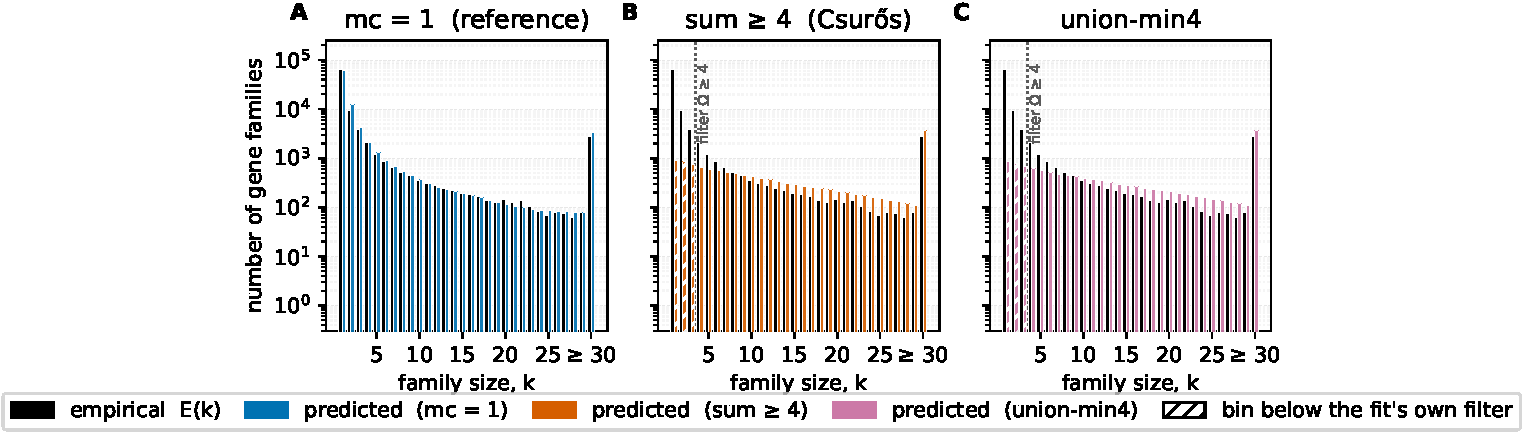
\includegraphics[width=0.92\linewidth,height=\textheight,keepaspectratio,alt={Focused min=4 GoF, tail view to k=30: predicted vs empirical bars per sum bin, 3 fits}]{../validation/outputs/l0_gof_min4_focus_k30.pdf}

\textbf{Figure 6.} The Figure 5 comparison with the bin axis extended to
k = 30, exposing the long-tail behaviour family-size by family-size.

Both generated by \texttt{validation/l0\_gof\_min4\_focus.py}; numeric
table (k = 1..7, ≥ 8) in \url{validation/outputs/l0_gof_min4_focus.txt}.
Figure 5 panel A is the reference: at mc = 1 every bar pair has ratio ≈
1.0 (0.94, 1.29, 1.11, 1.03, 1.09, 1.06, 1.08, 1.08). Figure 5 panels B
and C show the canonical filter-4 fits failing the same bins by 0.01 --
0.32 at sub-filter k \textless{} 4 (hatched) and 0.32 -- 0.80 just above
the filter. The contrast between ``what a fit that matches the data
looks like'' (Figure 5 panel A) and ``what the canonical Ωmin = 4 fits
actually produce'' (Figure 5 panels B and C) is the focal observation.

\textbf{Log-log version --- what the metric actually compares.} The
ratio test divides two count histograms; here are the two histograms
themselves on log-log, side by side, for the two filter-4 fits + the
mc=1 reference:

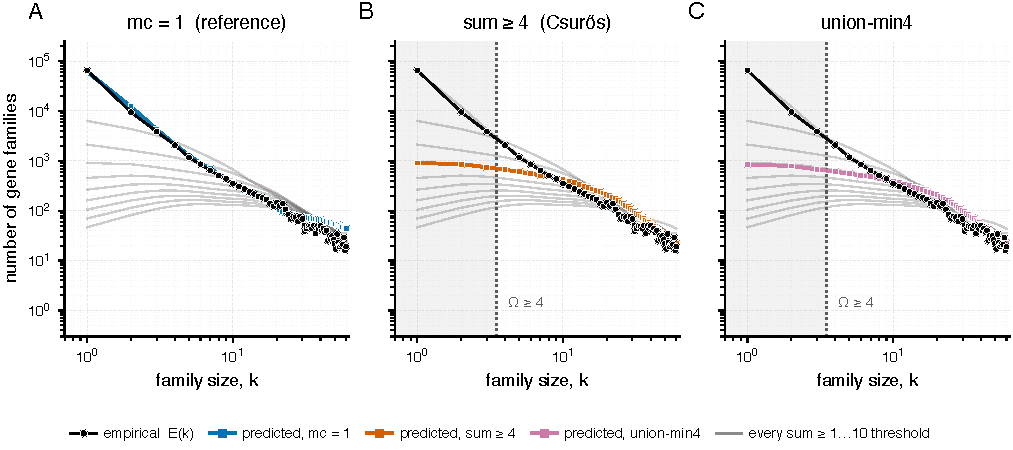
\includegraphics[width=0.92\linewidth,height=\textheight,keepaspectratio,alt={Sum-bin count histograms on log-log: predicted F* P(Ω=k) vs empirical E(k), 3 fits, mc=1 reference first}]{../validation/outputs/l0_gof_loglog.pdf}

\textbf{Figure 7.} Log-log sum-bin count histograms --- predicted F* ·
P(Ω = k) vs empirical E(k) for the mc = 1 reference and the two filter-4
fits.

Generated by \texttt{validation/l0\_gof\_loglog.py}. On log-log the
empirical histogram traces a power-law-like decay from sum=1 (65k
families) down to the tail at sum ≈ 60 (\textasciitilde10 families).
\textbf{Figure 7 panel A (mc=1, reference):} predicted curve (green
squares) overlays empirical across the entire range --- what a
well-described rate process looks like. \textbf{Figure 7 panels B and C
(sum ≥ 4 Csurös + union-min4):} predicted curves match empirical only
past k ≈ 5 and visibly diverge in the sub-filter region (k \textless{}
4, shaded gray) by 1--2 orders of magnitude.

\textbf{Reading Tables 7--9.} One fit reproduces the empirical
family-size histogram: the unfiltered \texttt{mc\ =\ 1} fit. Its
predicted/empirical ratio stays in \textbf{0.94--1.29} across every bin
unconditionally, and the two conditional tests confirm this is not an
artefact of the dominant singleton bin --- re-normalised to Ω ≥ 2
(singletons dropped) the ratios are \textbf{0.89--1.11}, and to Ω ≥ 3
(1- and 2-copy families dropped) \textbf{0.95--1.03}. To within roughly
10--30 \% per bin, the rate process the unfiltered fit recovers is a
good generative description of the marginal arc269 family-size
distribution.

\textbf{No filtered fit does this.} Every filtered sum ≥ N row of Tables
7--9 departs from the family-size histogram, and the departure grows
with the threshold N --- under-predicting the small families,
over-predicting the large-family tail. The conditional tests show this
is not a singleton artefact either: at sum ≥ 4 the Ω ≥ 2 ratios already
span 0.17--2.56. Section 3 returns to these rows; here they establish
only that the \emph{unfiltered} fit is the one fit in the sweep that
reproduces the family-size distribution.

A caution on the word ``fit''. That the unfiltered rate process
reproduces the family-\emph{size} distribution does not make its
\emph{ancestral} reconstruction correct. The size distribution is a
marginal --- one integer per family, pooled across families. The
ancestral reconstruction is a per-family, per-node claim, and section 1
showed it is not identifiable from copy numbers when transfer is
present. A perfectly calibrated generative model of family sizes can
still place every transferred family on the root. The good fit
established here matters for one reason: it removes ``the optimiser
failed'' as an explanation for what the rest of section 2 shows.

(Implementation note: L(0) and the Csurős F · L(0)/(1−L(0))
extinction-amplification reproduce bit-for-bit against Csurős' Java at
Ωmin \textgreater{} 1. At Ωmin = 1 the Pn-tensor pipeline is not wired
to the all-zeros branch, so the multiplicative ×1/(1−L(0)) form is
applied at internal nodes only. The three goodness-of-fit tables (Tables
7--9) are regenerated by \texttt{validation/l0\_goodness\_of\_fit.py};
the formal derivation of the unconditional and conditional histogram
checks is \url{docs/l0_conditional_gof.pdf}.)

\paragraph{\ldots and infers an ancestor larger than any living
archaeon}\label{and-infers-an-ancestor-larger-than-any-living-archaeon}

The same unfiltered \texttt{mc\ =\ 1} fit --- the one fit that
reproduces the family-size distribution --- places the arc269 root
(LACA, the last archaeal common ancestor) at \textbf{3,847 gene
families} (raw posterior). The richest single modern archaeal genome in
the data carries about \textbf{3,425} families: the unfiltered fit's
ancestor is larger than any genome alive today. Csurős' own
extinction-amplification --- multiplying by 1/(1 − L(0)) to restore
families that left no surviving copy --- uses L(0) = 0.79 here and lifts
the root estimate to \textbf{18,647 families}, roughly five times the
richest modern archaeon and an order of magnitude above the median
modern genome (≈ 890--1,642 families).

The same pattern holds clade by clade. Evaluated at each of the four
focal subclades' last common ancestors, the unfiltered arc269 fit infers
more families than the richest modern member of that subclade:

\textbf{Table 10.} Unfiltered arc269 fit at each subclade LCA, against
the richest and median modern genome below it.

\begin{center}
\begin{adjustbox}{max width=\textwidth}
\begin{tabular}{@{}lrrrr@{}}
\toprule\noalign{}
subclade & arc269 fit at the subclade LCA & richest modern genome below
it & median modern genome & LCA / median \\
\midrule\noalign{}
DPANN & 2,822 & 1,731 & 890 & 3.2 \\
Proteoarchaea & 3,565 & 3,425 & 1,419 & 2.5 \\
Methanobacteriati & 3,777 & 3,000 & 1,642 & 2.3 \\
Euryarchaeota & 3,777 & 3,000 & 1,284 & 2.9 \\
\bottomrule\noalign{}
\end{tabular}
\end{adjustbox}
\end{center}

(Family counts over the full F = 90,243 family universe; the ``arc269
fit'' column is the no-filter \texttt{mc\ =\ 1} posterior read at the
subclade's LCA node. Fitting each subclade on its own genomes instead
gives the same picture --- 1,732--3,666 families at the subclade root.)

This is the inflation. Section 1 gave the mechanism: every cross-clade
transferred family contributes ancestral posterior it should not, and
GLD has no way to discount it, so a copy-number fit on a transfer-rich
kingdom carries a systematic upward bias on ancestral content. From copy
numbers we cannot measure how much of the 3,847 is genuine ancestral
content and how much is that bias --- the identifiability gap of section
1 --- so the figure cannot be read as an ancestral genome size. The next
subsection asks whether the inflation is itself a modelling error; it is
not, which is exactly why it cannot be waved away.

The trajectory plots below (Figure 8) trace this node by node. Each
panel follows the path from the arc269 root to one subclade's median-fm
leaf; the red line is the unfiltered arc269 fit, the blue lines the
subclade fitted on its own genomes (also unfiltered). The gold star
marks the observed gene content of the leaf genome and the khaki violin
the spread across the subclade's other genomes --- the modern values the
reconstruction runs down to. In every subclade the fitted ancestor at
the root (left edge) stands well above the cloud of observed modern
genomes at the leaf (right edge).

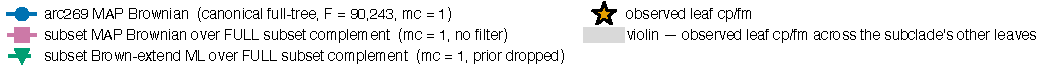
\includegraphics[width=0.92\linewidth,height=\textheight,keepaspectratio,alt={no-filter root-to-leaf path --- legend}]{../validation/outputs/min1_path_legend.pdf}

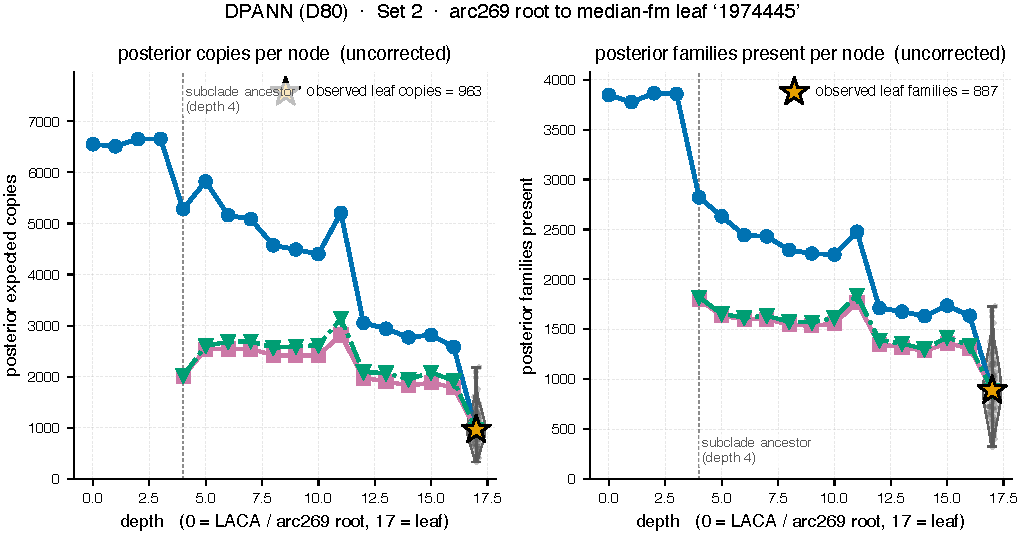
\includegraphics[width=0.92\linewidth,height=\textheight,keepaspectratio,alt={DPANN no-filter root-to-leaf path}]{../validation/outputs/min1_path_dpann80.pdf}

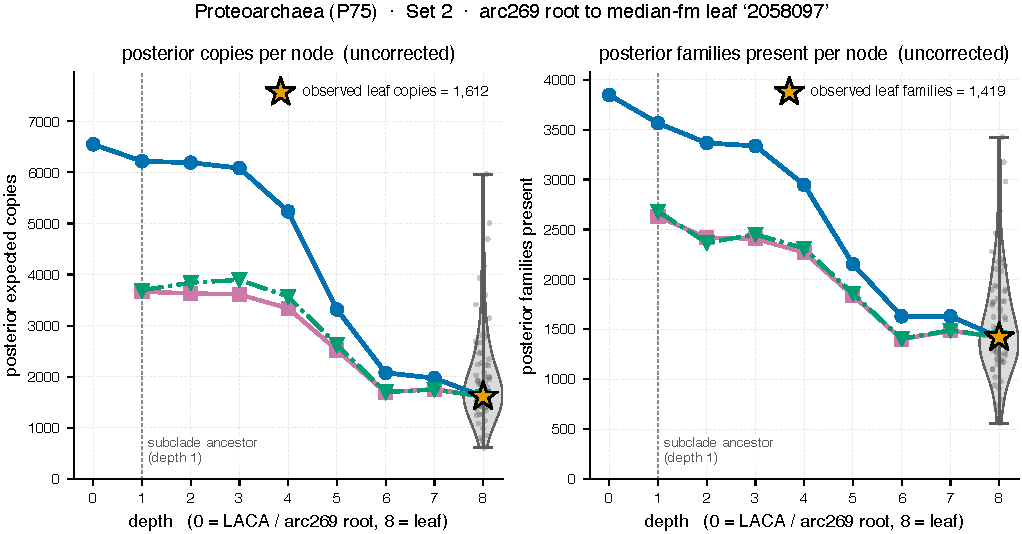
\includegraphics[width=0.92\linewidth,height=\textheight,keepaspectratio,alt={Proteoarchaea no-filter root-to-leaf path}]{../validation/outputs/min1_path_proteo75.pdf}

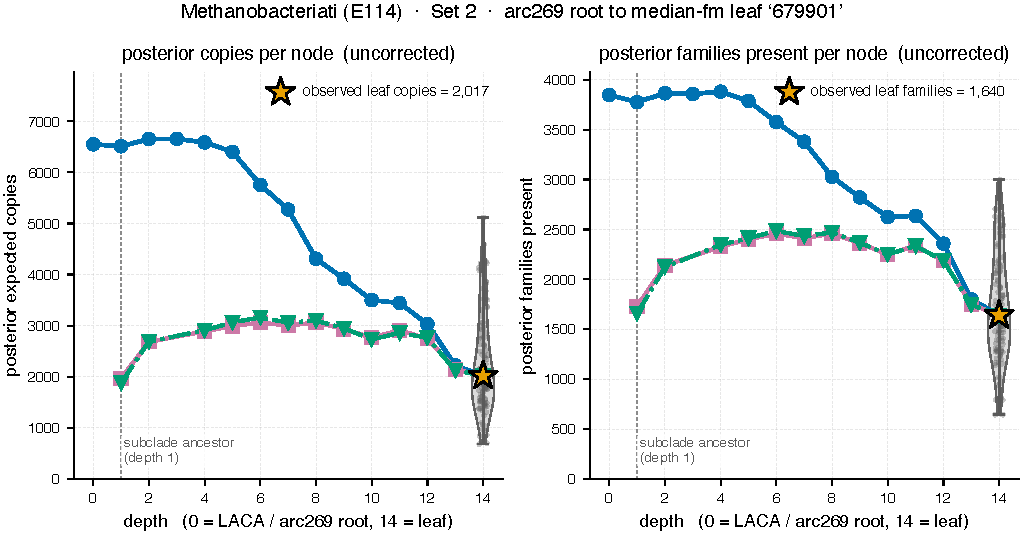
\includegraphics[width=0.92\linewidth,height=\textheight,keepaspectratio,alt={Methanobacteriati no-filter root-to-leaf path}]{../validation/outputs/min1_path_eury114.pdf}

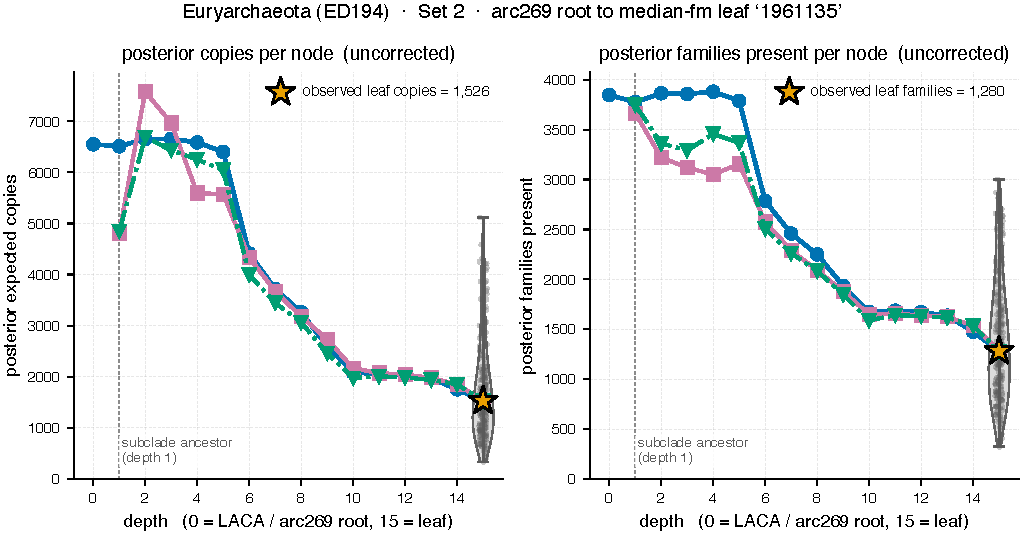
\includegraphics[width=0.92\linewidth,height=\textheight,keepaspectratio,alt={Euryarchaeota no-filter root-to-leaf path}]{../validation/outputs/min1_path_ed194.pdf}

\textbf{Figure 8.} No-filter (Set 2) root-to-leaf trajectories --- the
unfiltered arc269 fit and each subclade's own unfiltered fit, from the
arc269 root to the subclade's median-fm leaf.

\paragraph{Is the inflation a modelling
error?}\label{is-the-inflation-a-modelling-error}

No, and it is worth being precise about why not. Under any birth-death
process with a non-zero loss rate the ancestor is \emph{expected} to
hold more families than any one descendant: if a fraction p of the
ancestor's families survive to a given genome, that genome shows about p
· (ancestor size) families, so the ancestor exceeds it by about 1/p. An
ancestor richer than its descendants is the generic signature of
birth-death-with-loss, not a violation of the model.

The problem is not that GLD infers a large ancestor --- it is that GLD
on copy numbers \textbf{cannot apportion} that large ancestor between
the two histories it cannot tell apart: families genuinely present at
LACA and later lost, versus families that were never at LACA and reached
their modern spread by transfer. The inflated count is the honest output
of a correctly fitted model; it simply is not interpretable as an
ancestral genome size. The next section examines the filter Csurős uses
to bring the number down.

\subsubsection{3 --- The family-size filter, and why it does not rescue
the
inference}\label{3--the-family-size-filter-and-why-it-does-not-rescue-the-inference}

Csurős does not report the unfiltered ancestor. The published fits apply
a family-size filter --- keep only families with total copy count sum ≥
Ωmin, with Ωmin = 4 --- and the inferred ancestor that results is much
smaller. This section shows the filter has two problems: its threshold
is not derived from GLD, and applying it makes the fit to the
family-size data worse.

\paragraph{The filter shrinks the inferred
ancestor}\label{the-filter-shrinks-the-inferred-ancestor}

Apply each sum ≥ N filter (N ∈ \{1..10\}; N = 1 is no filter) to the
arc269 profile and refit. The inferred root shrinks monotonically as N
rises:

\textbf{Table 11.} arc269 filter sweep --- F, L(0) and inferred root
copies/families per sum ≥ N threshold.

\begin{center}
\begin{adjustbox}{max width=\textwidth}
\begin{tabular}{@{}lrrrrr@{}}
\toprule\noalign{}
arc269 fit & F & L(0) & root cp (raw / L(0)-amp) & root fm (raw /
L(0)-amp) & cp/fm \\
\midrule\noalign{}
no filter, mc=1 & 90,243 & 0.794 & 6,550 / 31,745 & 3,847 / 18,647 &
1.70 \\
sum ≥ 2 & 24,904 & 0.250 & 3,750 / 4,998 & 2,460 / 3,279 & 1.52 \\
sum ≥ 3 & 15,413 & 0.099 & 2,925 / 3,247 & 2,064 / 2,290 & 1.42 \\
\textbf{sum ≥ 4 (Csurös' threshold)} & 11,554 & 0.043 & 2,508 / 2,620 &
1,843 / 1,926 & \textbf{1.36} \\
sum ≥ 5 & 9,492 & 0.021 & 2,342 / 2,393 & 1,741 / 1,779 & 1.34 \\
sum ≥ 6 & 8,316 & 0.012 & 2,249 / 2,278 & 1,681 / 1,702 & 1.34 \\
sum ≥ 7 & 7,465 & 0.008 & 2,178 / 2,195 & 1,634 / 1,647 & 1.33 \\
sum ≥ 8 & 6,821 & 0.005 & 2,117 / 2,127 & 1,593 / 1,601 & 1.33 \\
sum ≥ 9 & 6,315 & 0.003 & 2,051 / 2,058 & 1,550 / 1,555 & 1.32 \\
sum ≥ 10 & 5,879 & 0.002 & 1,985 / 1,989 & 1,506 / 1,509 & 1.32 \\
\bottomrule\noalign{}
\end{tabular}
\end{adjustbox}
\end{center}

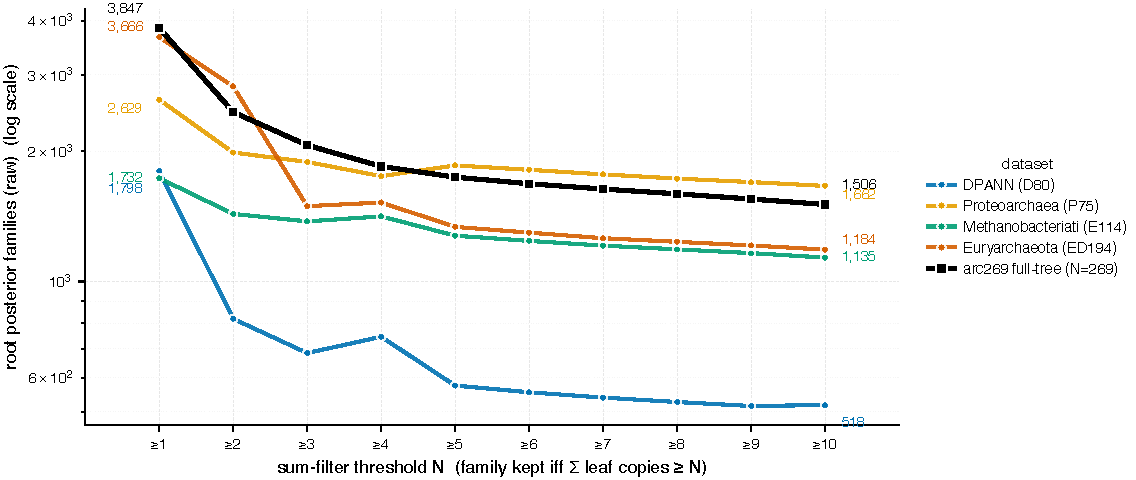
\includegraphics[width=0.92\linewidth,height=\textheight,keepaspectratio,alt={root families vs sum-filter threshold N, per dataset}]{../validation/outputs/sum_sweep_root_families.pdf}

\textbf{Figure 9.} Inferred root family count vs the sum ≥ N filter
threshold, for arc269 and each focal dataset. Generated by
\texttt{validation/sum\_sweep\_root\_summary.py}.

The root family count falls smoothly from 3,847 (no filter) to 1,506
(sum ≥ 10) --- and the same decline holds for the four focal subclades
fitted on their own genomes (Figure 9; the companion copy-count plot is
\texttt{validation/outputs/sum\_sweep\_root\_copies.png}). At Csurős'
Ωmin = 4 the root is 1,843 families --- less than half the unfiltered
estimate, and now within the range of modern genome sizes. The filter
does shrink the ancestor. The question is whether it shrinks it for a
principled reason.

\paragraph{The sweep traced along the root-to-leaf
path}\label{the-sweep-traced-along-the-root-to-leaf-path}

The shrinkage is not confined to the root node. Tracing each fit's
posterior count along the path from the deepest node down to a
subclade's median-fm leaf shows the whole ancestral half of the tree
moving with the threshold. Two plot sets follow. \textbf{Set 1.5} sweeps
the \emph{single} arc269 full-tree fit across sum ≥ 1..10 --- one GLD
fit to all 269 genomes at each threshold, its posterior then read along
each subclade's path. \textbf{Set 1} runs the same sum ≥ 1..10 sweep
\emph{per subclade}: each clade fitted on its own genomes alone, with no
information from the rest of the tree. The two sets use the same colour
and marker for the same threshold, so they can be read against each
other; sum ≥ 4, Csurős' canonical filter, is drawn bold with a
black-edged marker. The Set 1 subset fits are recount's reproductions of
Csurős' per-clade analysis --- run on the same family profiles they
recover his published per-clade fits (see
\hyperref[the-fits-analysed-here-are-csurux151s-fits]{The fits analysed
here are Csurős' fits} below).

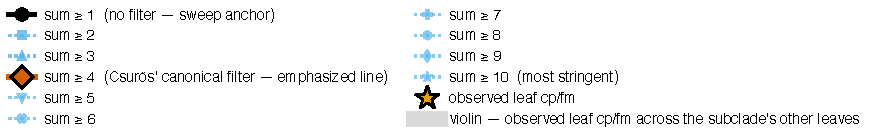
\includegraphics[width=0.92\linewidth,height=\textheight,keepaspectratio,alt={arc269 sum-filter sweep --- legend}]{../validation/outputs/arc269_sumsweep_path_legend.pdf}

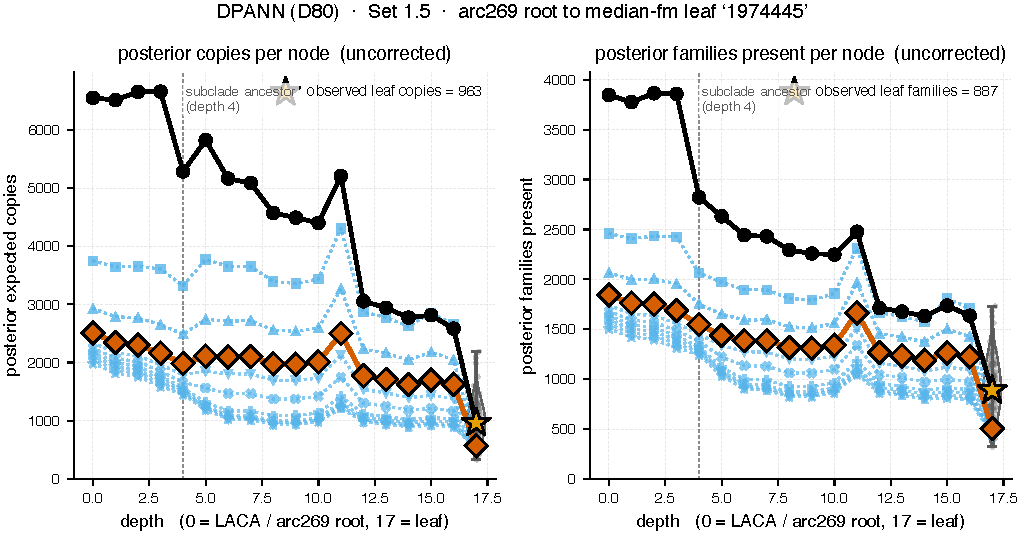
\includegraphics[width=0.92\linewidth,height=\textheight,keepaspectratio,alt={arc269 sum-sweep path, DPANN}]{../validation/outputs/arc269_sumsweep_path_dpann80.pdf}

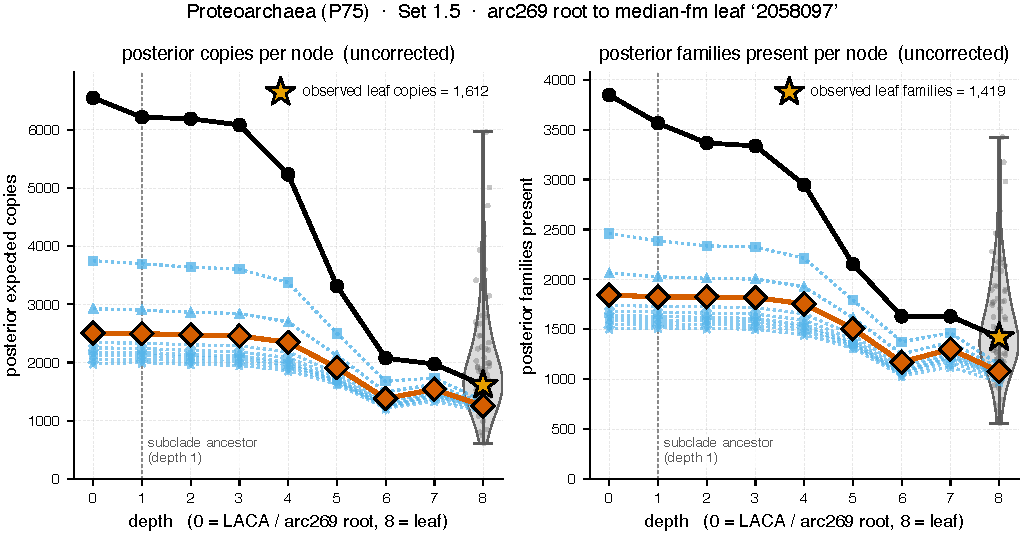
\includegraphics[width=0.92\linewidth,height=\textheight,keepaspectratio,alt={arc269 sum-sweep path, Proteoarchaea}]{../validation/outputs/arc269_sumsweep_path_proteo75.pdf}

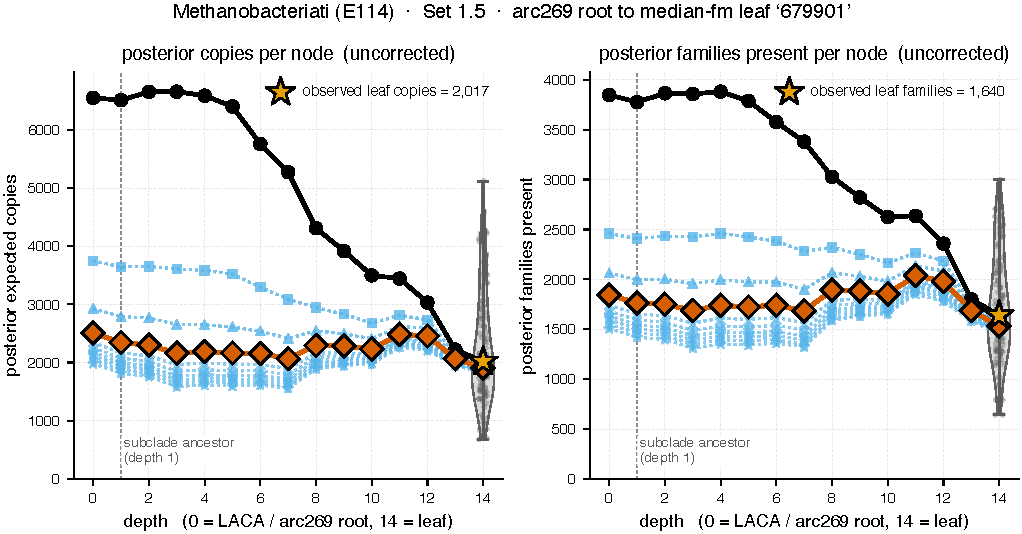
\includegraphics[width=0.92\linewidth,height=\textheight,keepaspectratio,alt={arc269 sum-sweep path, Methanobacteriati}]{../validation/outputs/arc269_sumsweep_path_eury114.pdf}

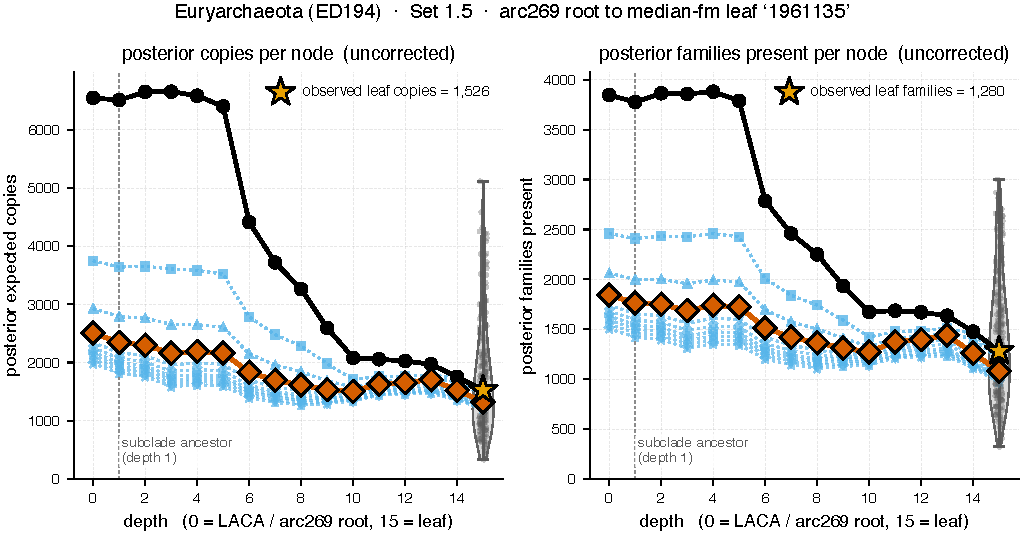
\includegraphics[width=0.92\linewidth,height=\textheight,keepaspectratio,alt={arc269 sum-sweep path, Euryarchaeota}]{../validation/outputs/arc269_sumsweep_path_ed194.pdf}

\textbf{Figure 10.} Set 1.5 --- the single arc269 full-tree fit swept
across sum ≥ 1..10, its posterior traced along each subclade's
root-to-leaf path.

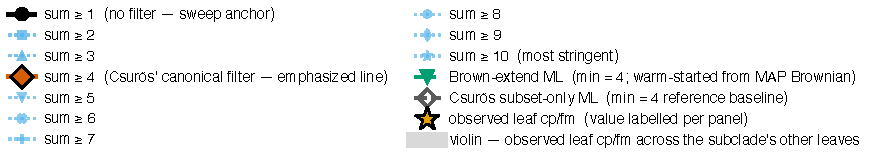
\includegraphics[width=0.92\linewidth,height=\textheight,keepaspectratio,alt={per-subclade sum-filter sweep --- legend}]{../validation/outputs/subset_min4_path_legend.pdf}

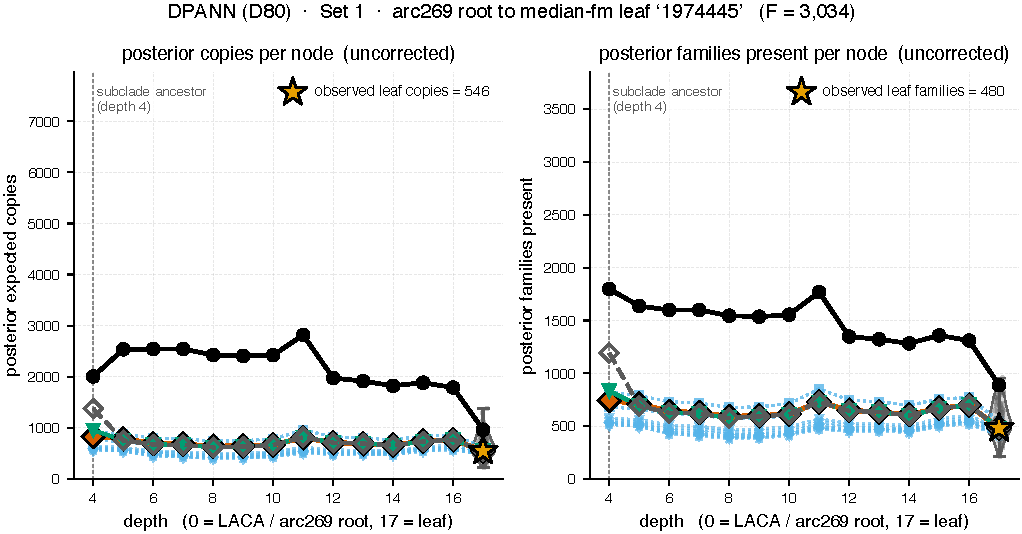
\includegraphics[width=0.92\linewidth,height=\textheight,keepaspectratio,alt={per-subclade sum-sweep path, DPANN}]{../validation/outputs/subset_min4_path_dpann80.pdf}

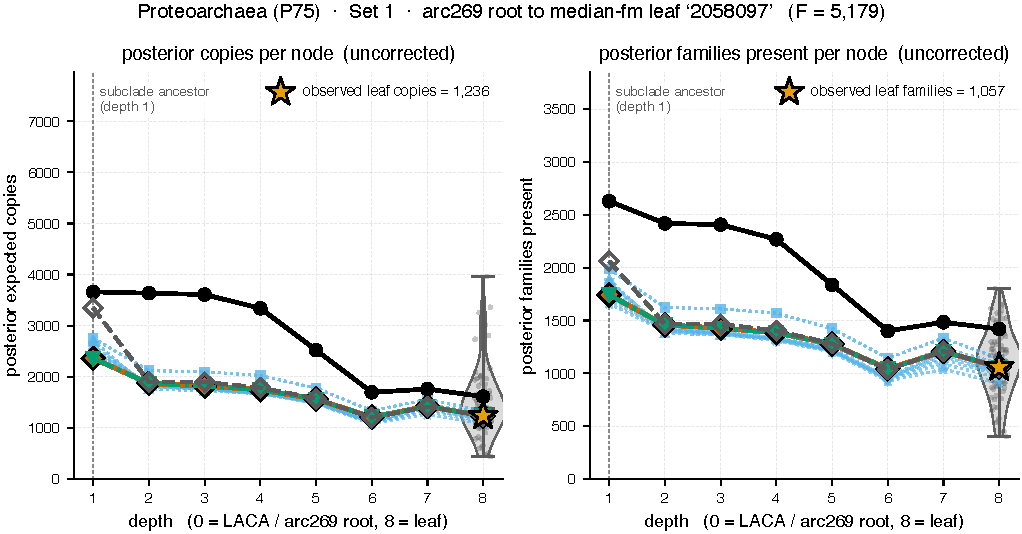
\includegraphics[width=0.92\linewidth,height=\textheight,keepaspectratio,alt={per-subclade sum-sweep path, Proteoarchaea}]{../validation/outputs/subset_min4_path_proteo75.pdf}

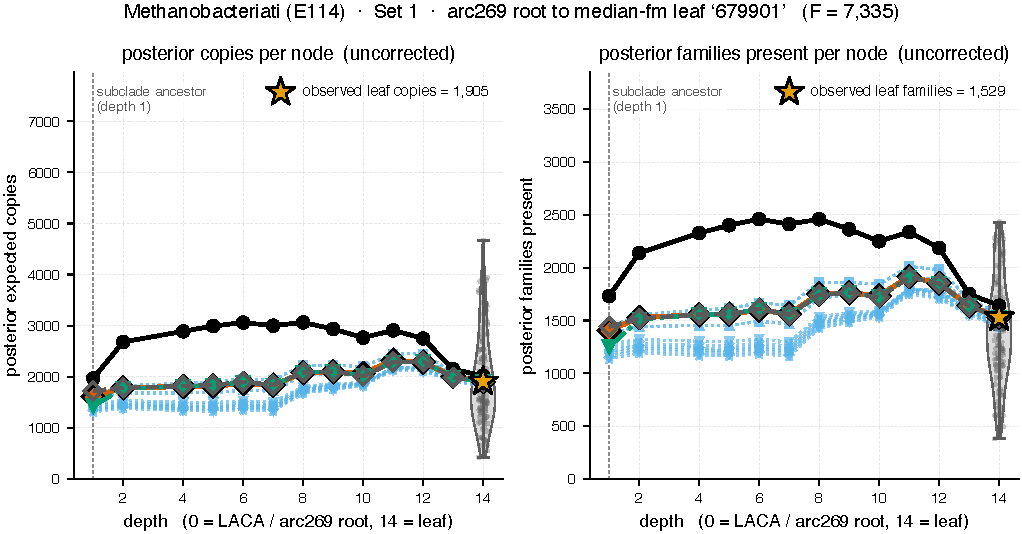
\includegraphics[width=0.92\linewidth,height=\textheight,keepaspectratio,alt={per-subclade sum-sweep path, Methanobacteriati}]{../validation/outputs/subset_min4_path_eury114.pdf}

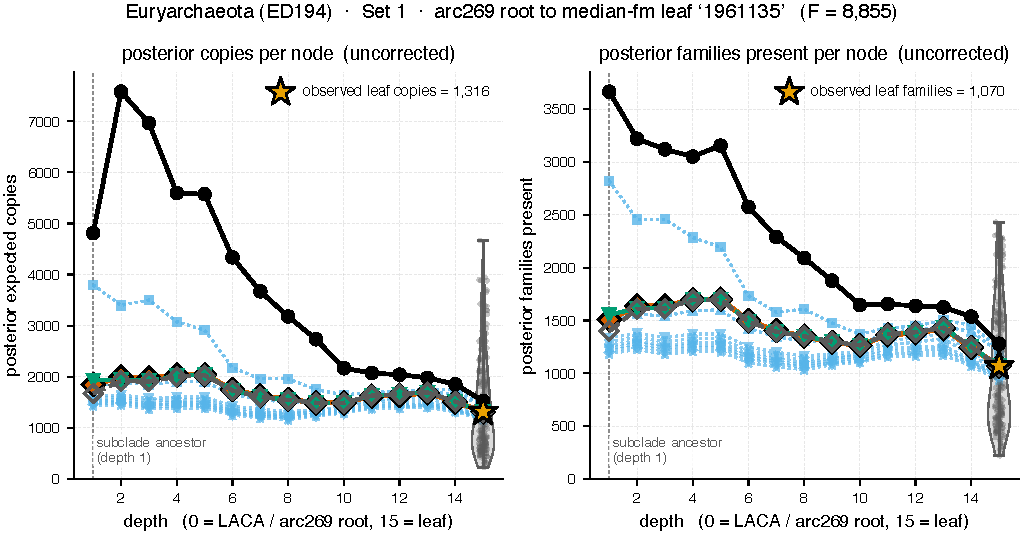
\includegraphics[width=0.92\linewidth,height=\textheight,keepaspectratio,alt={per-subclade sum-sweep path, Euryarchaeota}]{../validation/outputs/subset_min4_path_ed194.pdf}

\textbf{Figure 11.} Set 1 --- the same sum ≥ 1..10 sweep run per
subclade, each clade fitted on its own genomes, traced along its
root-to-leaf path.

Three things, read straight off Figures 10 and 11 and Table 11:

\begin{itemize}
\tightlist
\item
  \textbf{The threshold has a large effect.} From sum ≥ 1 to sum ≥ 10
  the inferred root family count changes by 1.5× to 3.5×, depending on
  the dataset: arc269 3,847 → 1,506 (factor 2.6); DPANN 1,798 → 518 and
  Euryarchaeota 3,666 → 1,184 (both ≈ 3×); Proteoarchaea 2,629 → 1,662
  and Methanobacteriati 1,732 → 1,135 (≈ 1.5×). The choice of threshold
  sets the answer to within a factor of two to three.
\item
  \textbf{Removing the singletons is not enough.} The single largest
  step in the sweep is sum ≥ 1 → sum ≥ 2 --- discarding the singletons
  --- but it does not settle the estimate: every later threshold moves
  it again. The arc269 sweep is monotone and still descending at sum ≥
  10 (≈ 3 \% per step, no plateau); after the singletons are gone the
  arc269 root still falls a further 39 \% (2,460 → 1,506). There is no N
  at which the inferred ancestor stops moving within the range tested.
\item
  \textbf{The effect is clade-dependent.} The four subclades do not
  shrink by the same factor --- DPANN and Euryarchaeota lose ≈ 3× of
  their root content across the sweep, Proteoarchaea and
  Methanobacteriati ≈ 1.5× --- so a threshold that discards one fraction
  of the small-family stratum in one clade discards a different fraction
  in another. (The per-subclade curves dip then rise slightly at N = 4:
  that point alone is read from Csurős' canonical min = 4 fit, run under
  the Ωmin = 4 observation-bias setting rather than the mc = 1 +
  pre-filter used at the other thresholds; the endpoints, and the arc269
  sweep, are unaffected.)
\end{itemize}

A further pattern emerges when the two sweeps are read against each
other at the \textbf{subclade ancestor} --- the deepest node at which
both a full-tree fit (Set 1.5) and a subset-only fit (Set 1) report a
value. The full-tree fit's response to the threshold is large and
roughly uniform across the four clades; the subset-only fits respond far
more unevenly. Each cell below gives the inferred family count at that
clade's ancestor at sum ≥ 1 (no filter) and at sum ≥ 10, with the sweep
ratio (uncorrected posterior counts):

\textbf{Table 12.} Inferred family count at each subclade ancestor at
sum ≥ 1 vs sum ≥ 10, full-tree fit vs subset-only fit.

\begin{center}
\begin{adjustbox}{max width=\textwidth}
\begin{tabular}{@{}lrr@{}}
\toprule\noalign{}
subclade ancestor & full-tree fit (Set 1.5) & subset-only fit (Set 1) \\
\midrule\noalign{}
DPANN & 2,822 → 1,245 (× 2.3) & 1,798 → 518 (× 3.5) \\
Proteoarchaea & 3,565 → 1,515 (× 2.4) & 2,629 → 1,662 (× 1.6) \\
Methanobacteriati & 3,777 → 1,421 (× 2.7) & 1,732 → 1,135 (× 1.5) \\
Euryarchaeota & 3,777 → 1,421 (× 2.7) & 3,666 → 1,184 (× 3.1) \\
\bottomrule\noalign{}
\end{tabular}
\end{adjustbox}
\end{center}

Methanobacteriati and Euryarchaeota resolve to the same ancestral node
in the arc269 tree, so the full-tree fit reports one value for both.
Across the sweep the full-tree fit moves its estimate of every clade
ancestor by × 2.3--2.7 on families (× 3.1--3.6 on copies). The
subset-only fits split in two: the DPANN and Euryarchaeota ancestors
move ≈ 3× --- as much as the full-tree fit --- but the Proteoarchaea and
Methanobacteriati ancestors move only ≈ 1.5×. For those two clades the
family-size filter is a much heavier knob in the full-tree fit than in
the clade-alone fit: the threshold change that barely shifts the
Proteoarchaea or Methanobacteriati ancestor when the clade is fitted on
its own moves the full-tree fit's estimate of the \emph{same node} by
1.5--1.7× as much (2.0--2.4× on copies). The threshold's influence on
the inferred ancestor is contingent twice over --- on the clade, and on
whether that clade was fitted alone or as part of the whole tree.

The data do not single out a threshold: the estimate is a continuous,
unplateaued function of N, and the per-clade effect differs, so no one N
is simultaneously the natural cut for all four clades. Csurős' reasons
for N = 4 (next subsection) come from outside this sweep.

\paragraph{Problem 1 --- the threshold Ωmin = 4 is not a property of
GLD}\label{problem-1--the-threshold-ux3c9min--4-is-not-a-property-of-gld}

Why four? Csurős 2026 PNAS (p. 2) gives the reason: comparability with
gene-tree reconciliation methods, which need at least four copies of a
family before its unrooted gene tree carries any topological signal.
That is a genuine rationale --- but it is a property of
\emph{reconciliation}, not of GLD. The GLD likelihood places no lower
bound on family size; it is defined for a family of any size, and the
Ωmin sampling-bias correction is defined for any Ωmin ≥ 1, including
Ωmin = 1 (no filter). Nothing inside GLD selects four, or selects any
threshold at all.

And the inferred ancestor depends strongly on the choice. The sweep in
Table 11 is smooth and monotone --- root family count 3,847 → 2,460 →
2,064 → 1,843 → \ldots{} → 1,506 as N runs 1 → 10 --- with no elbow, no
plateau, no value the data singles out. Csurős' own SI reports fits at
Ωmin = 4, 2 and 1 and notes that the inferred history shifts with the
threshold. The ancestral genome size GLD reports is therefore set, to
better than a factor of two, by a knob whose value is imported from the
requirements of a different method.

\paragraph{Problem 2 --- filtering makes the fit to the family-size data
worse}\label{problem-2--filtering-makes-the-fit-to-the-family-size-data-worse}

Return to the goodness-of-fit tables (Tables 7--9) in section 2. The
unfiltered \texttt{mc\ =\ 1} fit reproduces the empirical family-size
histogram (ratios 0.94--1.29). Every filtered fit fails it, and fails it
worse the stronger the filter:

\begin{itemize}
\tightlist
\item
  at Csurős' Ωmin = 4 the predicted/empirical ratios run from 0.01 at k
  = 1 to 1.35 at k ≥ 8 --- the filtered rate process predicts far too
  few small families and too many large ones;
\item
  the conditional tests rule out ``it is only the singletons'':
  re-normalised to drop singletons (Ω ≥ 2) the sum ≥ 4 ratios still span
  0.17--2.56, and dropping 1- and 2-copy families (Ω ≥ 3) they span
  0.24--1.70. The \emph{shape} of the predicted distribution is wrong on
  the families the filter keeps, not only on the families it discards;
\item
  the misfit grows monotonically with the threshold: at sum ≥ 10 the Ω ≥
  2 ratios span 0.03--3.27.
\end{itemize}

So filtering does not solve the problem; it moves it. The unfiltered fit
reproduces the family-size data, but its ancestor is inflated past any
living genome and --- by section 1 --- transfer- confounded. The
filtered fit returns a smaller, modern-sized ancestor, but it no longer
reproduces the family-size data, the threshold that set its size is
arbitrary, and the ancestor is still transfer-confounded: dropping the
small families lowers the count but does not give the likelihood the
gene-tree signal it would need to separate inheritance from transfer. No
filter setting yields an ancestral estimate that is at once consistent
with the family-size data and free of the transfer ambiguity --- the
second is not something a copy-number filter can buy.

\paragraph{The fits analysed here are Csurős'
fits}\label{the-fits-analysed-here-are-csurux151s-fits}

The critique above is of the published analysis, not of a re-fit that
happens to behave differently. Evaluated at the four subclade ancestors,
the recount fit on the union of the per-subclade sum ≥ 4 family sets
matches Csurős' published per-clade fits to within 0.88--1.28 on
ancestral family count:

\textbf{Table 13.} Ancestral family count at each subclade ancestor ---
Csurős' published per-clade sum ≥ 4 fit vs the recount union-sum ≥ 4
fit.

\begin{center}
\begin{adjustbox}{max width=\textwidth}
\begin{tabular}{@{}lrrr@{}}
\toprule\noalign{}
subclade ancestor & Csurős per-clade sum ≥ 4 fm & recount union-sum ≥ 4
fm & ratio \\
\midrule\noalign{}
DPANN & 1,210 & 1,553 & 1.28 \\
Proteoarchaea & 2,096 & 1,841 & 0.88 \\
Methanobacteriati & 1,453 & 1,772 & 1.22 \\
Euryarchaeota & 1,419 & 1,772 & 1.25 \\
\bottomrule\noalign{}
\end{tabular}
\end{adjustbox}
\end{center}

The per-branch rates agree to within 10--30 \% on the gain axis for
three of the four subclades (median ratio 0.71--1.11; DPANN is the
exception --- long-branch artefacts are a plausible cause) and to within
25 \% on branch length. The
\hyperref[demonstration-of-reproduction]{reproduction tables} (Tables
2--5) make the same point on log-likelihood: recount's recommended fits
land within a few nat of Csurős' published rates on every dataset. The
behaviour analysed here is the behaviour of the published GLD analysis.

The Set 3 path plots (Figure 12) show this agreement node by node. Each
panel traces the single arc269 full-tree fit on the union-sum ≥ 4
universe (seagreen) alongside Csurős' published per-clade subset-only ML
(gray) and recount's two per-clade fits (MAP Brownian, Brownian-extend
ML), from the arc269 root to a subclade's median-fm leaf. Over the
stretch where both a full-tree and a per-clade fit are defined --- from
the subclade ancestor leafward --- the seagreen and gray lines run close
together: the node-by-node form of the 0.88--1.28 ancestral agreement of
Table 13.

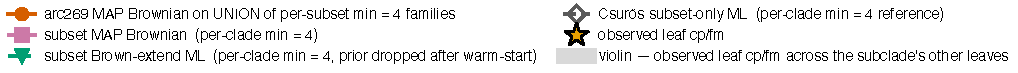
\includegraphics[width=0.92\linewidth,height=\textheight,keepaspectratio,alt={Set 3 --- union-min4 full-tree fit vs Csurős per-clade reference, legend}]{../validation/outputs/union_path_legend.pdf}

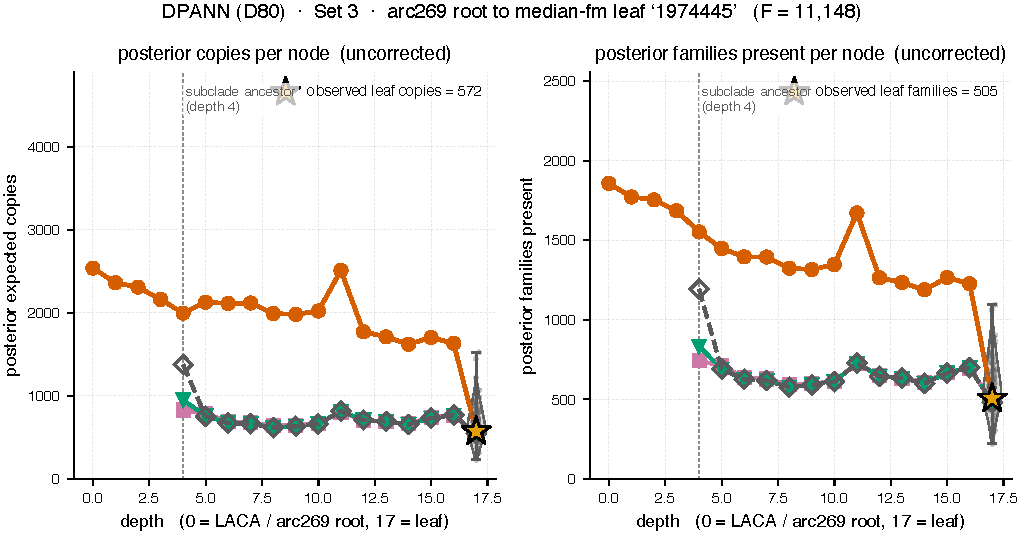
\includegraphics[width=0.92\linewidth,height=\textheight,keepaspectratio,alt={Set 3 union-min4 path, DPANN}]{../validation/outputs/union_path_dpann80.pdf}

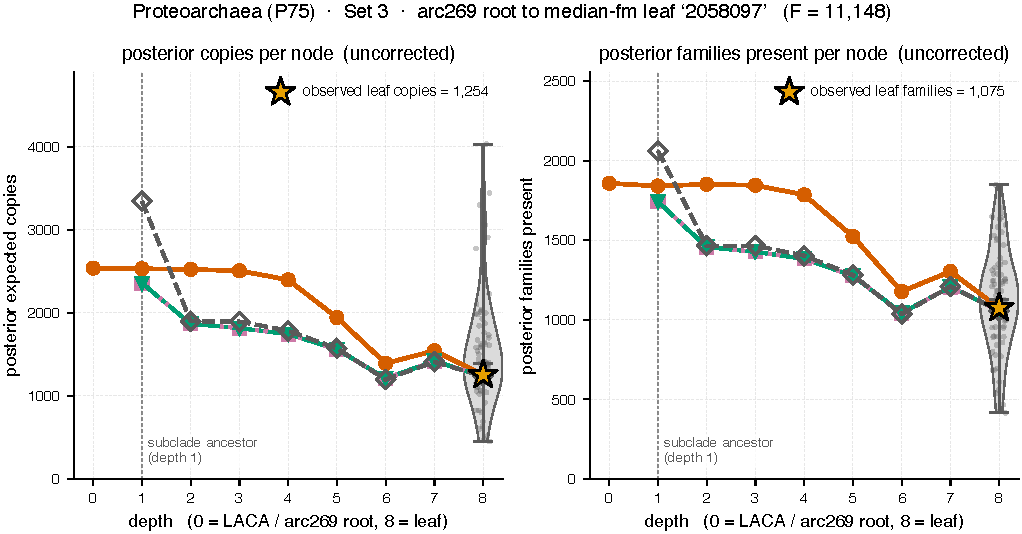
\includegraphics[width=0.92\linewidth,height=\textheight,keepaspectratio,alt={Set 3 union-min4 path, Proteoarchaea}]{../validation/outputs/union_path_proteo75.pdf}

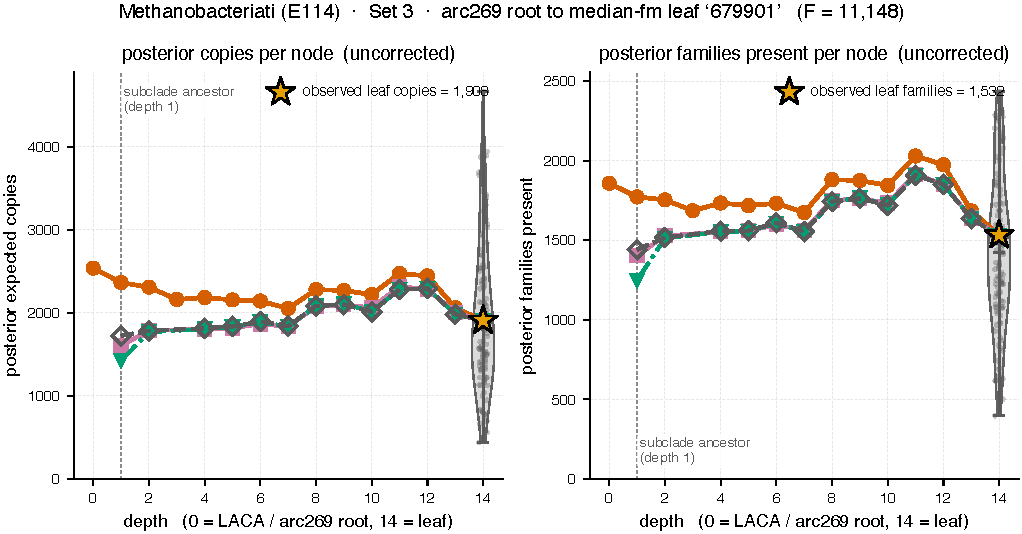
\includegraphics[width=0.92\linewidth,height=\textheight,keepaspectratio,alt={Set 3 union-min4 path, Methanobacteriati}]{../validation/outputs/union_path_eury114.pdf}

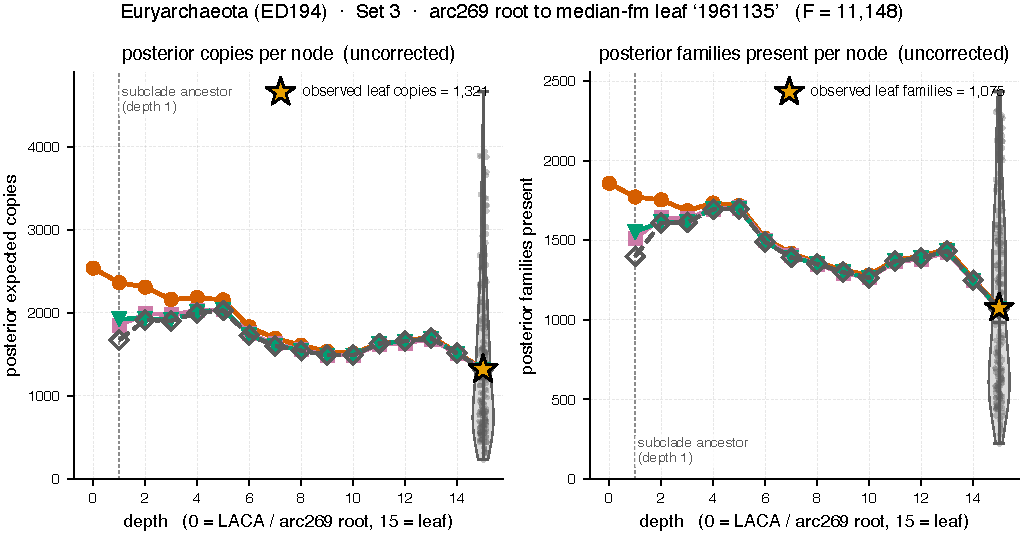
\includegraphics[width=0.92\linewidth,height=\textheight,keepaspectratio,alt={Set 3 union-min4 path, Euryarchaeota}]{../validation/outputs/union_path_ed194.pdf}

\textbf{Figure 12.} Set 3 --- the arc269 full-tree fit on the union-sum
≥ 4 universe traced against Csurős' per-clade reference and recount's
two per-clade fits, root to median-fm leaf.

The L(0)-amplified counterparts are in
\hyperref[l0-corrected-trajectories]{L(0)-corrected trajectories} at the
end of this README.

\paragraph{Characterising the filtered ancestor: the LACA
CORE}\label{characterising-the-filtered-ancestor-the-laca-core}

Take the filtered fit at face value for a moment. From the per-family
posteriors of the arc269 fit on the union of the per-subclade sum ≥ 4
families (F = 11,148 --- the fit that reproduces Csurős' published
per-clade numbers, above), define the inferred ancestral core as the
families the model places at the root with posterior probability at
least one-half:

LACA CORE = \{ families with P(present at the arc269 root) ≥ 0.5 \}

--- 1,817 families. The natural check on a putative ancestral core is
how it is distributed across the modern genomes that descend from it:

\textbf{Table 14.} Distribution of the 1,817-family LACA CORE across
each subclade's modern genomes.

\begin{center}
\begin{adjustbox}{max width=\textwidth}
\begin{tabular}{@{}lrrr@{}}
\toprule\noalign{}
subclade & LACA-CORE families in ≥ 90 \% of the subclade's genomes &
\ldots in every genome & median per-genome retention \\
\midrule\noalign{}
DPANN & 1.7 \% & 1 family & 20 \% \\
Proteoarchaea & 4.1 \% & 1 family & 45 \% \\
Methanobacteriati & 13.5 \% & 1 family & 52 \% \\
Euryarchaeota & 3.2 \% & 0 families & 41 \% \\
\bottomrule\noalign{}
\end{tabular}
\end{adjustbox}
\end{center}

Not one of the 1,817 inferred-ancestral families is present in every
genome of even a single subclade, and the median modern genome carries
only 20--52 \% of the inferred core. That is a strikingly patchy object
for a putative ancestral genome. But patchiness is consistent with two
readings --- heavy lineage-specific \emph{loss} of a genuinely ancestral
core, or a core that is partly \emph{transfer-spread} families that were
never ancestral --- and, by section 1, copy numbers cannot tell the two
apart. The characterization is reported for completeness; it does not,
on its own, decide the question. Full per-threshold tables are in the
\hyperref[supporting-data]{supporting tables} below; the figure and
tables are regenerated by \texttt{validation/laca\_core\_analysis.py}.

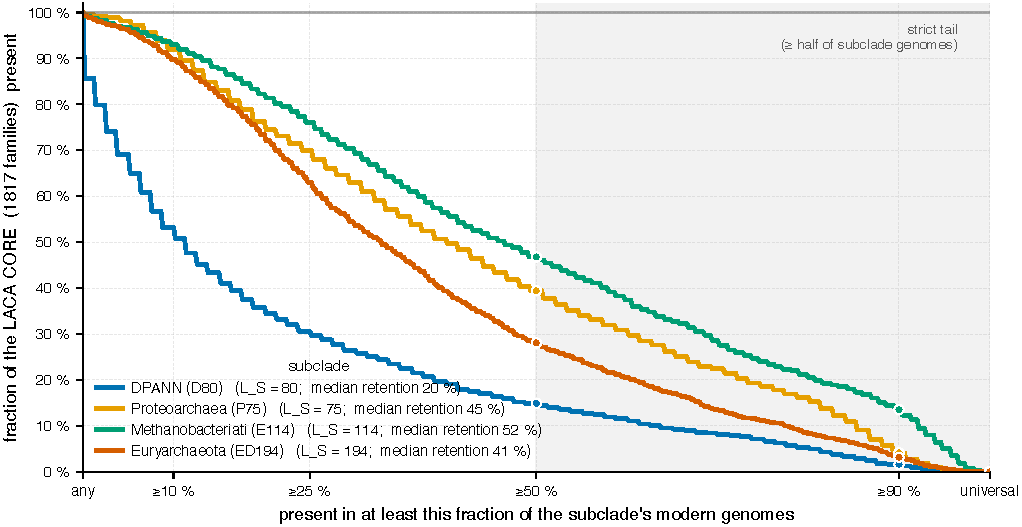
\includegraphics[width=0.92\linewidth,height=\textheight,keepaspectratio,alt={LACA CORE distribution across subclade genomes}]{../validation/outputs/laca_core_subset_distribution.pdf}

\textbf{Figure 13.} Distribution of the LACA CORE families across the
genomes of each subclade.

\subsubsection{4 --- Conclusion}\label{4--conclusion}

The \hyperref[demonstration-of-reproduction]{reproduction section}
confirms that the GLD likelihood, its gradient and the Ωmin
sampling-bias correction are correctly implemented, and that recount's
fits recover Csurős' published rates to within a few nat. As a
likelihood of gene-copy-number data, the GLD model is exactly what the
paper says it is.

The claim tested in this section is the narrower one in the abstract's
closing sentence --- that the framework is \emph{``a statistically sound
foundation for hypothesizing about gene content evolution across the
diversity of entire kingdoms.''} On the arc269 archaeal data it is not,
for three reasons that compound:

\begin{itemize}
\tightlist
\item
  \textbf{Copy numbers do not identify ancestry when transfer is
  present.} A transferred family and a genuinely inherited one can carry
  the same copy-number profile, and GLD --- whose model has no transfer
  edge --- gives the two the same ancestral posterior; it cannot tell
  them apart (section 1). Because a transferred family's true ancestral
  contribution is zero, every cross-clade transfer biases the inferred
  ancestor upward. Archaea are a transfer-rich kingdom, so this is the
  typical case, not an edge case.
\item
  \textbf{Unfiltered, GLD fits the family-size data and infers an
  ancestor larger than any living archaeon.} The no-filter fit
  reproduces the empirical family-size distribution to within 10--30 \%
  per bin, yet places 3,847 families at LACA --- above the richest
  modern archaeal genome --- and its own extinction correction raises
  that to ≈ 18,600 (section 2). The inflation is not an optimisation
  failure --- the fit is faithful to the family-size data --- and copy
  numbers cannot say what share of the inferred ancestor is genuine
  ancestral content and what share is transfer-spread families read as
  ancestral.
\item
  \textbf{The filter that suppresses the inflation is unprincipled and
  degrades the fit.} Ωmin = 4 is imported from the requirements of
  gene-tree reconciliation, not from GLD; the inferred ancestor is a
  smooth function of the threshold with no value the data selects; and
  every filtered fit describes the family-size distribution worse than
  the unfiltered fit, whether or not the singleton stratum is excluded
  (section 3).
\end{itemize}

No setting of the copy-number-only GLD framework delivers, at the same
time, a rate process consistent with the observed family-size
distribution and an ancestral genome estimate not confounded by
transfer. Unfiltered, the fit is faithful to the data and the ancestor
is not credible. Filtered, the ancestor is modern-sized but the fit is
no longer faithful to the data, the threshold is arbitrary, and ---
because the family-size filter does not change what the likelihood can
see --- the identifiability gap of section 1 remains: the smaller
ancestor is still a mixture of inherited and transfer-spread families
that copy numbers cannot separate.

This is a limitation of the \emph{input}, not of the algorithm. Gene
copy numbers alone do not carry the signal that separates vertical
inheritance from horizontal transfer; the within-family signal that does
--- gene-tree topology, sampled from sequence alignments --- is what
reconciliation methods consume and GLD does not. A copy-number
likelihood, however correctly implemented, is therefore not a sufficient
foundation for ancestral gene-content inference in a kingdom shaped by
transfer. That is the specific sense in which the analysis here does not
support the closing claim of Csurős 2026.

\subsection{Supporting data}\label{supporting-data}

\subsubsection{Filter-sensitivity tables: per-leaf retention of M\_N
across thresholds N =
1..10}\label{filter-sensitivity-tables-per-leaf-retention-of-m_n-across-thresholds-n--110}

A model-free companion to the LACA CORE characterization above. For
subset S with leaves L\_S, threshold N, and filter family universe M\_N
= \{ f : Σ over v ∈ L\_S of profile{[}f, v{]} ≥ N \}, define

r\_v(N) = \textbar\{ f ∈ M\_N : profile{[}f, v{]} ≥ 1 \}\textbar{} /
\textbar M\_N\textbar{}

--- the fraction of the filter family universe present at extant genome
v. The tables below (Tables 15--24) report this distribution per
threshold N alongside the model's posterior fm at the subset root
(Csurös subset-only ML at N = 4; per-subset Brownian MAP at the other N)
and the ``universal'' / ``≥ 90 \% of leaves'' counts.

\subparagraph{N = 1 (no filter applied)}\label{n--1-no-filter-applied}

\textbf{Table 15.} Per-leaf retention of the filter family universe M\_N
at threshold N = 1 (no filter), per subset.

\begin{center}
\begin{adjustbox}{max width=\textwidth}
\begin{tabular}{@{}lrrrrrrrrrrr@{}}
\toprule\noalign{}
subset & L\_S & F\_N & root\_fm & r\_p10 & r\_p50 & r\_p90 & r\_max &
universal & ≥90 \% lvs & \%univ & \%≥90 \% \\
\midrule\noalign{}
DPANN & 80 & 28,576 & 1,798 & 0.020 & 0.031 & 0.045 & 0.061 & 1 & 30 &
0.00 & 0.10 \\
Proteo & 75 & 33,547 & 2,629 & 0.031 & 0.042 & 0.065 & 0.102 & 1 & 75 &
0.00 & 0.22 \\
Methano & 114 & 37,609 & 1,732 & 0.031 & 0.044 & 0.067 & 0.080 & 1 & 246
& 0.00 & 0.65 \\
Eury & 194 & 62,435 & 3,666 & 0.012 & 0.021 & 0.038 & 0.048 & 0 & 58 &
0.00 & 0.09 \\
\bottomrule\noalign{}
\end{tabular}
\end{adjustbox}
\end{center}

\subparagraph{N = 2}\label{n--2}

\textbf{Table 16.} Per-leaf retention of M\_N at threshold N = 2, per
subset.

\begin{center}
\begin{adjustbox}{max width=\textwidth}
\begin{tabular}{@{}lrrrrrrrrrrr@{}}
\toprule\noalign{}
subset & L\_S & F\_N & root\_fm & r\_p10 & r\_p50 & r\_p90 & r\_max &
universal & ≥90 \% lvs & \%univ & \%≥90 \% \\
\midrule\noalign{}
DPANN & 80 & 6,632 & 820 & 0.067 & 0.096 & 0.135 & 0.178 & 1 & 30 & 0.02
& 0.45 \\
Proteo & 75 & 10,746 & 1,985 & 0.073 & 0.111 & 0.160 & 0.213 & 1 & 75 &
0.01 & 0.70 \\
Methano & 114 & 13,257 & 1,432 & 0.067 & 0.114 & 0.168 & 0.195 & 1 & 246
& 0.01 & 1.86 \\
Eury & 194 & 17,637 & 2,821 & 0.030 & 0.062 & 0.111 & 0.147 & 0 & 58 &
0.00 & 0.33 \\
\bottomrule\noalign{}
\end{tabular}
\end{adjustbox}
\end{center}

\subparagraph{N = 3}\label{n--3}

\textbf{Table 17.} Per-leaf retention of M\_N at threshold N = 3, per
subset.

\begin{center}
\begin{adjustbox}{max width=\textwidth}
\begin{tabular}{@{}lrrrrrrrrrrr@{}}
\toprule\noalign{}
subset & L\_S & F\_N & root\_fm & r\_p10 & r\_p50 & r\_p90 & r\_max &
universal & ≥90 \% lvs & \%univ & \%≥90 \% \\
\midrule\noalign{}
DPANN & 80 & 4,084 & 683 & 0.101 & 0.144 & 0.201 & 0.253 & 1 & 30 & 0.02
& 0.73 \\
Proteo & 75 & 6,694 & 1,888 & 0.105 & 0.169 & 0.241 & 0.305 & 1 & 75 &
0.01 & 1.12 \\
Methano & 114 & 9,202 & 1,376 & 0.092 & 0.156 & 0.236 & 0.271 & 1 & 246
& 0.01 & 2.67 \\
Eury & 194 & 11,515 & 1,492 & 0.042 & 0.088 & 0.165 & 0.217 & 0 & 58 &
0.00 & 0.50 \\
\bottomrule\noalign{}
\end{tabular}
\end{adjustbox}
\end{center}

\subparagraph{N = 4 (Csurös' canonical
threshold)}\label{n--4-csuruxf6s-canonical-threshold}

\textbf{Table 18.} Per-leaf retention of M\_N at the canonical threshold
N = 4, per subset.

\begin{center}
\begin{adjustbox}{max width=\textwidth}
\begin{tabular}{@{}lrrrrrrrrrrr@{}}
\toprule\noalign{}
subset & L\_S & F\_N & root\_fm & r\_p10 & r\_p50 & r\_p90 & r\_max &
universal & ≥90 \% lvs & \%univ & \%≥90 \% \\
\midrule\noalign{}
DPANN & 80 & 3,034 & 1,192 & 0.124 & 0.180 & 0.255 & 0.315 & 1 & 30 &
0.03 & 0.99 \\
Proteo & 75 & 5,179 & 2,062 & 0.131 & 0.214 & 0.294 & 0.348 & 1 & 75 &
0.02 & 1.45 \\
Methano & 114 & 7,335 & 1,441 & 0.108 & 0.193 & 0.289 & 0.331 & 1 & 246
& 0.01 & 3.35 \\
Eury & 194 & 8,855 & 1,399 & 0.052 & 0.110 & 0.212 & 0.275 & 0 & 58 &
0.00 & 0.65 \\
\bottomrule\noalign{}
\end{tabular}
\end{adjustbox}
\end{center}

\subparagraph{N = 5}\label{n--5}

\textbf{Table 19.} Per-leaf retention of M\_N at threshold N = 5, per
subset.

\begin{center}
\begin{adjustbox}{max width=\textwidth}
\begin{tabular}{@{}lrrrrrrrrrrr@{}}
\toprule\noalign{}
subset & L\_S & F\_N & root\_fm & r\_p10 & r\_p50 & r\_p90 & r\_max &
universal & ≥90 \% lvs & \%univ & \%≥90 \% \\
\midrule\noalign{}
DPANN & 80 & 2,481 & 575 & 0.148 & 0.212 & 0.296 & 0.363 & 1 & 30 & 0.04
& 1.21 \\
Proteo & 75 & 4,285 & 1,853 & 0.150 & 0.254 & 0.338 & 0.378 & 1 & 75 &
0.02 & 1.75 \\
Methano & 114 & 6,308 & 1,276 & 0.114 & 0.219 & 0.331 & 0.375 & 1 & 246
& 0.02 & 3.90 \\
Eury & 194 & 7,454 & 1,337 & 0.060 & 0.129 & 0.247 & 0.318 & 0 & 58 &
0.00 & 0.78 \\
\bottomrule\noalign{}
\end{tabular}
\end{adjustbox}
\end{center}

\subparagraph{N = 6}\label{n--6}

\textbf{Table 20.} Per-leaf retention of M\_N at threshold N = 6, per
subset.

\begin{center}
\begin{adjustbox}{max width=\textwidth}
\begin{tabular}{@{}lrrrrrrrrrrr@{}}
\toprule\noalign{}
subset & L\_S & F\_N & root\_fm & r\_p10 & r\_p50 & r\_p90 & r\_max &
universal & ≥90 \% lvs & \%univ & \%≥90 \% \\
\midrule\noalign{}
DPANN & 80 & 2,166 & 555 & 0.164 & 0.236 & 0.324 & 0.393 & 1 & 30 & 0.05
& 1.39 \\
Proteo & 75 & 3,659 & 1,810 & 0.170 & 0.289 & 0.372 & 0.415 & 1 & 75 &
0.03 & 2.05 \\
Methano & 114 & 5,709 & 1,241 & 0.123 & 0.237 & 0.360 & 0.406 & 1 & 246
& 0.02 & 4.31 \\
Eury & 194 & 6,691 & 1,297 & 0.066 & 0.142 & 0.272 & 0.348 & 0 & 58 &
0.00 & 0.87 \\
\bottomrule\noalign{}
\end{tabular}
\end{adjustbox}
\end{center}

\subparagraph{N = 7}\label{n--7}

\textbf{Table 21.} Per-leaf retention of M\_N at threshold N = 7, per
subset.

\begin{center}
\begin{adjustbox}{max width=\textwidth}
\begin{tabular}{@{}lrrrrrrrrrrr@{}}
\toprule\noalign{}
subset & L\_S & F\_N & root\_fm & r\_p10 & r\_p50 & r\_p90 & r\_max &
universal & ≥90 \% lvs & \%univ & \%≥90 \% \\
\midrule\noalign{}
DPANN & 80 & 1,893 & 539 & 0.184 & 0.258 & 0.357 & 0.418 & 1 & 30 & 0.05
& 1.58 \\
Proteo & 75 & 3,268 & 1,767 & 0.185 & 0.318 & 0.407 & 0.442 & 1 & 75 &
0.03 & 2.29 \\
Methano & 114 & 5,268 & 1,210 & 0.129 & 0.255 & 0.384 & 0.433 & 1 & 246
& 0.02 & 4.67 \\
Eury & 194 & 6,089 & 1,258 & 0.071 & 0.155 & 0.295 & 0.375 & 0 & 58 &
0.00 & 0.95 \\
\bottomrule\noalign{}
\end{tabular}
\end{adjustbox}
\end{center}

\subparagraph{N = 8}\label{n--8}

\textbf{Table 22.} Per-leaf retention of M\_N at threshold N = 8, per
subset.

\begin{center}
\begin{adjustbox}{max width=\textwidth}
\begin{tabular}{@{}lrrrrrrrrrrr@{}}
\toprule\noalign{}
subset & L\_S & F\_N & root\_fm & r\_p10 & r\_p50 & r\_p90 & r\_max &
universal & ≥90 \% lvs & \%univ & \%≥90 \% \\
\midrule\noalign{}
DPANN & 80 & 1,718 & 527 & 0.198 & 0.274 & 0.378 & 0.435 & 1 & 30 & 0.06
& 1.75 \\
Proteo & 75 & 2,962 & 1,728 & 0.202 & 0.341 & 0.437 & 0.470 & 1 & 75 &
0.03 & 2.53 \\
Methano & 114 & 4,916 & 1,186 & 0.136 & 0.269 & 0.406 & 0.455 & 1 & 246
& 0.02 & 5.00 \\
Eury & 194 & 5,674 & 1,235 & 0.075 & 0.165 & 0.314 & 0.396 & 0 & 58 &
0.00 & 1.02 \\
\bottomrule\noalign{}
\end{tabular}
\end{adjustbox}
\end{center}

\subparagraph{N = 9}\label{n--9}

\textbf{Table 23.} Per-leaf retention of M\_N at threshold N = 9, per
subset.

\begin{center}
\begin{adjustbox}{max width=\textwidth}
\begin{tabular}{@{}lrrrrrrrrrrr@{}}
\toprule\noalign{}
subset & L\_S & F\_N & root\_fm & r\_p10 & r\_p50 & r\_p90 & r\_max &
universal & ≥90 \% lvs & \%univ & \%≥90 \% \\
\midrule\noalign{}
DPANN & 80 & 1,573 & 516 & 0.215 & 0.294 & 0.400 & 0.454 & 1 & 30 & 0.06
& 1.91 \\
Proteo & 75 & 2,727 & 1,696 & 0.217 & 0.367 & 0.462 & 0.498 & 1 & 75 &
0.04 & 2.75 \\
Methano & 114 & 4,610 & 1,163 & 0.143 & 0.283 & 0.425 & 0.474 & 1 & 246
& 0.02 & 5.34 \\
Eury & 194 & 5,296 & 1,211 & 0.079 & 0.175 & 0.333 & 0.414 & 0 & 58 &
0.00 & 1.10 \\
\bottomrule\noalign{}
\end{tabular}
\end{adjustbox}
\end{center}

\subparagraph{N = 10}\label{n--10}

\textbf{Table 24.} Per-leaf retention of M\_N at threshold N = 10, per
subset.

\begin{center}
\begin{adjustbox}{max width=\textwidth}
\begin{tabular}{@{}lrrrrrrrrrrr@{}}
\toprule\noalign{}
subset & L\_S & F\_N & root\_fm & r\_p10 & r\_p50 & r\_p90 & r\_max &
universal & ≥90 \% lvs & \%univ & \%≥90 \% \\
\midrule\noalign{}
DPANN & 80 & 1,458 & 518 & 0.228 & 0.312 & 0.417 & 0.467 & 1 & 30 & 0.07
& 2.06 \\
Proteo & 75 & 2,514 & 1,662 & 0.230 & 0.385 & 0.489 & 0.529 & 1 & 75 &
0.04 & 2.98 \\
Methano & 114 & 4,319 & 1,135 & 0.151 & 0.299 & 0.443 & 0.492 & 1 & 246
& 0.02 & 5.70 \\
Eury & 194 & 4,940 & 1,184 & 0.084 & 0.186 & 0.351 & 0.433 & 0 & 58 &
0.00 & 1.17 \\
\bottomrule\noalign{}
\end{tabular}
\end{adjustbox}
\end{center}

\textbf{Variability and universal core.} At every (subset, N) the
p10--p90 spread in r\_v is a factor of 2--3, and tightening the filter
shifts the whole distribution upward but does not narrow the spread.
Within the model-free M\_N family universe, the strict
universal-presence core (in every leaf of the subclade) is at most one
family at any threshold (ED194 has zero); the near-universal core (≥ 90
\% of leaves) is at most 246 families (Methanobacteriati at N=7) and
typically 30--80 --- that is ≤ 5 \% of M\_N across all 28 (subclade ×
threshold) combinations. The same pattern is reported in the LACA CORE
section above using the model's per-family posteriors rather than the
filter universe.

\textbf{Profile of families dropped by stricter filters.} As the filter
is loosened from N = 4 toward N = 1, the subset's family count grows
roughly nine-fold (DPANN 3,034 → 28,576; Eury 8,855 → 62,435), dominated
by very small profiles:

\textbf{Table 25.} Counts of the small-profile families (sum = 1, 2, 3)
that stricter filters drop, per subset.

\begin{center}
\begin{adjustbox}{max width=\textwidth}
\begin{tabular}{@{}lrrr@{}}
\toprule\noalign{}
subset & sum = 1 (singletons) & sum = 2 & sum = 3 \\
\midrule\noalign{}
DPANN & 21,944 & 2,548 & 1,050 \\
Proteo & 22,801 & 4,052 & 1,515 \\
Methano & 24,352 & 4,055 & 1,867 \\
Eury & 44,798 & 6,122 & 2,660 \\
\bottomrule\noalign{}
\end{tabular}
\end{adjustbox}
\end{center}

Among sum = 1 families every member is, by construction, restricted to a
single subset leaf. Among sum = 2 families, the majority (80--84 \%
across subsets) are spread across two distinct subset leaves rather than
two copies on a single leaf; among sum = 3 families, ≥ 97 \% span at
least two leaves and ≥ 80 \% span at least three. So ``sum \textless{} 4
families are simply transient annotations on a single genome'' is
empirically true only for sum = 1. From sum = 2 onward the families are
distributed across multiple lineages and the ``transient'' label is
itself a model judgement --- they could be ancient orthologs surviving
only in a few lineages, recent transfers deposited in a few recipients,
or annotation noise spanning a few genomes. The GLD likelihood cannot
distinguish these on copy counts alone.

\subsubsection{Diagnostic plots}\label{diagnostic-plots}

Per-subset arc269 root → median-fm leaf path plots, organised into four
sets that isolate orthogonal biological questions. Each set shares a
single y-axis cap across its four subset panels so the plots are
directly comparable side-by-side. The gold-star OBSERVED leaf value and
the khaki violin distribution are computed against each set's family
universe (see each plot's subtitle for F).

Each set is shown first in the uncorrected form (raw posterior over
observed families). The L(0)-amplified counterparts of every plot are
collected in the \hyperref[l0-corrected-trajectories]{L(0)-corrected
trajectories} section at the end of this README. Plots containing both a
full-tree and a per-clade fit also carry a vertical dotted line at the
depth where the subclade's LCA sits on the arc269 path. Above this line
only the arc269 line is defined (the subset tree is rooted at the
subclade LCA); below it both fits are defined and can be compared
node-for-node. Every Set plot in this section, and its L(0)-corrected
counterpart, is generated by
\url{validation/brownian_split_path_plots.py}.

\textbf{Set 1 (per-clade sum-filter sweep, Figure 11)} and \textbf{Set
1.5 (arc269 full-tree sum-filter sweep, Figure 10)} are shown and
discussed in §3,
\hyperref[the-sweep-traced-along-the-root-to-leaf-path]{The sweep traced
along the root-to-leaf path}. \textbf{Set 2 (min = 1, no filter ---
subset full-complement vs arc269 canonical, Figure 8)} is shown in §2,
\hyperref[and-infers-an-ancestor-larger-than-any-living-archaeon]{\ldots and
infers an ancestor larger than any living archaeon}. \textbf{Set 3
(arc269 full-tree fit on the union of per-clade min = 4 families,
against the Csurős per-clade reference, Figure 12)} is shown in §3,
\hyperref[the-fits-analysed-here-are-csurux151s-fits]{The fits analysed
here are Csurős' fits}. The L(0)-amplified counterparts of all four sets
are in \hyperref[l0-corrected-trajectories]{L(0)-corrected trajectories}
below.

\subsubsection{Per-branch GLD rates (matched-min comparison: arc269
full-tree vs
subset)}\label{per-branch-gld-rates-matched-min-comparison-arc269-full-tree-vs-subset}

For each filter min N ∈ \{1..7\}, two views: a 2×2 rate-path plot per
subset (γ / μ / λ / t along the same root → median-fm-leaf path), and a
1×3 pooled scatter (γ / λ / t --- μ omitted, always fixed at 1) of
arc269 vs subset rate at every LCA-matched internal node across all 4
subsets. \textbf{At matched min N the two fits use the same filter
threshold but different leaf sets} (arc269 sums over all 269 leaves;
each subset sums over its own leaves), so it's the closest like-for-like
comparison without re-fitting arc269 once per subset (28 extra fits).
The rate-path and pooled-scatter plots are generated by
\url{validation/matched_min_rate_plots.py}.

Shared legend (same colours across all min levels and pooled scatters):

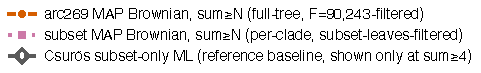
\includegraphics[width=0.92\linewidth,height=\textheight,keepaspectratio,alt={rate path legend}]{../validation/outputs/rate_path_min_legend.pdf}

The Csurös subset-only ML reference (gray ◇ dashed) is shown only at
min=4 since that's the only filter Csurös fits at.

\paragraph{Per-min rate paths (4 subset panels
each)}\label{per-min-rate-paths-4-subset-panels-each}

\texttt{min=4} is the canonical Csurös-matched comparison --- shown
first. Other min levels follow as filter-sensitivity diagnostics.

\textbf{min=4 --- canonical Csurös-matched (click to expand other mins)}

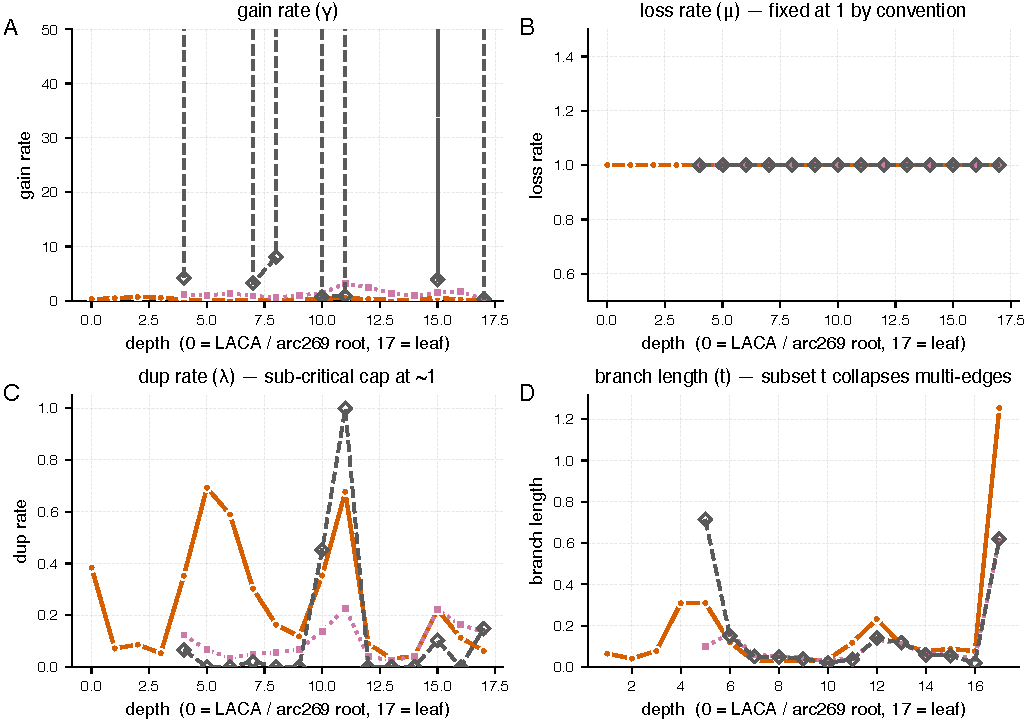
\includegraphics[width=0.92\linewidth,height=\textheight,keepaspectratio,alt={rate path min4 dpann80}]{../validation/outputs/rate_path_min4_dpann80.pdf}
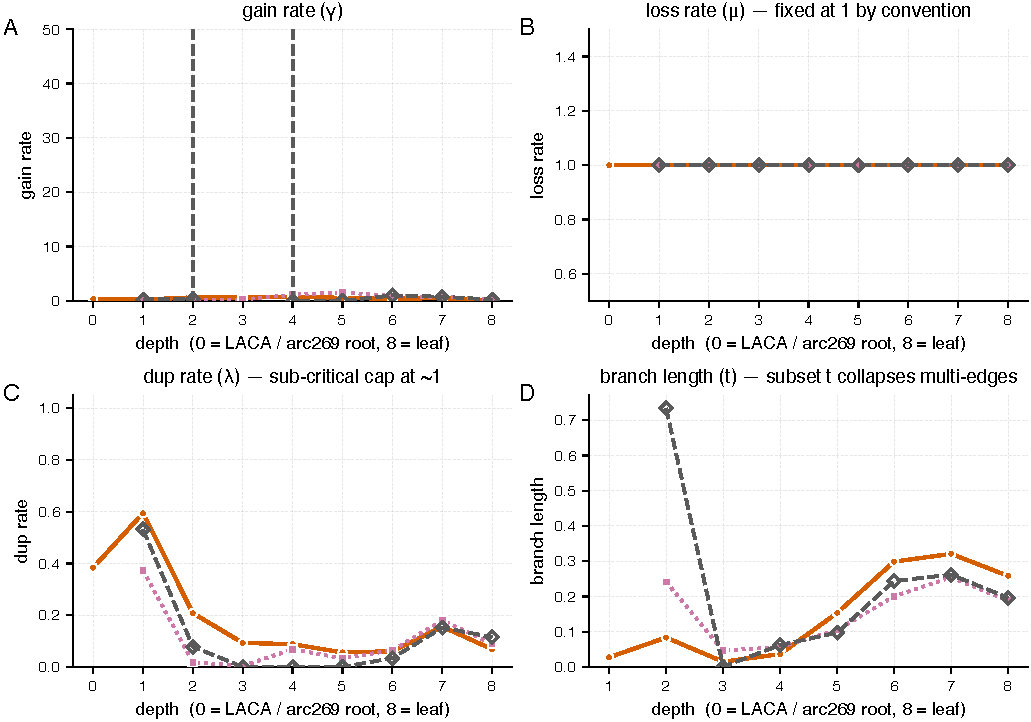
\includegraphics[width=0.92\linewidth,height=\textheight,keepaspectratio,alt={rate path min4 proteo75}]{../validation/outputs/rate_path_min4_proteo75.pdf}
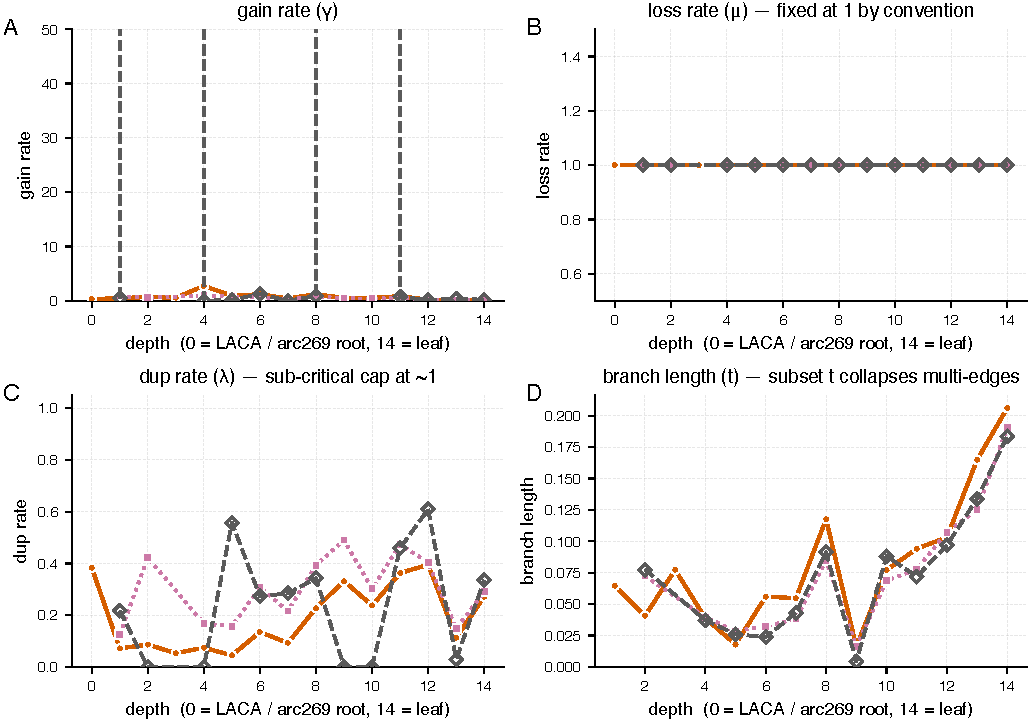
\includegraphics[width=0.92\linewidth,height=\textheight,keepaspectratio,alt={rate path min4 eury114}]{../validation/outputs/rate_path_min4_eury114.pdf}
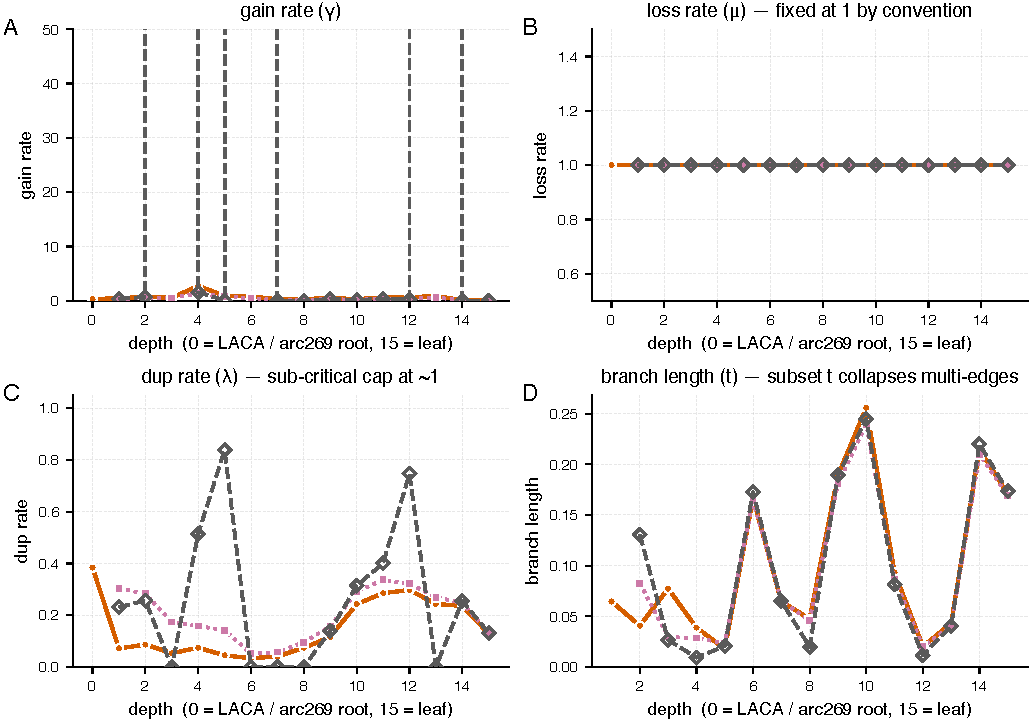
\includegraphics[width=0.92\linewidth,height=\textheight,keepaspectratio,alt={rate path min4 ed194}]{../validation/outputs/rate_path_min4_ed194.pdf}

\textbf{min=1 (no filter)}

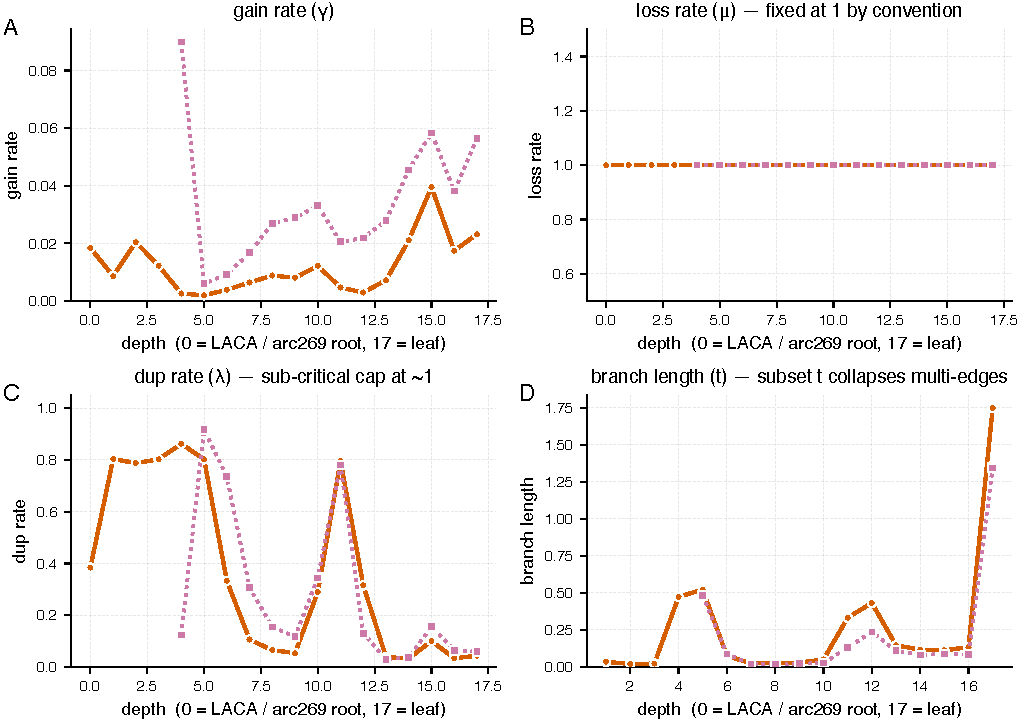
\includegraphics[width=0.92\linewidth,height=\textheight,keepaspectratio,alt={rate path min1 dpann80}]{../validation/outputs/rate_path_min1_dpann80.pdf}
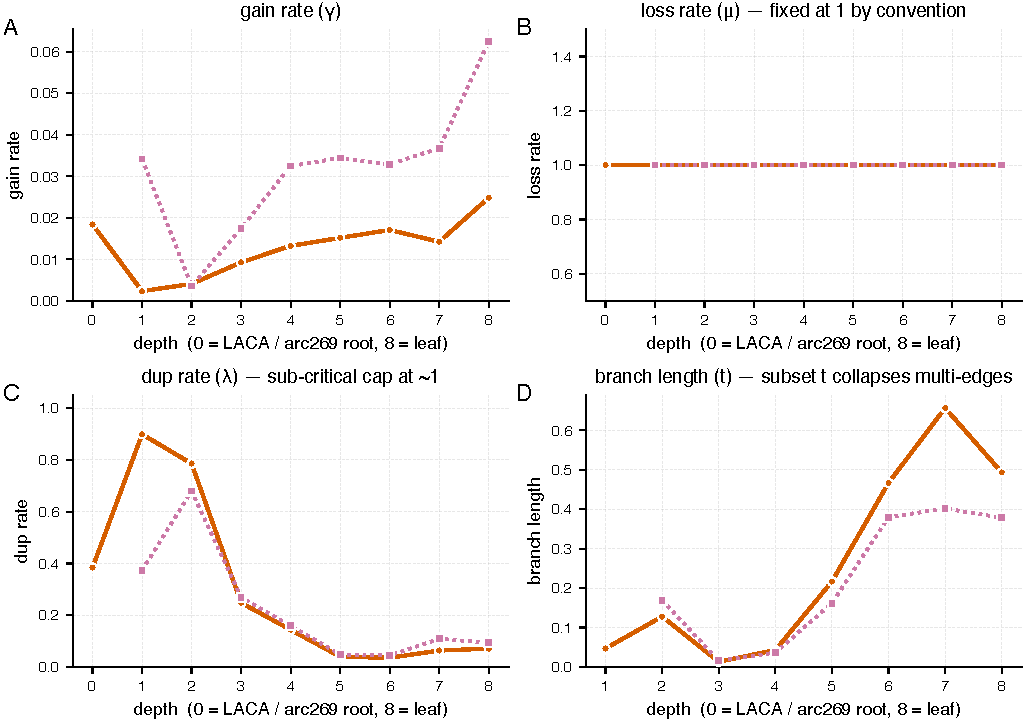
\includegraphics[width=0.92\linewidth,height=\textheight,keepaspectratio,alt={rate path min1 proteo75}]{../validation/outputs/rate_path_min1_proteo75.pdf}
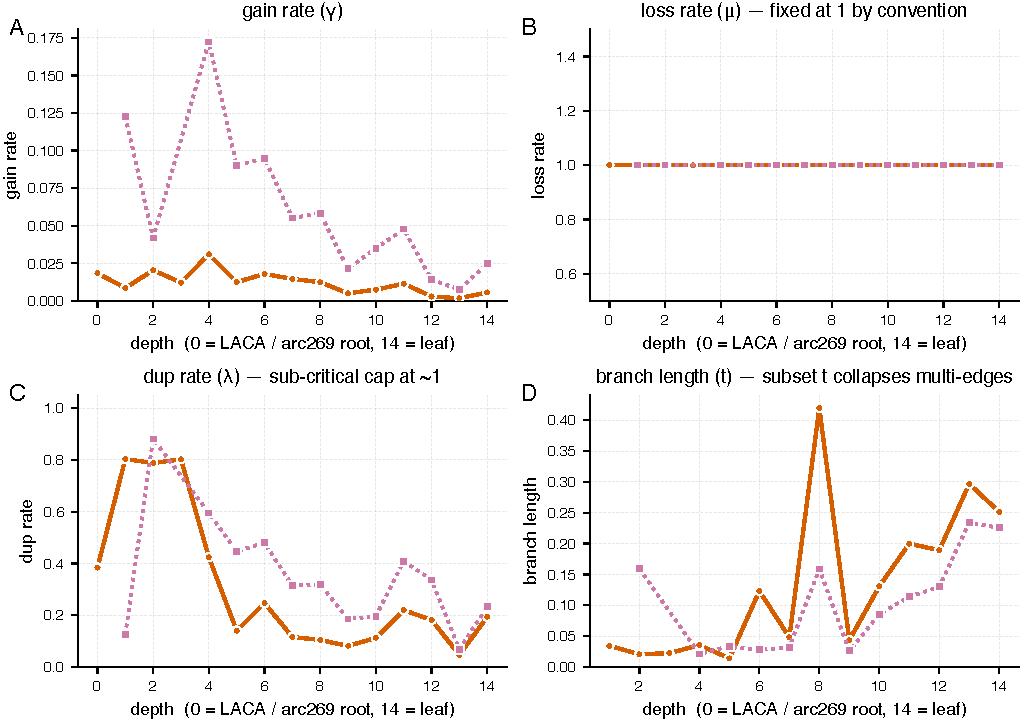
\includegraphics[width=0.92\linewidth,height=\textheight,keepaspectratio,alt={rate path min1 eury114}]{../validation/outputs/rate_path_min1_eury114.pdf}
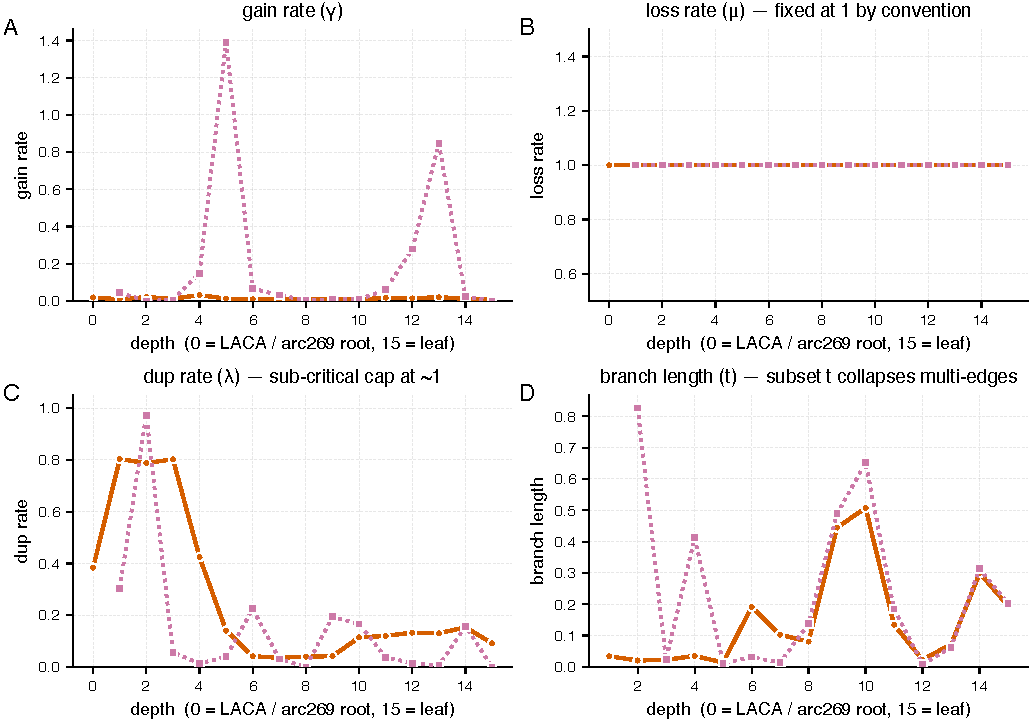
\includegraphics[width=0.92\linewidth,height=\textheight,keepaspectratio,alt={rate path min1 ed194}]{../validation/outputs/rate_path_min1_ed194.pdf}

\textbf{min=2}

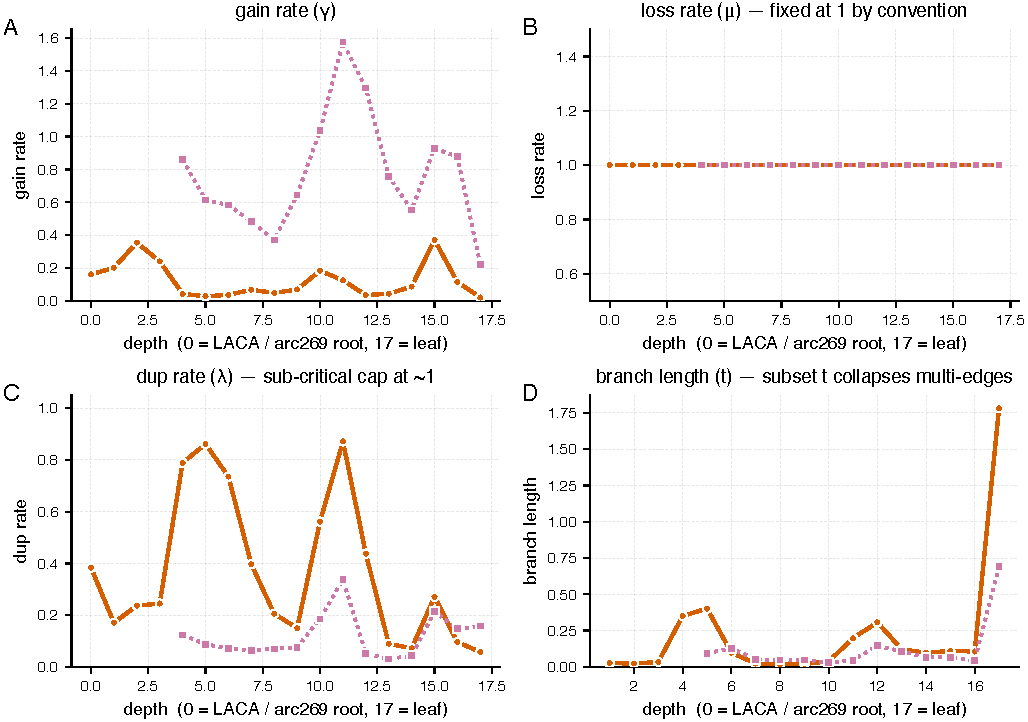
\includegraphics[width=0.92\linewidth,height=\textheight,keepaspectratio,alt={rate path min2 dpann80}]{../validation/outputs/rate_path_min2_dpann80.pdf}
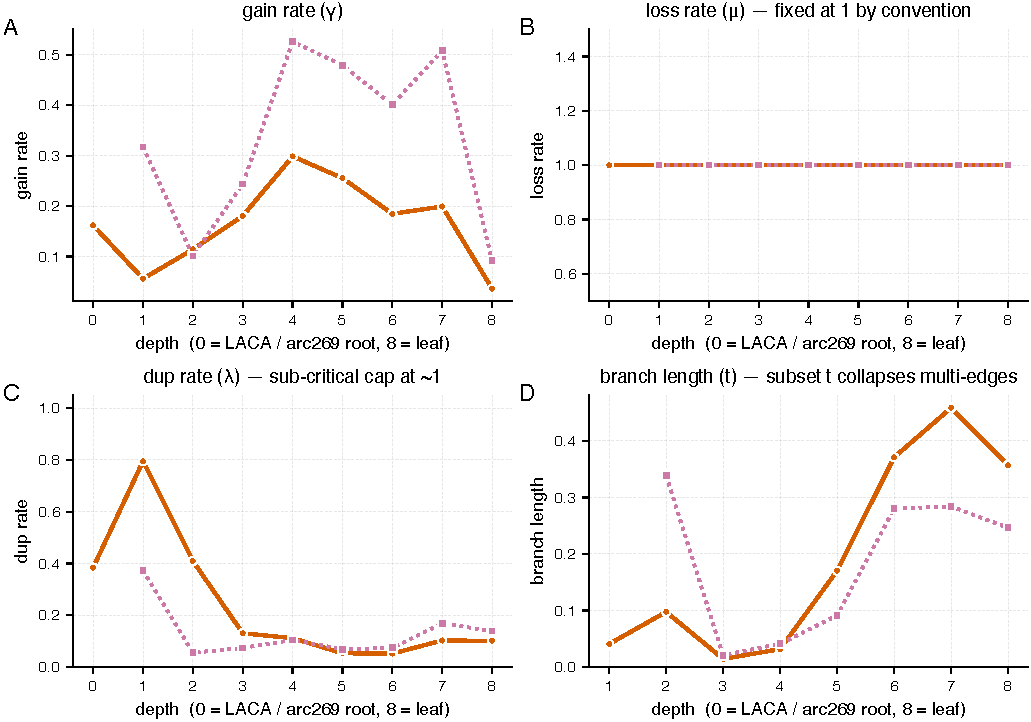
\includegraphics[width=0.92\linewidth,height=\textheight,keepaspectratio,alt={rate path min2 proteo75}]{../validation/outputs/rate_path_min2_proteo75.pdf}
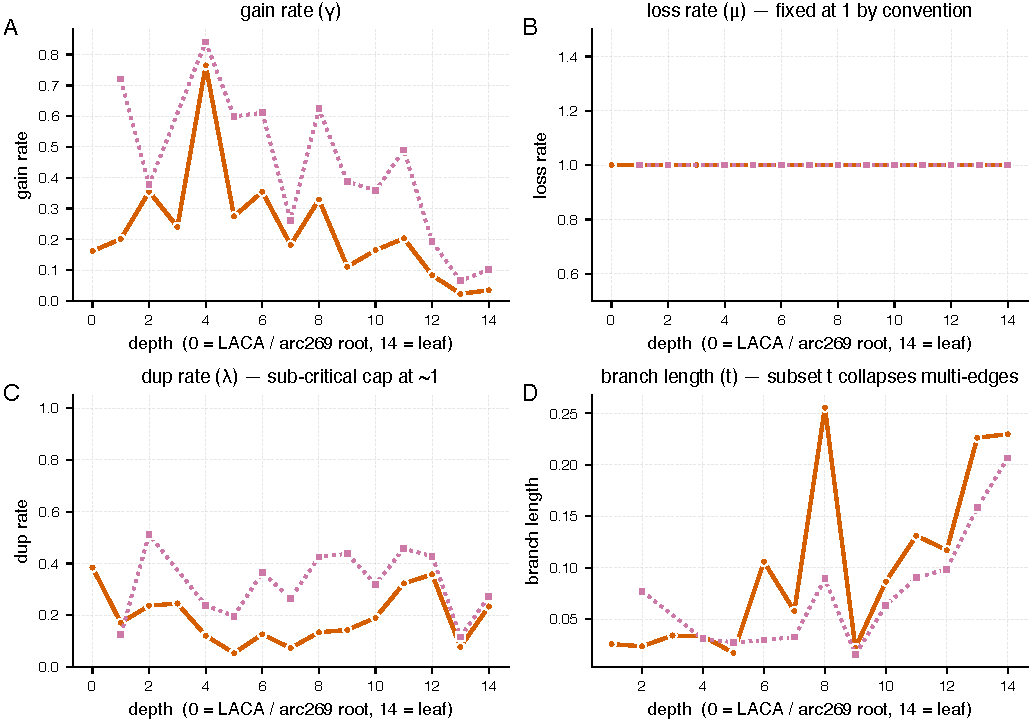
\includegraphics[width=0.92\linewidth,height=\textheight,keepaspectratio,alt={rate path min2 eury114}]{../validation/outputs/rate_path_min2_eury114.pdf}
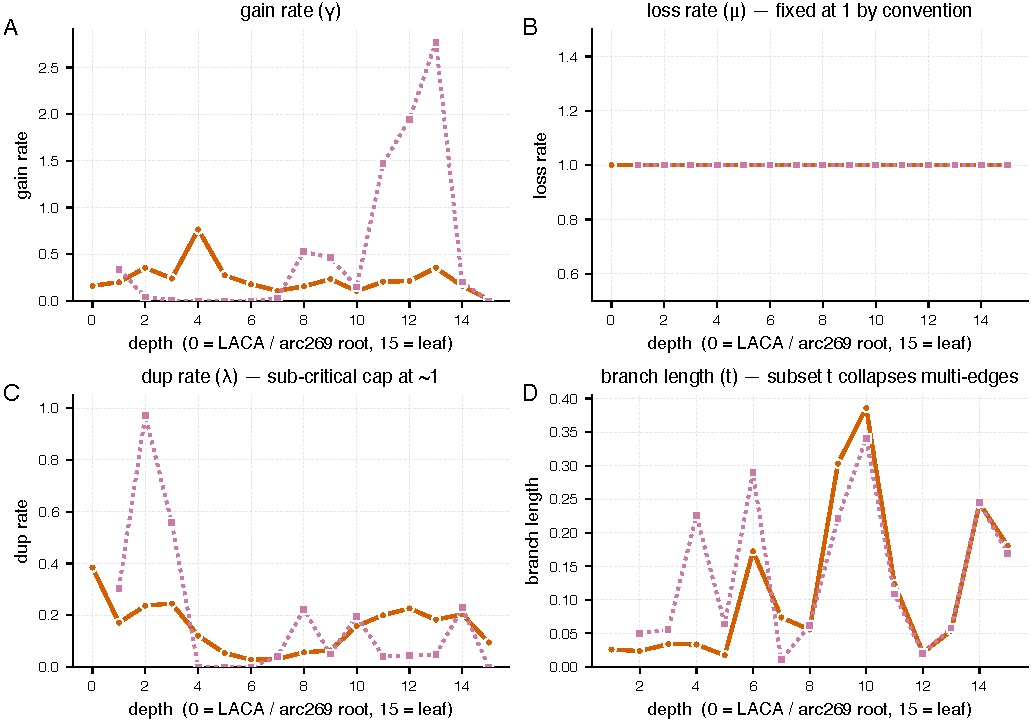
\includegraphics[width=0.92\linewidth,height=\textheight,keepaspectratio,alt={rate path min2 ed194}]{../validation/outputs/rate_path_min2_ed194.pdf}

\textbf{min=3}

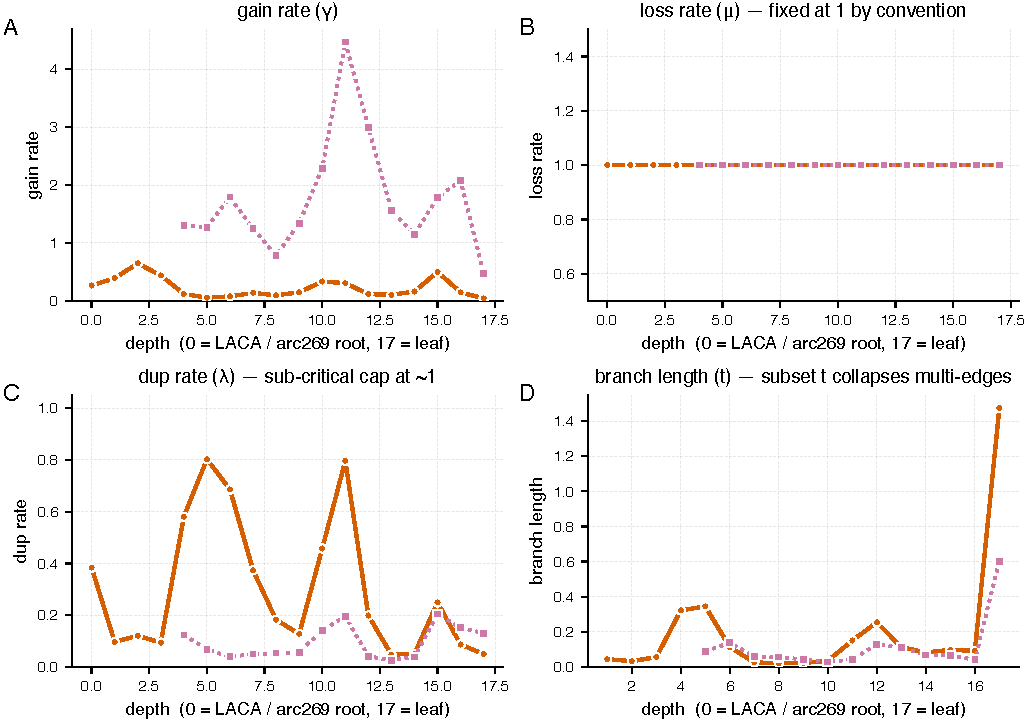
\includegraphics[width=0.92\linewidth,height=\textheight,keepaspectratio,alt={rate path min3 dpann80}]{../validation/outputs/rate_path_min3_dpann80.pdf}
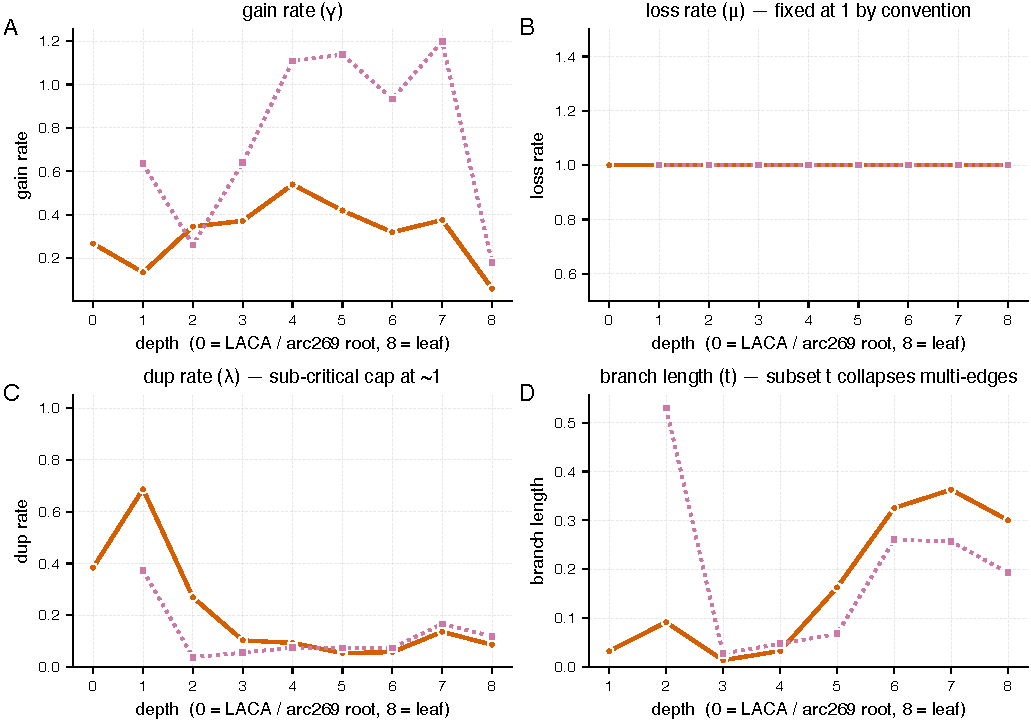
\includegraphics[width=0.92\linewidth,height=\textheight,keepaspectratio,alt={rate path min3 proteo75}]{../validation/outputs/rate_path_min3_proteo75.pdf}
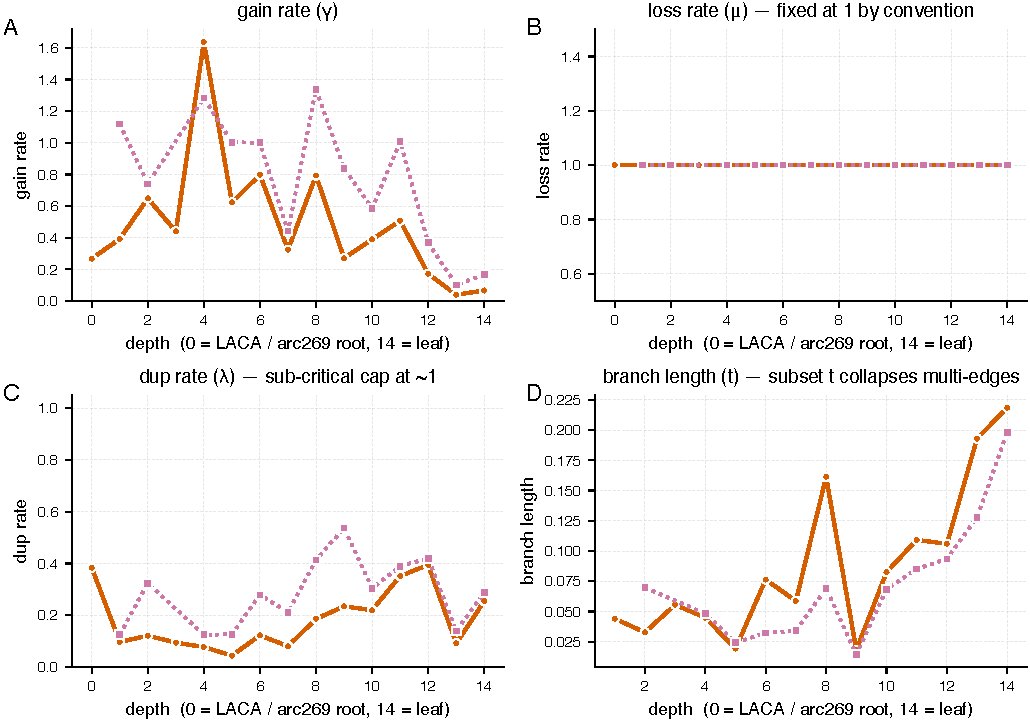
\includegraphics[width=0.92\linewidth,height=\textheight,keepaspectratio,alt={rate path min3 eury114}]{../validation/outputs/rate_path_min3_eury114.pdf}
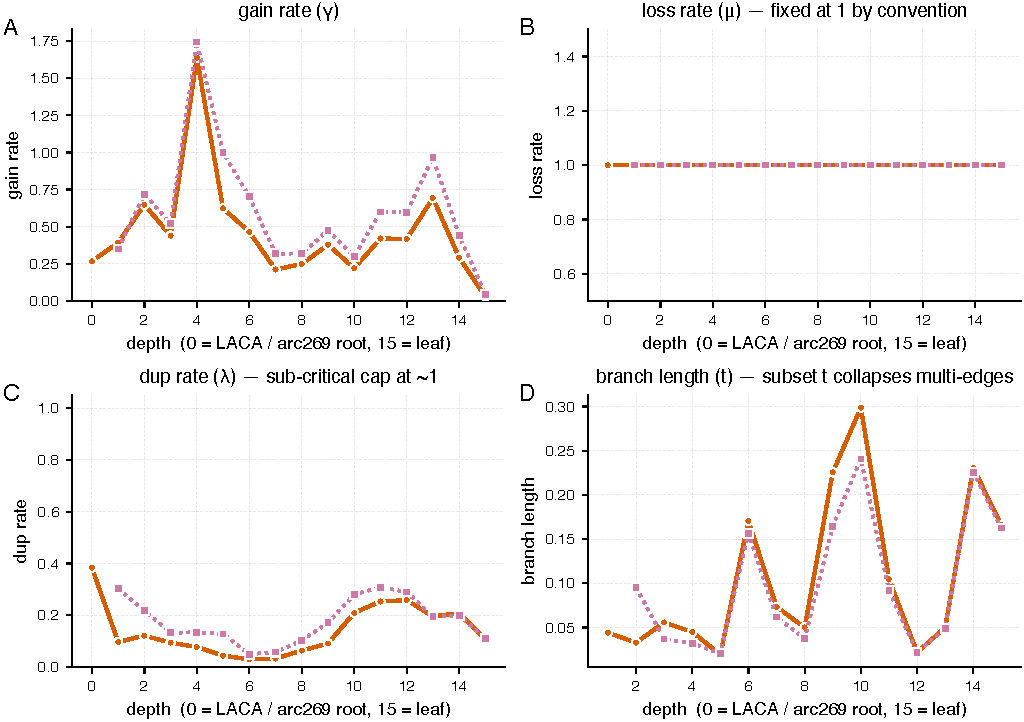
\includegraphics[width=0.92\linewidth,height=\textheight,keepaspectratio,alt={rate path min3 ed194}]{../validation/outputs/rate_path_min3_ed194.pdf}

\textbf{min=5}

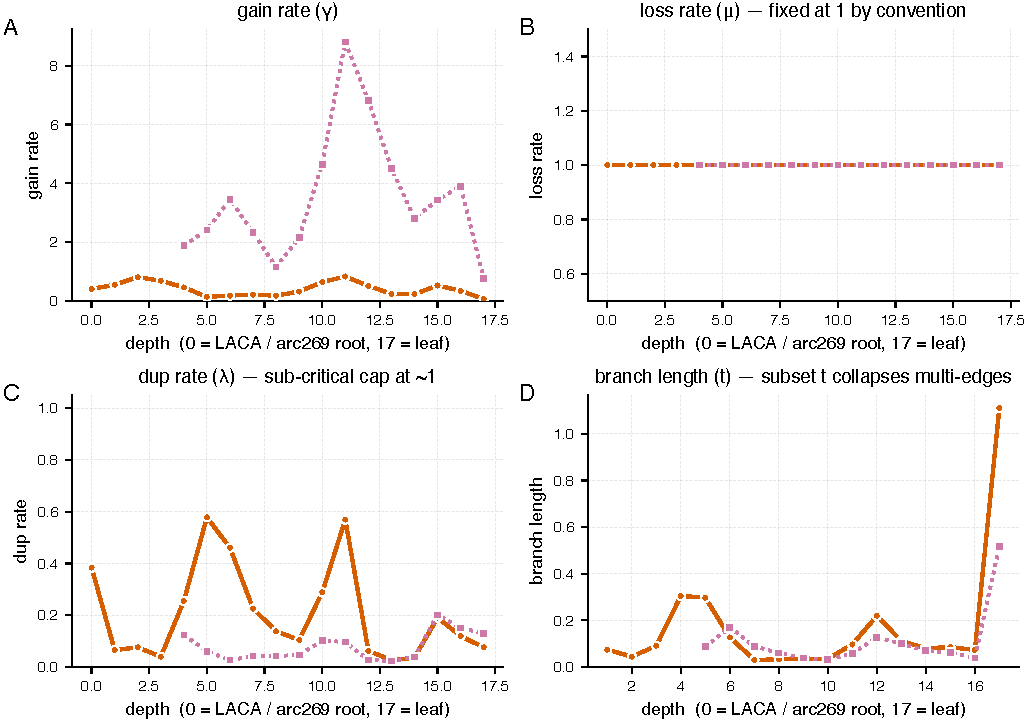
\includegraphics[width=0.92\linewidth,height=\textheight,keepaspectratio,alt={rate path min5 dpann80}]{../validation/outputs/rate_path_min5_dpann80.pdf}
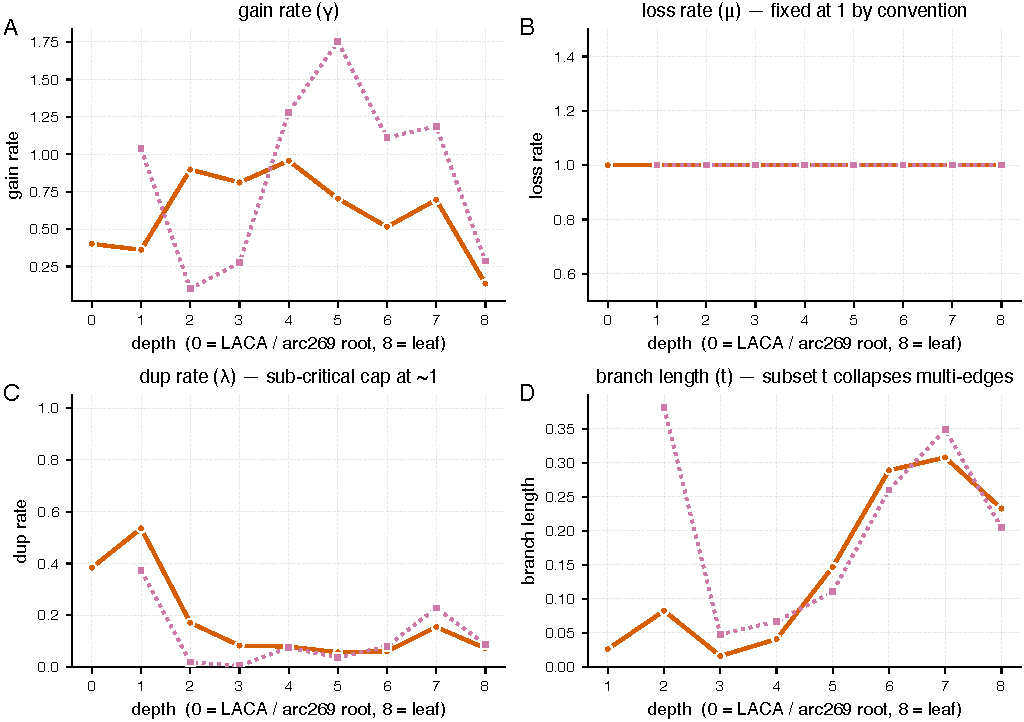
\includegraphics[width=0.92\linewidth,height=\textheight,keepaspectratio,alt={rate path min5 proteo75}]{../validation/outputs/rate_path_min5_proteo75.pdf}
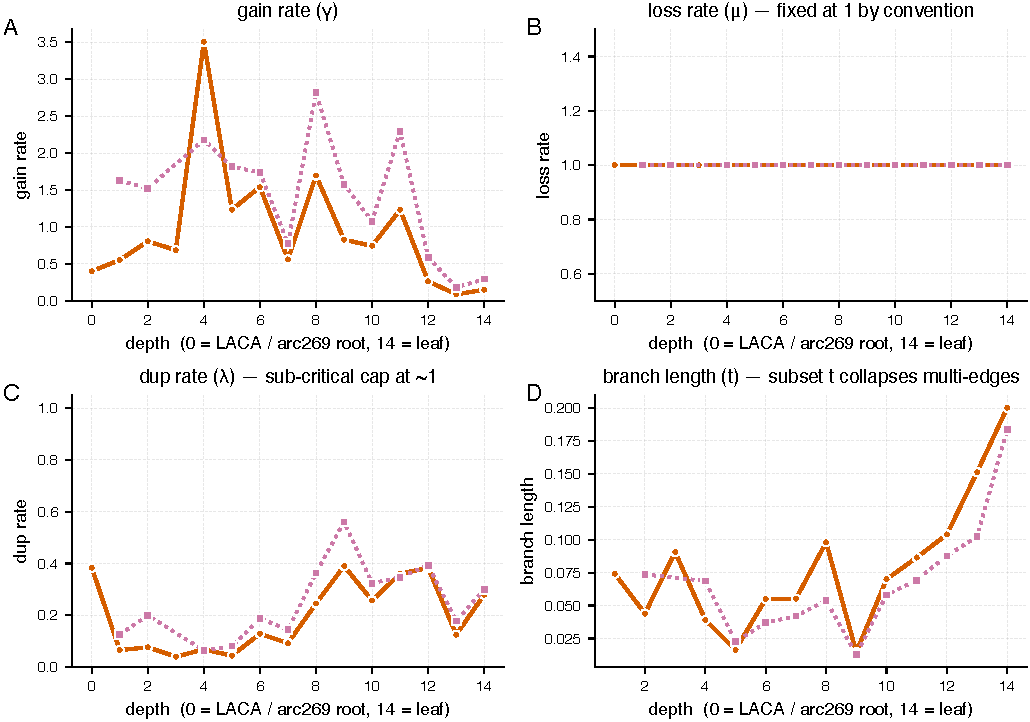
\includegraphics[width=0.92\linewidth,height=\textheight,keepaspectratio,alt={rate path min5 eury114}]{../validation/outputs/rate_path_min5_eury114.pdf}
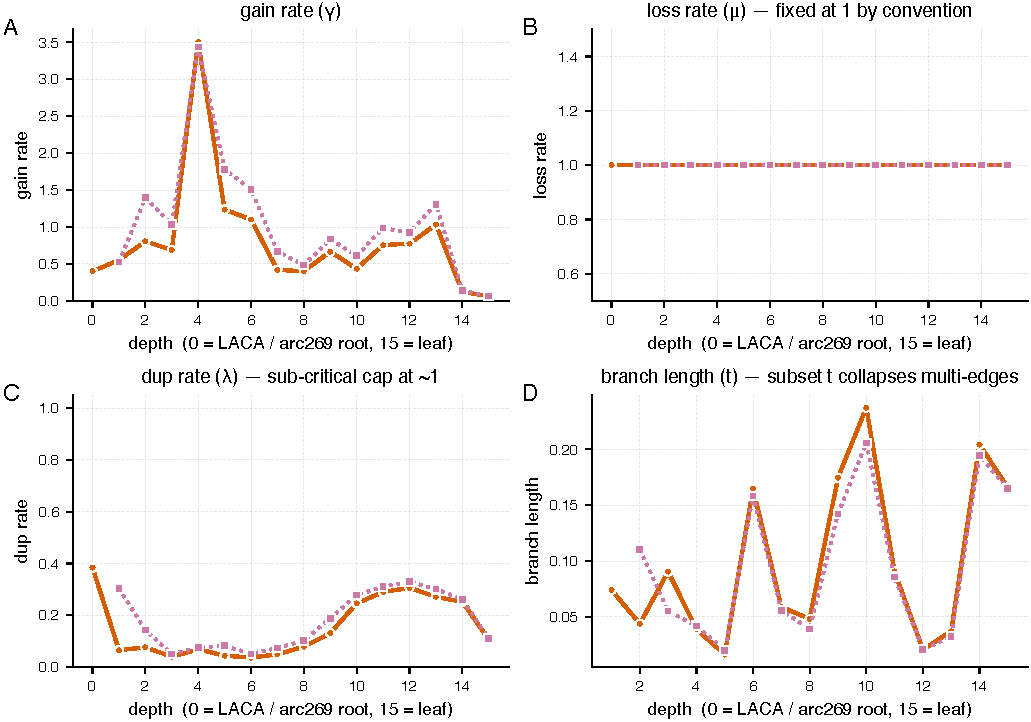
\includegraphics[width=0.92\linewidth,height=\textheight,keepaspectratio,alt={rate path min5 ed194}]{../validation/outputs/rate_path_min5_ed194.pdf}

\textbf{min=6}

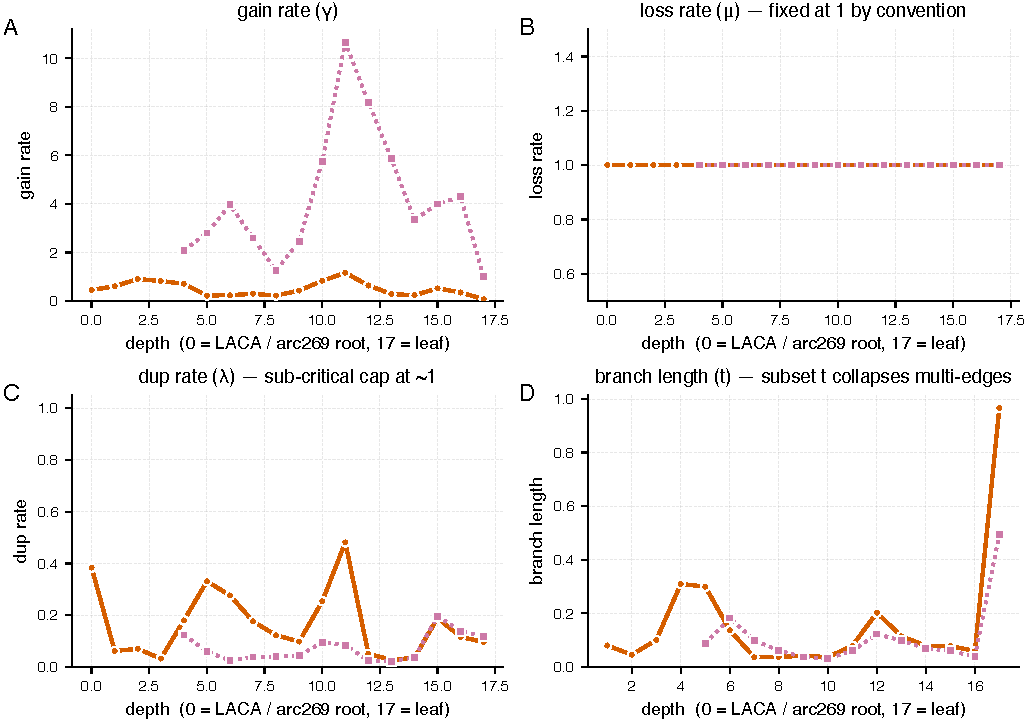
\includegraphics[width=0.92\linewidth,height=\textheight,keepaspectratio,alt={rate path min6 dpann80}]{../validation/outputs/rate_path_min6_dpann80.pdf}
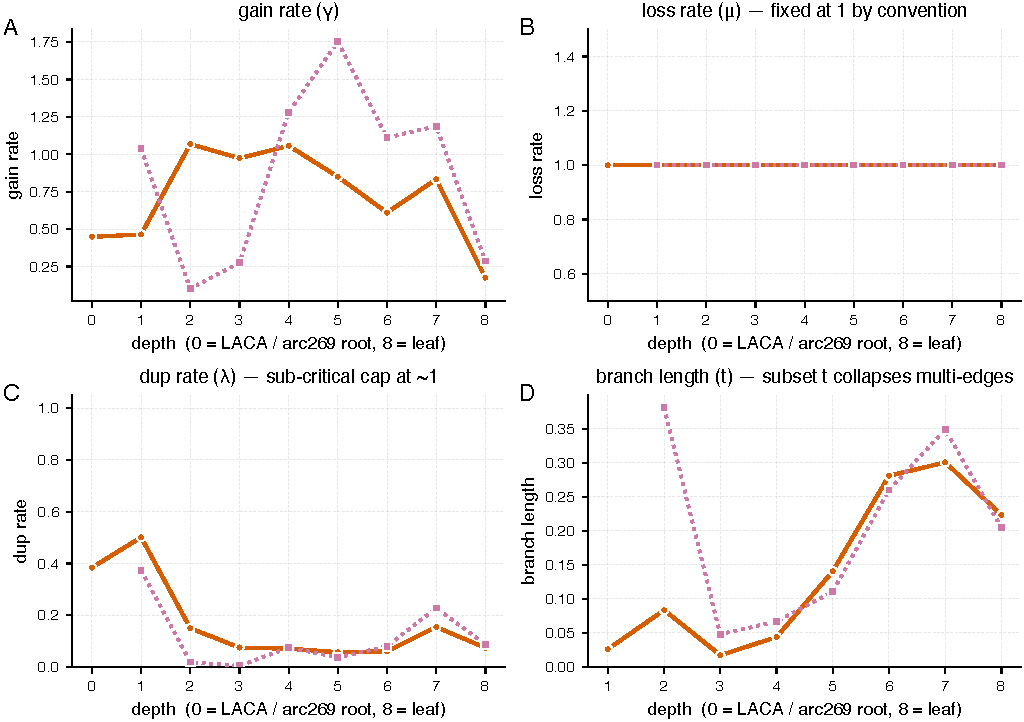
\includegraphics[width=0.92\linewidth,height=\textheight,keepaspectratio,alt={rate path min6 proteo75}]{../validation/outputs/rate_path_min6_proteo75.pdf}
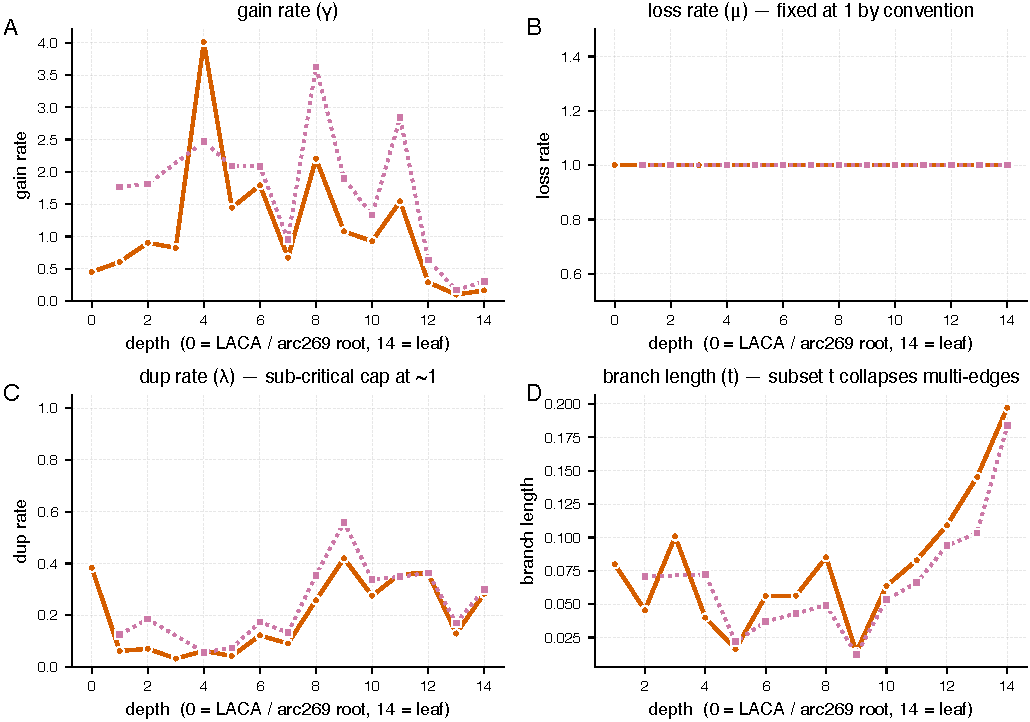
\includegraphics[width=0.92\linewidth,height=\textheight,keepaspectratio,alt={rate path min6 eury114}]{../validation/outputs/rate_path_min6_eury114.pdf}
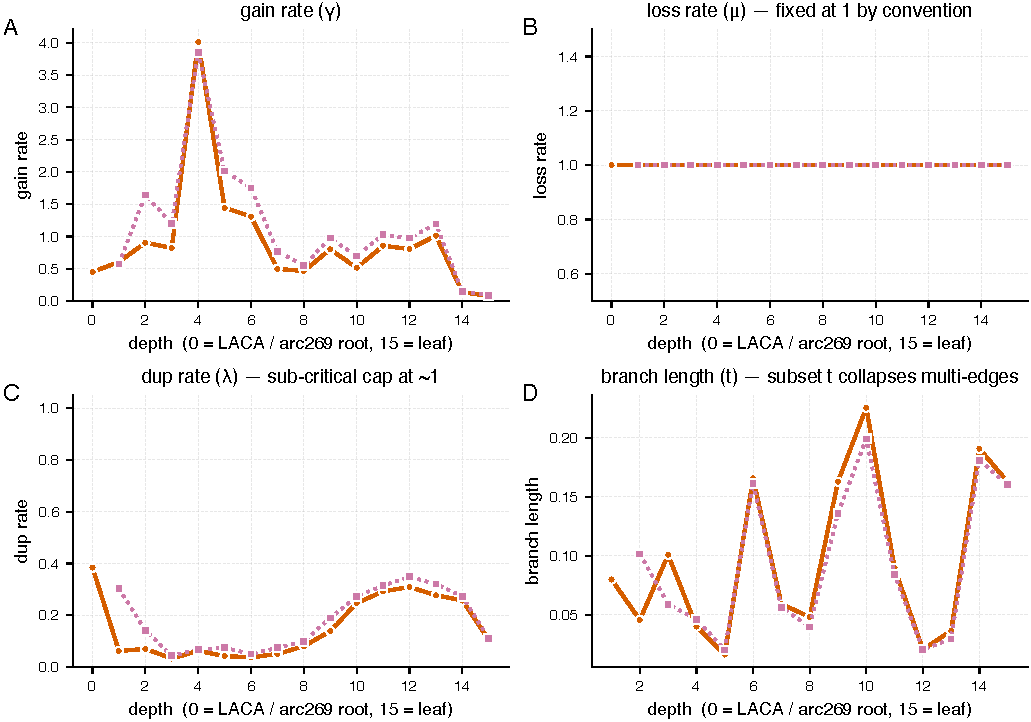
\includegraphics[width=0.92\linewidth,height=\textheight,keepaspectratio,alt={rate path min6 ed194}]{../validation/outputs/rate_path_min6_ed194.pdf}

\textbf{min=7 (most stringent)}

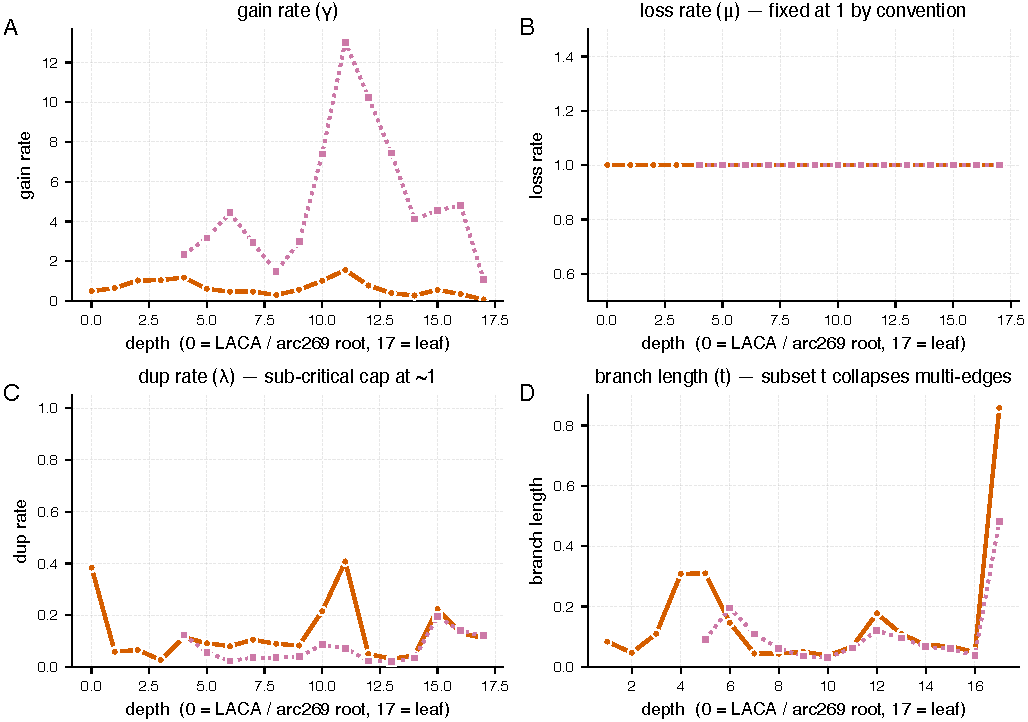
\includegraphics[width=0.92\linewidth,height=\textheight,keepaspectratio,alt={rate path min7 dpann80}]{../validation/outputs/rate_path_min7_dpann80.pdf}
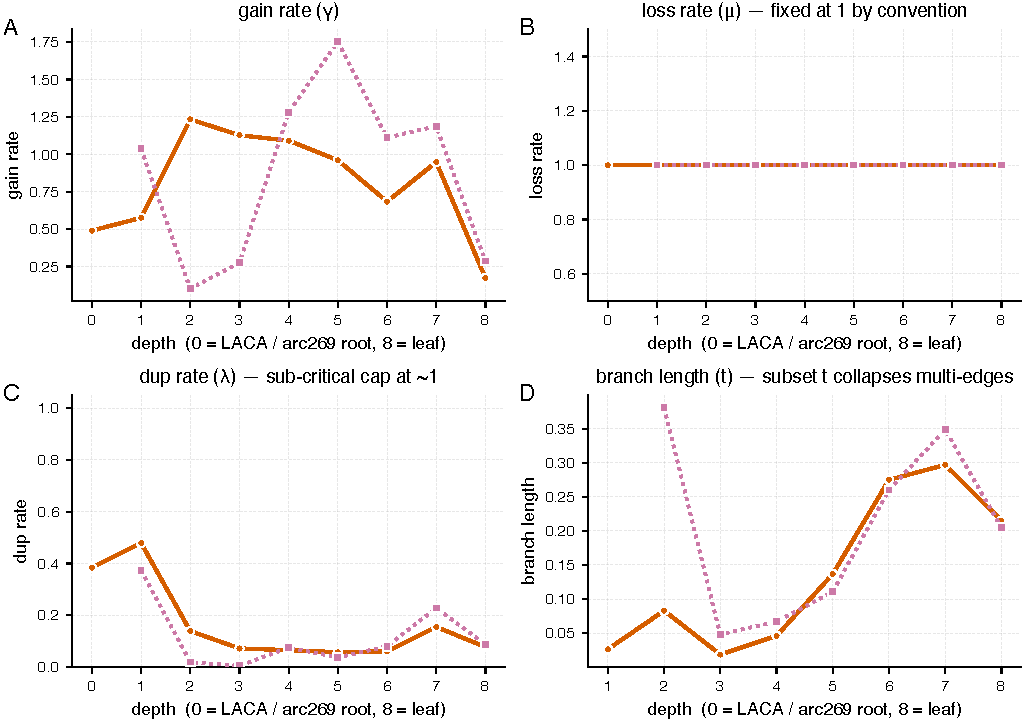
\includegraphics[width=0.92\linewidth,height=\textheight,keepaspectratio,alt={rate path min7 proteo75}]{../validation/outputs/rate_path_min7_proteo75.pdf}
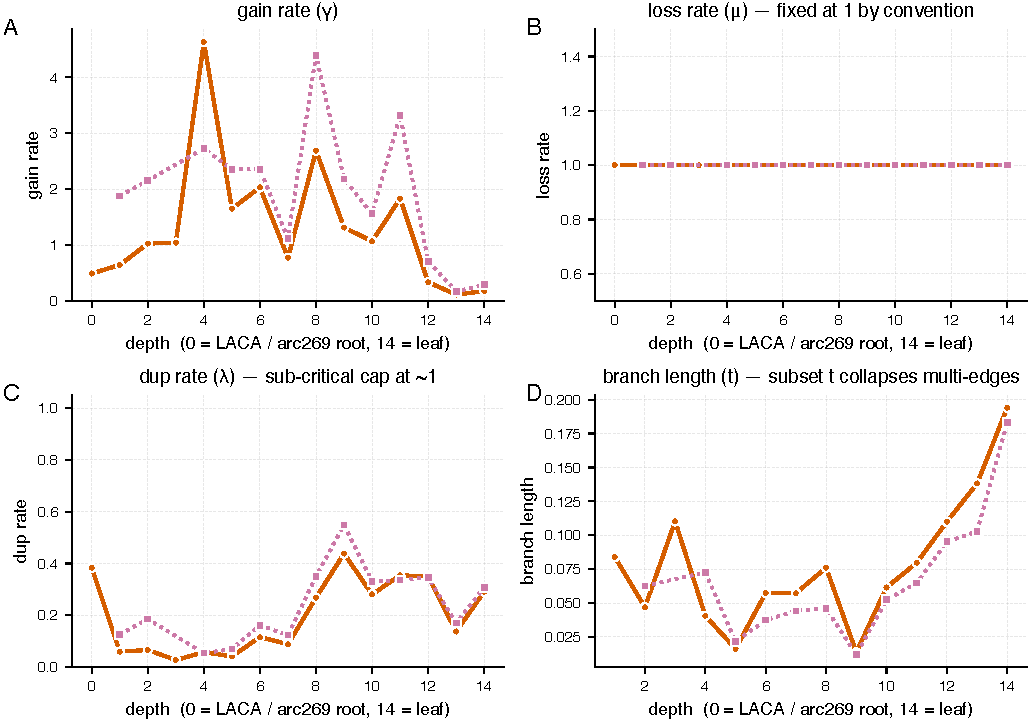
\includegraphics[width=0.92\linewidth,height=\textheight,keepaspectratio,alt={rate path min7 eury114}]{../validation/outputs/rate_path_min7_eury114.pdf}
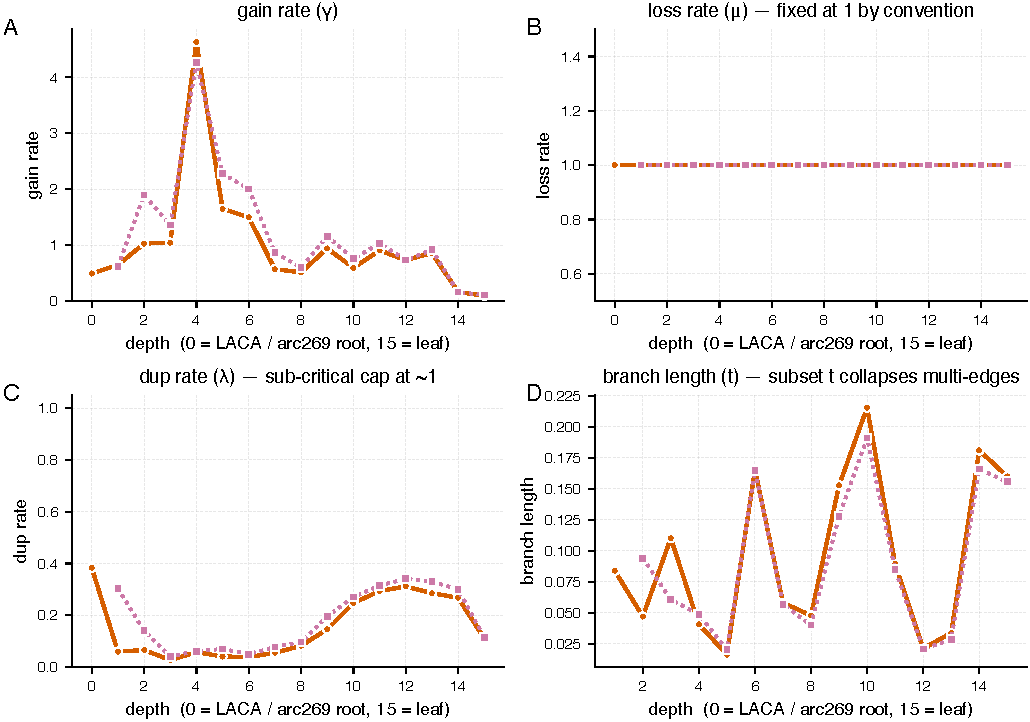
\includegraphics[width=0.92\linewidth,height=\textheight,keepaspectratio,alt={rate path min7 ed194}]{../validation/outputs/rate_path_min7_ed194.pdf}

\textbf{Figure 14.} Per-branch GLD rate paths (γ / μ / λ / t) along each
subset's root-to-leaf path, arc269 full-tree vs subset fit, at every
filter min N ∈ \{1..7\}.

\paragraph{Pooled per-branch rate scatter (across all 4 subsets, per
min)}\label{pooled-per-branch-rate-scatter-across-all-4-subsets-per-min}

Each marker is one LCA-matched internal-node triple; colour codes the
source subset (blue=dpann80, orange=proteo75, green=eury114, red=ed194).
Diagonal y=x is dashed black. Log axes on γ and t (heavy tails); linear
on λ (bounded sub-critical cap).

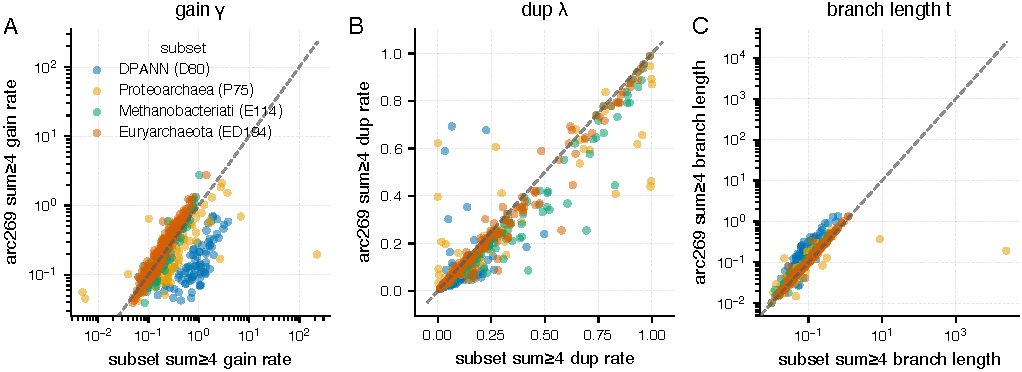
\includegraphics[width=0.92\linewidth,height=\textheight,keepaspectratio,alt={pooled rate scatter min4 (canonical)}]{../validation/outputs/rate_pooled_min4.pdf}

\textbf{Other min levels}

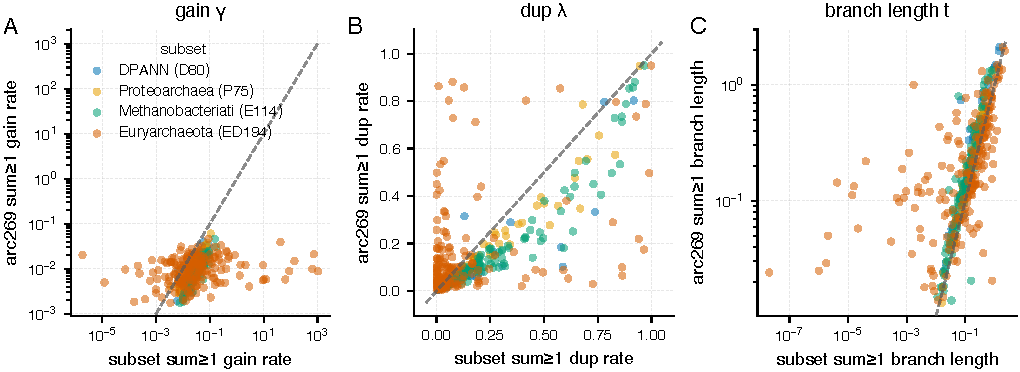
\includegraphics[width=0.92\linewidth,height=\textheight,keepaspectratio,alt={pooled rate scatter min1}]{../validation/outputs/rate_pooled_min1.pdf}
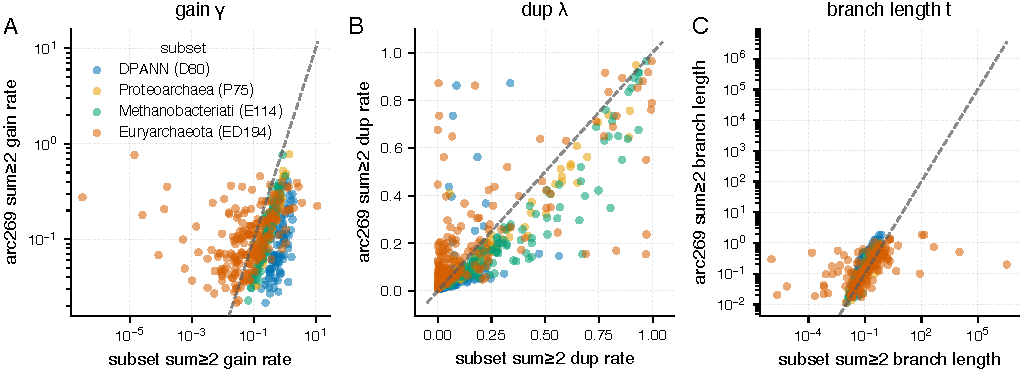
\includegraphics[width=0.92\linewidth,height=\textheight,keepaspectratio,alt={pooled rate scatter min2}]{../validation/outputs/rate_pooled_min2.pdf}
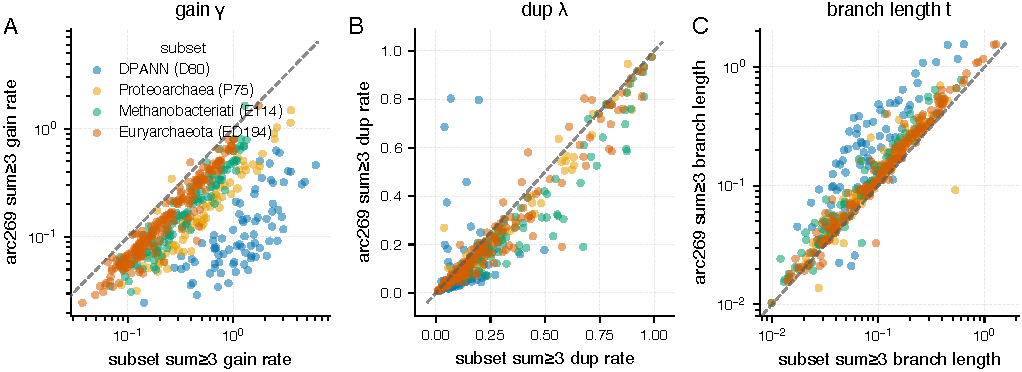
\includegraphics[width=0.92\linewidth,height=\textheight,keepaspectratio,alt={pooled rate scatter min3}]{../validation/outputs/rate_pooled_min3.pdf}
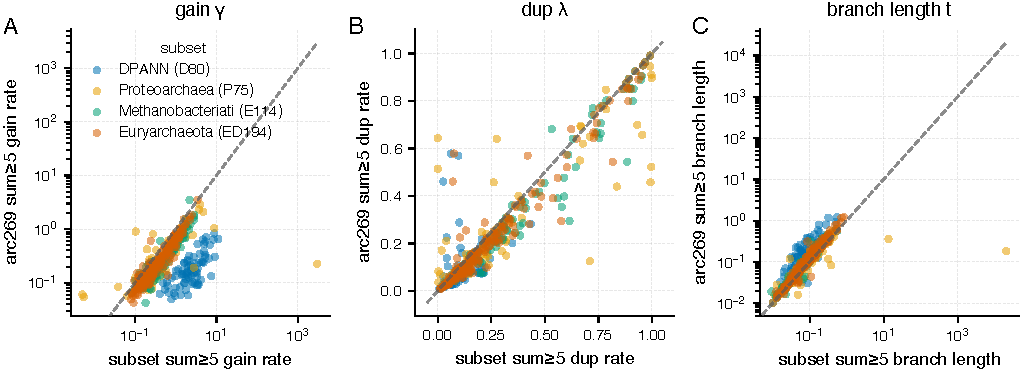
\includegraphics[width=0.92\linewidth,height=\textheight,keepaspectratio,alt={pooled rate scatter min5}]{../validation/outputs/rate_pooled_min5.pdf}
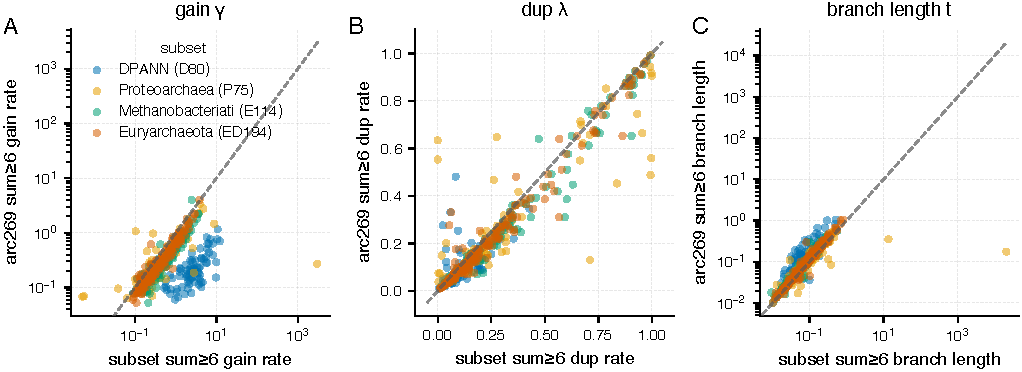
\includegraphics[width=0.92\linewidth,height=\textheight,keepaspectratio,alt={pooled rate scatter min6}]{../validation/outputs/rate_pooled_min6.pdf}
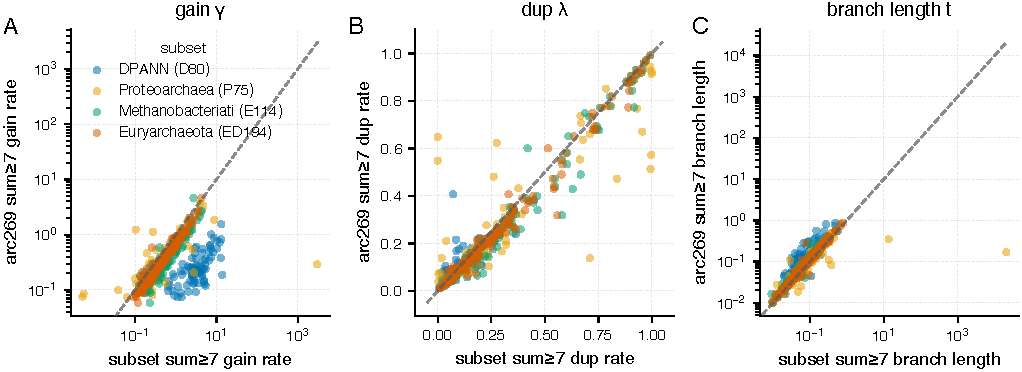
\includegraphics[width=0.92\linewidth,height=\textheight,keepaspectratio,alt={pooled rate scatter min7}]{../validation/outputs/rate_pooled_min7.pdf}

\textbf{Figure 15.} Pooled per-branch rate scatter (γ / λ / t) of arc269
vs subset rate at every LCA-matched internal node across all four
subsets, at each filter min N ∈ \{1..7\}.

\subsection{Performance}\label{performance}

\subsubsection{Single-core vs multi-thread on M4 Max (12 P + 4 E = 16
cores)}\label{single-core-vs-multi-thread-on-m4-max-12-p--4-e--16-cores}

Direct measurement on arc269 full-tree (F=90,243, N=537, mc=1 --- the
production case) at canonical rates (γ=λ=0.5, μ=1, t=1) on the
post-2026-05-19 fast kernel (commit \texttt{dc7653c}):

\textbf{Table 26.} Single-core vs multi-thread timings on arc269
full-tree (M4 Max, 16 cores).

\begin{center}
\begin{adjustbox}{max width=\textwidth}
\begin{tabular}{@{}rrrrr@{}}
\toprule\noalign{}
num\_threads & Forward LL & Gradient & Branch posteriors & Wall-time vs
1 thread \\
\midrule\noalign{}
1 & 2,257 ms & 5,523 ms & 5,529 ms & 1.00× \\
4 & 588 ms & 1,429 ms & 1,426 ms & 3.84× \\
16 (P + E) & 205 ms & 504 ms & 505 ms & 11.0× \\
\bottomrule\noalign{}
\end{tabular}
\end{adjustbox}
\end{center}

Near-linear up to 12 P-cores; the 4 E-cores add \textasciitilde15 \% on
top. Versus the pre-2026-05-19 kernel (commit \texttt{68e1bbe}, eury114
@ 8 threads): LL 890 ms → 205 ms, gradient 2,073 ms → 504 ms --- the
inside/outside refactor gives a 1.4--1.6× kernel-level speedup that
compounds with the parallelism.

\subsubsection{Speedup vs Csurös' Java reference (M4 Max, same
hardware)}\label{speedup-vs-csuruxf6s-java-reference-m4-max-same-hardware}

Direct measurement on Williams2017 (F=5,378, N=119, mc=4 --- Csurös'
canonical reference) plus two arc269 subsets, at canonical rates:

\textbf{Table 27.} Native (16-thread) vs Csurös' Java timings per
workload, with speedup, on the same M4 Max hardware.

\begin{center}
\begin{adjustbox}{max width=\textwidth}
\begin{tabular}{@{}lrrr@{}}
\toprule\noalign{}
Workload & Native (16-thread) & Java & Speedup \\
\midrule\noalign{}
Forward LL (Williams2017, F=5,378) & 9.5 ms & 227 ms & 24× \\
Branch posteriors (Williams2017) & 18.4 ms & 934 ms & 51× \\
Forward LL (arc269 halo51, F=256) & 1.2 ms & 36 ms & 30× \\
Forward LL (arc269 thermoplasmatota28) & 0.3 ms & 16 ms & 47× \\
Branch posteriors (arc269 halo51) & 2.4 ms & 197 ms & 81× \\
End-to-end MAP Brownian σ=1 (arc269, F=90,243) & \textasciitilde27 min &
\emph{Java cannot fit at -Xmx32g} & new mode \\
\bottomrule\noalign{}
\end{tabular}
\end{adjustbox}
\end{center}

Native runs eury114 (N=227, F=7,335, max W=712) and ed194 (N=387,
F=8,855, max W=712) in well under 100 ms per gradient call; Java cannot
complete either at −Xmx32g. arc269-subset comparisons reach 47× (LL) and
81× (branch posteriors) on sparser trees because libdispatch's
per-family parallelism scales better when per-family work is smaller.
Like-for-like comparison: same algorithm (Csurös 2021
\href{https://arxiv.org/abs/2107.11440}{arXiv v1} Theorem 11 ≡ Csurös
2022 TPB Theorem 12 + Csurös 2026 SI Thms 3--5), same hardware (M4 Max),
same numeric tolerance (≤ 5×10⁻¹¹ per-node).

Reproducible: \url{validation/benchmark_arc269_threads.py} and
\url{validation/benchmark_arc269_threads.json}.

\subsubsection{Threading scaling on Apple
silicon}\label{threading-scaling-on-apple-silicon}

\texttt{recount.native\_backend} parallelises per-family work via
libdispatch (Grand Central Dispatch). Default \texttt{num\_threads=0}
uses all online cores (P + E). Inspect the runtime topology:

\begin{Shaded}
\begin{Highlighting}[]
\OperatorTok{\textgreater{}\textgreater{}\textgreater{}} \ImportTok{from}\NormalTok{ recount.native\_backend }\ImportTok{import}\NormalTok{ cpu\_topology}
\OperatorTok{\textgreater{}\textgreater{}\textgreater{}}\NormalTok{ cpu\_topology()}
\NormalTok{\{}\StringTok{\textquotesingle{}ncpu\textquotesingle{}}\NormalTok{: }\DecValTok{16}\NormalTok{, }\StringTok{\textquotesingle{}physicalcpu\textquotesingle{}}\NormalTok{: }\DecValTok{16}\NormalTok{, }\StringTok{\textquotesingle{}perf\_cores\textquotesingle{}}\NormalTok{: }\DecValTok{12}\NormalTok{, }\StringTok{\textquotesingle{}eff\_cores\textquotesingle{}}\NormalTok{: }\DecValTok{4}\NormalTok{,}
 \StringTok{\textquotesingle{}brand\textquotesingle{}}\NormalTok{: }\StringTok{\textquotesingle{}Apple M4 Max\textquotesingle{}}\NormalTok{\}}
\end{Highlighting}
\end{Shaded}

The 4 E-cores add \textasciitilde10--15 \% on top of the 12 P-cores;
near-linear scaling up to 12 threads, slight diminishing returns past
that.

\subsection{Validation against Csurös'
Java}\label{validation-against-csuruxf6s-java}

Every numerical capability that the native C backend exposes is
validated against the bundled Java reference (\texttt{CountXXV.jar}):

\textbf{Table 28.} Each native C capability, its test against the Java
reference, and the agreement reached.

\begin{center}
\begin{adjustbox}{max width=\textwidth}
\begin{tabular}{@{}lll@{}}
\toprule\noalign{}
Capability & Test & Agreement \\
\midrule\noalign{}
Forward log-likelihood & \texttt{corrected\_log\_likelihood\_native} vs
Java on Williams2017 + 4 arc269 subsets & bit-for-bit, FP-sum floor ≈
5×10⁻¹⁰ \\
Family conditioning at arbitrary Ωmin (SI Thms 3--5) &
\texttt{unobserved\_logL0\_native} vs Java for Ωmin = 1, 2, 4 &
bit-for-bit, ≤ 1 ULP \\
Per-branch posterior copies \& families (observed) &
\texttt{per\_branch\_stats\_native} vs Java for all 4 focal subset
clades & ≤ 5×10⁻¹¹ at every per-node value \\
L(0)-corrected root copies \& families & end-to-end including the F ·
L(0)/(1−L(0)) amplification at Ωmin ≥ 2 & ≤ 5×10⁻¹¹ \\
Analytical survival-rate gradient & \texttt{gradient\_native} vs central
finite-difference, Williams + all 4 subsets & median 1×10⁻⁹ relative,
FP-sum floor ≈ 1×10⁻⁷ \\
Analytical L(0) gradient (Phase B) &
\texttt{compute\_L0\_gradient\_analytical} vs finite-difference for Ωmin
= 2, 4 & median 1×10⁻⁷ relative \\
LogisticShift K = 1, zero shifts & mixture LL identity collapses to
base-GLD LL & exact, diff = 0.0 \\
Brownian-prior gradient & \texttt{brownian\_prior\_native} vs central
finite-difference & max rel ≤ 10⁻⁶ \\
\bottomrule\noalign{}
\end{tabular}
\end{adjustbox}
\end{center}

See \url{VALIDATION.md} and \url{VALIDATION_FOCAL.md} §3 for per-node
diff dumps. The pytest suite (\texttt{pytest\ tests/}) re-runs every
check above in \textasciitilde2 s.

\subsubsection{Reproduction accuracy on the focal subset
clades}\label{reproduction-accuracy-on-the-focal-subset-clades}

Loading the bundled \texttt{.countxml.gz} rates from Csurös 2026 and
recomputing per-branch posteriors via the C backend matches the Java
output from \href{https://github.com/miklosc/Count}{miklosc/Count} to ≤
5×10⁻¹¹ at every per-node copy/family/event count:

\textbf{Table 29.} Per-node reproduction accuracy vs Java for each focal
subset clade and Williams2017.

\begin{center}
\begin{adjustbox}{max width=\textwidth}
\begin{tabular}{@{}lrrrr@{}}
\toprule\noalign{}
Dataset & F families & leaves & nodes & per-node max diff vs Java \\
\midrule\noalign{}
DPANN (D80) & 3,034 & 80 & 159 & ≤ 5×10⁻¹¹ \\
Proteoarchaea (P75) & 5,179 & 75 & 149 & ≤ 5×10⁻¹¹ \\
Methanobacteriati (E114) & 7,335 & 114 & 227 & ≤ 5×10⁻¹¹ \\
Euryarchaeota (ED194) & 8,855 & 194 & 387 & ≤ 5×10⁻¹¹ \\
Williams2017 (LACA) & 5,378 & 60 & 119 & ≤ 5×10⁻¹¹ \\
\bottomrule\noalign{}
\end{tabular}
\end{adjustbox}
\end{center}

\subsection{Repository tour}\label{repository-tour}

\begin{verbatim}
recount/                 # Python package
  gld.py                 # NumPy reference (forward + outside + gradient)
  torch_backend.py       # PyTorch reference (forward + autograd grad)
  native_backend.py      # production: ctypes wrappers for the native C dylib
  ml.py / logistic_shift.py / brownian_prior_*.py
native/                  # C backend (Apple Accelerate vForce + libdispatch)
  src/                   # forward, outside, gradient, brownian_prior, …
  include/               # public + internal headers
  test/                  # standalone C test (test_4leaf)
  Makefile               # auto-detects Apple Silicon / Intel Mac / Linux
validation/              # one-shot drivers + canonical queue + plot pipeline
  ml.py / map.py / brownian_extend_ml.py
  queue_full_subset_run.sh + QUEUE_INSTRUCTIONS.md
  reproduce.py           # Csurös' published rates → bit-perfect per-node check
  subclade_ancestor_comparison.py / brownian_split_path_plots.py / …
  outputs/<fit-dir>/<ds>_{branches.csv, countxml.gz, summary.json, final_rates.npz}
docs/                    # specifications, proofs, and the PDF build
  brownian_prior.tex     # TKP autocorrelated-rate prior + gradient derivation
  boundary_identifiability.tex
  PER_FAMILY_PRESENCE.md
  build_readme_pdf.py    # regenerates README.{tex,pdf} from README.md
  README.tex / README.pdf  # LaTeX / PDF rendering of this README (generated)
tests/                   # pytest (~30 checks)
\end{verbatim}

A typeset LaTeX/PDF version of this README is kept at
\url{docs/README.pdf}. It is generated, not hand-written: after editing
\texttt{README.md}, run \texttt{python3\ docs/build\_readme\_pdf.py} to
rebuild \texttt{docs/README.tex} and \texttt{docs/README.pdf} (the build
uses the vector PDF version of every plot). That keeps the two in sync
--- the Markdown README is always the source of truth.

\subsection{Per-family per-node presence
tables}\label{per-family-per-node-presence-tables}

For any saved fit, you can produce two F × N matrices on demand:

\textbf{Table 30.} The two per-family per-node F × N matrices a saved
fit can produce, with each element's meaning.

\begin{center}
\begin{adjustbox}{max width=\textwidth}
\begin{tabular}{@{}lll@{}}
\toprule\noalign{}
matrix & element & meaning \\
\midrule\noalign{}
\texttt{present{[}f,\ v{]}} & P\{ ξ\_v ≥ 1 given data\_f, fitted rates
\} & posterior probability family \emph{f} is present at node
\emph{v} \\
\texttt{copies{[}f,\ v{]}} & E{[} ξ\_v given data\_f, fitted rates {]} &
posterior expected copy number for \emph{f} at \emph{v} \\
\bottomrule\noalign{}
\end{tabular}
\end{adjustbox}
\end{center}

These are intentionally \textbf{not} written by the standard fit
pipelines (F × N is heavy on disk --- arc269 is \textasciitilde21 MB
compressed NPZ per matrix). Generate explicitly:

\begin{Shaded}
\begin{Highlighting}[]
\CommentTok{\# Compute for every dataset whose rates are present in a fit directory:}
\VariableTok{PYTHONPATH}\OperatorTok{=}\NormalTok{. }\ExtensionTok{python3}\NormalTok{ validation/per\_family\_presence.py }\AttributeTok{{-}{-}all} \DataTypeTok{\textbackslash{}}
    \AttributeTok{{-}{-}fit{-}dir}\NormalTok{ validation/outputs/brownian\_arc269}
\end{Highlighting}
\end{Shaded}

Recipe + query patterns: \url{docs/PER_FAMILY_PRESENCE.md}.

\subsection{Low-level Python API}\label{low-level-python-api}

For research / scripting, build a tree + rates by hand:

\begin{Shaded}
\begin{Highlighting}[]
\ImportTok{import}\NormalTok{ numpy }\ImportTok{as}\NormalTok{ np}
\ImportTok{from}\NormalTok{ recount }\ImportTok{import}\NormalTok{ Tree, GLDRates, corrected\_log\_likelihood, gradient\_survival}

\CommentTok{\# Tree: ((A:0.5,B:0.3):0.2,(C:0.4,D:0.6):0.1);}
\CommentTok{\# Indexing: leaves first, parent index \textgreater{} child index, root has parent {-}1.}
\NormalTok{tree }\OperatorTok{=}\NormalTok{ Tree(parent}\OperatorTok{=}\NormalTok{np.array([}\DecValTok{4}\NormalTok{, }\DecValTok{4}\NormalTok{, }\DecValTok{5}\NormalTok{, }\DecValTok{5}\NormalTok{, }\DecValTok{6}\NormalTok{, }\DecValTok{6}\NormalTok{, }\OperatorTok{{-}}\DecValTok{1}\NormalTok{]),}
\NormalTok{            leaf\_names}\OperatorTok{=}\NormalTok{[}\StringTok{"A"}\NormalTok{, }\StringTok{"B"}\NormalTok{, }\StringTok{"C"}\NormalTok{, }\StringTok{"D"}\NormalTok{])}

\NormalTok{rates }\OperatorTok{=}\NormalTok{ GLDRates(}
\NormalTok{    tree}\OperatorTok{=}\NormalTok{tree,}
\NormalTok{    gain   }\OperatorTok{=}\NormalTok{ np.array([}\FloatTok{0.10}\NormalTok{, }\FloatTok{0.20}\NormalTok{, }\FloatTok{0.15}\NormalTok{, }\FloatTok{0.25}\NormalTok{, }\FloatTok{0.30}\NormalTok{, }\FloatTok{0.18}\NormalTok{, }\FloatTok{0.50}\NormalTok{]),}
\NormalTok{    loss   }\OperatorTok{=}\NormalTok{ np.array([}\FloatTok{1.00}\NormalTok{] }\OperatorTok{*} \DecValTok{7}\NormalTok{),}
\NormalTok{    dup    }\OperatorTok{=}\NormalTok{ np.array([}\FloatTok{0.40}\NormalTok{, }\FloatTok{0.30}\NormalTok{, }\FloatTok{0.50}\NormalTok{, }\FloatTok{0.20}\NormalTok{, }\FloatTok{0.45}\NormalTok{, }\FloatTok{0.35}\NormalTok{, }\FloatTok{0.00}\NormalTok{]),}
\NormalTok{    length }\OperatorTok{=}\NormalTok{ np.array([}\FloatTok{0.50}\NormalTok{, }\FloatTok{0.30}\NormalTok{, }\FloatTok{0.40}\NormalTok{, }\FloatTok{0.60}\NormalTok{, }\FloatTok{0.20}\NormalTok{, }\FloatTok{0.10}\NormalTok{, np.inf]),}
\NormalTok{)}
\NormalTok{profiles }\OperatorTok{=}\NormalTok{ np.array([}
\NormalTok{    [}\DecValTok{1}\NormalTok{, }\DecValTok{0}\NormalTok{, }\DecValTok{1}\NormalTok{, }\DecValTok{1}\NormalTok{],}
\NormalTok{    [}\DecValTok{2}\NormalTok{, }\DecValTok{0}\NormalTok{, }\DecValTok{0}\NormalTok{, }\DecValTok{1}\NormalTok{],}
\NormalTok{    [}\DecValTok{1}\NormalTok{, }\DecValTok{1}\NormalTok{, }\DecValTok{1}\NormalTok{, }\DecValTok{1}\NormalTok{],}
\NormalTok{    [}\DecValTok{3}\NormalTok{, }\DecValTok{2}\NormalTok{, }\DecValTok{1}\NormalTok{, }\DecValTok{0}\NormalTok{],}
\NormalTok{], dtype}\OperatorTok{=}\NormalTok{np.int64)}

\NormalTok{ll }\OperatorTok{=}\NormalTok{ corrected\_log\_likelihood(tree, rates, profiles, min\_copies}\OperatorTok{=}\DecValTok{1}\NormalTok{)}
\NormalTok{g  }\OperatorTok{=}\NormalTok{ gradient\_survival(tree, rates, profiles, min\_copies}\OperatorTok{=}\DecValTok{1}\NormalTok{)}
\CommentTok{\# g has shape (3 * num\_nodes,), indexed as 3*v + \{GAIN=0, LOSS=1, DUP=2\}}
\end{Highlighting}
\end{Shaded}

PyTorch path (autograd through \texttt{compute\_survival\_params\_t}):

\begin{Shaded}
\begin{Highlighting}[]
\ImportTok{import}\NormalTok{ torch}
\ImportTok{from}\NormalTok{ recount.torch\_backend }\ImportTok{import}\NormalTok{ corrected\_log\_likelihood\_t, gradient\_autograd}

\NormalTok{dt }\OperatorTok{=}\NormalTok{ torch.float64}
\NormalTok{gain   }\OperatorTok{=}\NormalTok{ torch.tensor([}\FloatTok{0.10}\NormalTok{, }\FloatTok{0.20}\NormalTok{, }\FloatTok{0.15}\NormalTok{, }\FloatTok{0.25}\NormalTok{, }\FloatTok{0.30}\NormalTok{, }\FloatTok{0.18}\NormalTok{, }\FloatTok{0.50}\NormalTok{], dtype}\OperatorTok{=}\NormalTok{dt)}
\NormalTok{loss   }\OperatorTok{=}\NormalTok{ torch.tensor([}\FloatTok{1.0}\NormalTok{]  }\OperatorTok{*} \DecValTok{7}\NormalTok{, dtype}\OperatorTok{=}\NormalTok{dt)}
\NormalTok{dup    }\OperatorTok{=}\NormalTok{ torch.tensor([}\FloatTok{0.40}\NormalTok{, }\FloatTok{0.30}\NormalTok{, }\FloatTok{0.50}\NormalTok{, }\FloatTok{0.20}\NormalTok{, }\FloatTok{0.45}\NormalTok{, }\FloatTok{0.35}\NormalTok{, }\FloatTok{0.00}\NormalTok{], dtype}\OperatorTok{=}\NormalTok{dt)}
\NormalTok{length }\OperatorTok{=}\NormalTok{ torch.tensor([}\FloatTok{0.50}\NormalTok{, }\FloatTok{0.30}\NormalTok{, }\FloatTok{0.40}\NormalTok{, }\FloatTok{0.60}\NormalTok{, }\FloatTok{0.20}\NormalTok{, }\FloatTok{0.10}\NormalTok{, }\BuiltInTok{float}\NormalTok{(}\StringTok{"inf"}\NormalTok{)], dtype}\OperatorTok{=}\NormalTok{dt)}
\NormalTok{profiles\_t }\OperatorTok{=}\NormalTok{ torch.tensor(profiles, dtype}\OperatorTok{=}\NormalTok{torch.}\BuiltInTok{long}\NormalTok{)}

\NormalTok{ll    }\OperatorTok{=}\NormalTok{ corrected\_log\_likelihood\_t(tree, gain, loss, dup, length,}
\NormalTok{                                   profiles\_t, min\_copies}\OperatorTok{=}\DecValTok{1}\NormalTok{)}
\NormalTok{grads }\OperatorTok{=}\NormalTok{ gradient\_autograd(tree, gain, loss, dup, length,}
\NormalTok{                          profiles\_t, min\_copies}\OperatorTok{=}\DecValTok{1}\NormalTok{)}
\CommentTok{\# grads is a dict \{\textquotesingle{}gain\textquotesingle{},\textquotesingle{}loss\textquotesingle{},\textquotesingle{}dup\textquotesingle{},\textquotesingle{}length\textquotesingle{}\} of per{-}node ∂(ln L*)/∂rate}
\end{Highlighting}
\end{Shaded}

\subsection{Model}\label{model}

The GLD process on each edge of the rooted tree is a linear birth-death
process with constant per-copy duplication rate λ, per-copy loss rate μ,
and copy-independent gain rate γ. Closed-form transition probabilities
on an edge of length t give per-edge probability parameters p (loss
prob), q (duplication parameter), and either r (Poisson gain rate, if
λ=0) or κ (Pólya / NegBinomial shape, if λ\textgreater0).

The ``survival'' parameterization (p\textsubscript{, q},
r\textsubscript{/κ}) implicitly marginalizes out copies whose entire
lineage dies before reaching any leaf, which keeps the recursion stable.
The observation-bias correction (\texttt{min\_copies=\{0,1,2\}})
conditions the likelihood on observing at least that many copies per
family --- the typical setting for gene-family-count data is
\texttt{min\_copies=1} (no empty families) or \texttt{min\_copies=2} (no
empty and no singleton families).

\textbf{Root prior}: the root edge has length t = ∞ (by convention),
which forces p\_root = 1 (any hypothetical ``pre-root'' copy goes
extinct before the root with probability one). So the root marginal of
ξ\_R collapses to the \emph{gain PMF on the root edge} --- Poisson(γ\_R)
when λ\_R = 0 (the Poisson branch) or Pólya/NegBinomial(κ\_R, q\_R) when
λ\_R \textgreater{} 0. This matches Csurös' Java
(\href{https://github.com/miklosc/Count/blob/master/src/count/model/TreeWithLogisticParameters.java}{count.model.TreeWithLogisticParameters})
and the documented convention in Csurös 2026 SI §A. The ``root copies''
quoted across this README is the L(0)-corrected posterior expectation
E{[}ξ\_R \textbar{} profile sum ≥ Ωmin{]} under that root prior ---
equivalently, the root entry of
\texttt{count.model.AncestorPosteriors.Profile.getNodePosteriors(root)}
in the Java reference, averaged over families with the L(0)
re-normalisation baked in.

\subsubsection{Gradient}\label{gradient}

The analytical gradient is computed in the survival parameterization
(∂(ln L*)/∂(p\textsubscript{, q}, r\textsubscript{/κ})) via Csűrös
(2021) \href{https://arxiv.org/abs/2107.11440}{arXiv v1} Theorem 11 (≡
Csűrös 2022 TPB Theorem 12), applied to the corrected log-likelihood of
Corollary 10 (≡ TPB Corollary 11), in native C. For \texttt{min\_copies}
≥ 2 (arbitrary-Ωmin unobserved-profile correction), the analytical L(0)
gradient is added via
\href{recount/unobserved_outside.py}{\texttt{recount.unobserved\_outside.compute\_L0\_gradient\_analytical}}
(Phase B port of Java
\texttt{LogGradient.PosteriorStatistics.getLogSurvivalGradient},
validated to FD precision floor; see \url{VALIDATION.md}). The PyTorch
backend's \texttt{gradient\_autograd} provides the same gradient by
reverse-mode AD for forward-only diagnostic use.

\subsection{Indexing convention}\label{indexing-convention}

Trees are indexed with \textbf{leaves first} and \textbf{parent index
\textgreater{} child index}:

\begin{itemize}
\tightlist
\item
  \texttt{0..num\_leaves-1} are leaves
\item
  \texttt{num\_leaves..num\_nodes-1} are internal nodes
\item
  The root is \texttt{num\_nodes\ -\ 1}
\item
  \texttt{parent{[}v{]}\ \textgreater{}\ v} for every non-root v, and
  \texttt{parent{[}root{]}\ ==\ -1}
\end{itemize}

This convention (inherited from \texttt{count.ds.IndexedTree} in the
Java source) makes the bottom-up recursion
\texttt{for\ v\ in\ range(N):\ ...} a valid post-order traversal, and
\texttt{for\ v\ in\ range(N-1,\ -1,\ -1):\ ...} a valid pre-order.

\subsection{Citing}\label{citing}

If you use this package in academic work, please cite the paper that
derives the algorithms:

\begin{quote}
M. Csűrös. ``Gain-loss-duplication models on a phylogeny: exact
algorithms for computing the likelihood and its gradient.'' 2021.
\href{https://arxiv.org/abs/2107.11440}{arXiv:2107.11440}.
\end{quote}

The original Count Java implementation and the focal datasets used in
this repository are described in:

\begin{quote}
M. Csűrös. ``Reconstructing ancient genomes from gene counts: A robust
likelihood framework with sampling bias correction.'' \emph{PNAS}
123(19): e2537812123 (2026).
\href{https://doi.org/10.1073/pnas.2537812123}{doi:10.1073/pnas.2537812123}
\end{quote}

The Brownian-prior mode (default for new fits in this repo) implements
the \textbf{Thorne--Kishino--Painter} autocorrelated-rate model:

\begin{quote}
J. L. Thorne, H. Kishino, I. S. Painter. ``Estimating the rate of
evolution of the rate of molecular evolution.'' \emph{Molecular Biology
and Evolution} 15(12):1647--1657 (1998).
\end{quote}

Section 1,
\hyperref[1--copy-numbers-cannot-separate-transfer-from-inheritance]{Copy
numbers cannot separate transfer from inheritance}, reproduces Figure 2
(panels A--C) under fair use from:

\begin{quote}
T. A. Williams, A. A. Davin, L. L. Szánthó, et al. ``Phylogenetic
reconciliation: making the most of genomes to understand microbial
ecology and evolution.'' \emph{The ISME Journal} 18(1):wrae129 (2024).
\href{https://doi.org/10.1093/ismejo/wrae129}{doi:10.1093/ismejo/wrae129}.
\end{quote}

\subsection{L(0)-corrected
trajectories}\label{l0-corrected-trajectories}

This section reproduces every plot in
\hyperref[diagnostic-plots]{Diagnostic plots} (Sets 1, 1.5, 2, 3) with
the F* = F/(1−L(0)) amplification applied per line. The amplification
accounts for ancestral families that, under the fitted rate process and
the survival conditioning, are expected to have produced sub-Ωmin
profiles and would not appear in the dataset. For fits with Ωmin
\textgreater{} 1 (Csurös subset-only ML; per-subset Brownian and
Brownian-extend at min=4) the amplification is taken from the
\texttt{*\_corrected} columns in branches.csv, which implement Csurös'
SI Theorems 3--5 (Pn-tensor recursion) bit-for-bit. For mc=1 fits
(arc269 canonical, arc269 sum ≥ N filtered, subset full-complement) the
same Pn-tensor pipeline is not wired up; the multiplicative
approximation observed ×1/(1−L(0)) is applied at internal nodes, with
leaf values left as observed.

L(0) values across these fits range from ≈ 0.01 (sum ≥ 6 / sum ≥ 7) up
to 0.794 (arc269 canonical, mc=1, no filter), giving amplification
factors from ≈ 1.01 to 4.85.

\subsubsection{Set 1 --- L(0)-corrected}\label{set-1--l0-corrected}

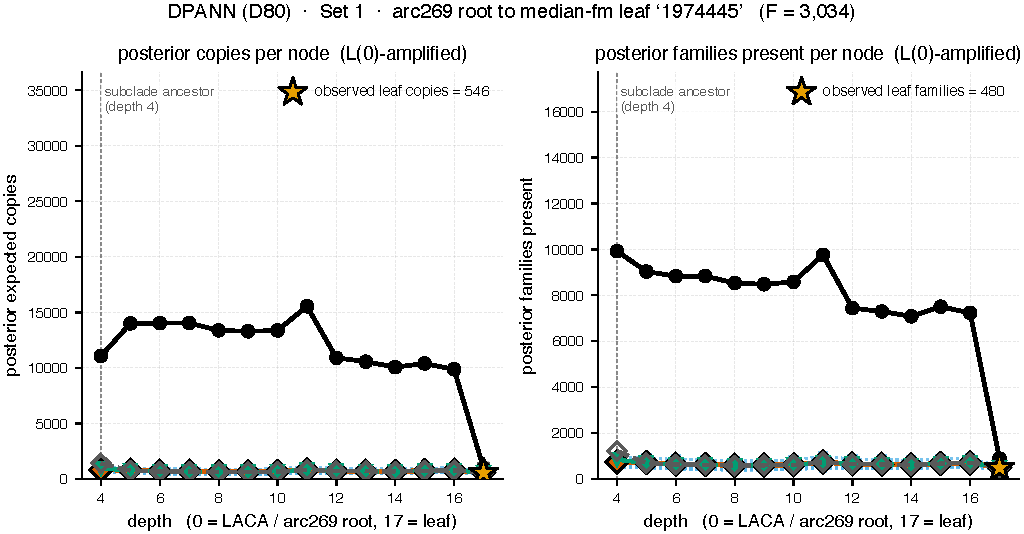
\includegraphics[width=0.92\linewidth,height=\textheight,keepaspectratio,alt={set 1 dpann80 L(0)-corrected}]{../validation/outputs/subset_min4_path_dpann80_l0corr.pdf}

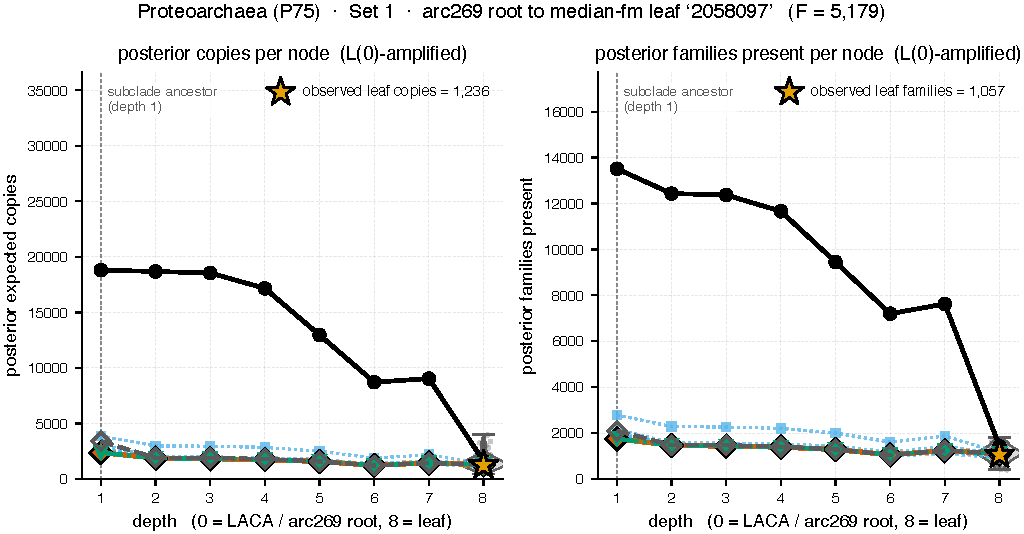
\includegraphics[width=0.92\linewidth,height=\textheight,keepaspectratio,alt={set 1 proteo75 L(0)-corrected}]{../validation/outputs/subset_min4_path_proteo75_l0corr.pdf}

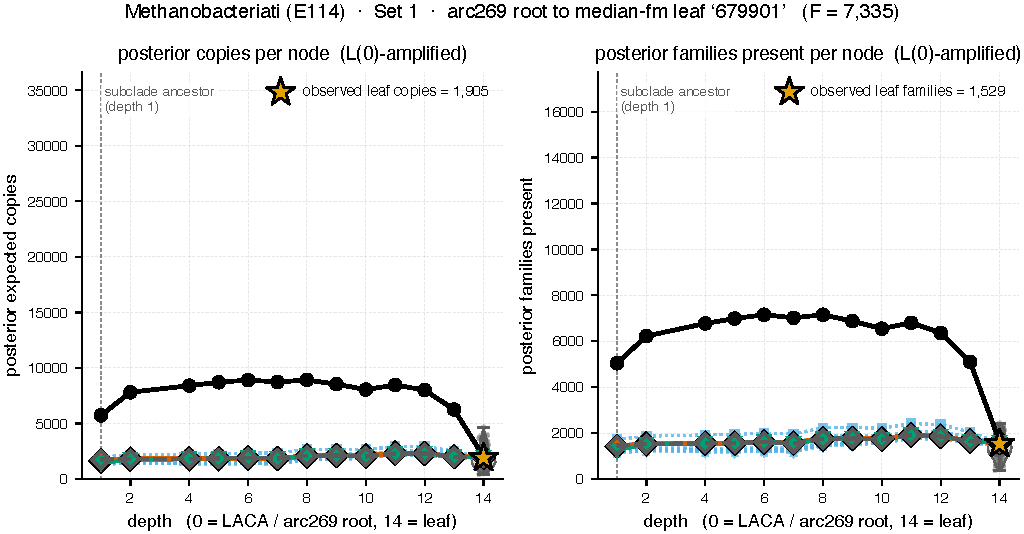
\includegraphics[width=0.92\linewidth,height=\textheight,keepaspectratio,alt={set 1 eury114 L(0)-corrected}]{../validation/outputs/subset_min4_path_eury114_l0corr.pdf}

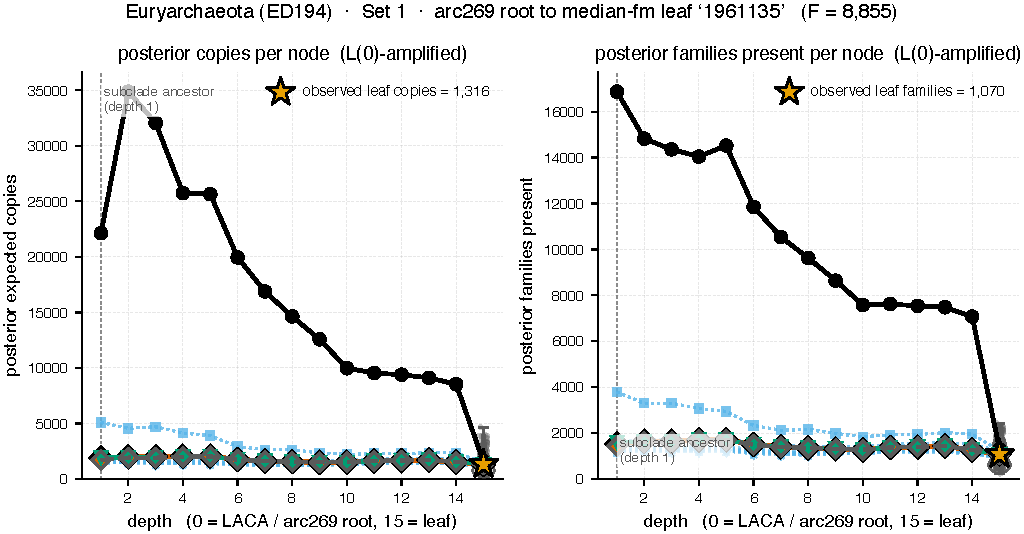
\includegraphics[width=0.92\linewidth,height=\textheight,keepaspectratio,alt={set 1 ed194 L(0)-corrected}]{../validation/outputs/subset_min4_path_ed194_l0corr.pdf}

\textbf{Figure 16.} Set 1 (per-clade sum-filter sweep) root-to-leaf
trajectories with the F* = F/(1−L(0)) amplification applied per line.

\subsubsection{Set 1.5 --- L(0)-corrected}\label{set-15--l0-corrected}

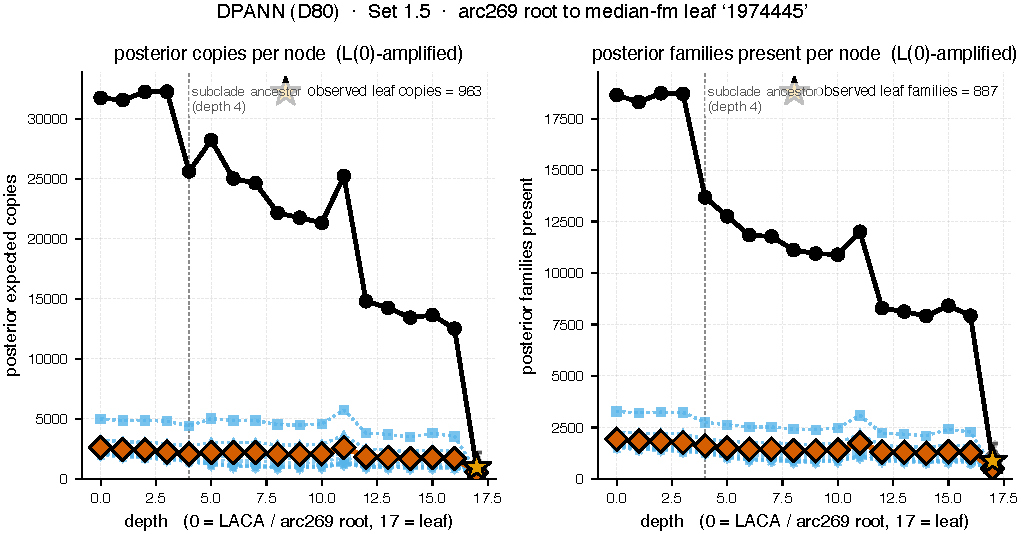
\includegraphics[width=0.92\linewidth,height=\textheight,keepaspectratio,alt={set 1.5 dpann80 L(0)-corrected}]{../validation/outputs/arc269_sumsweep_path_dpann80_l0corr.pdf}

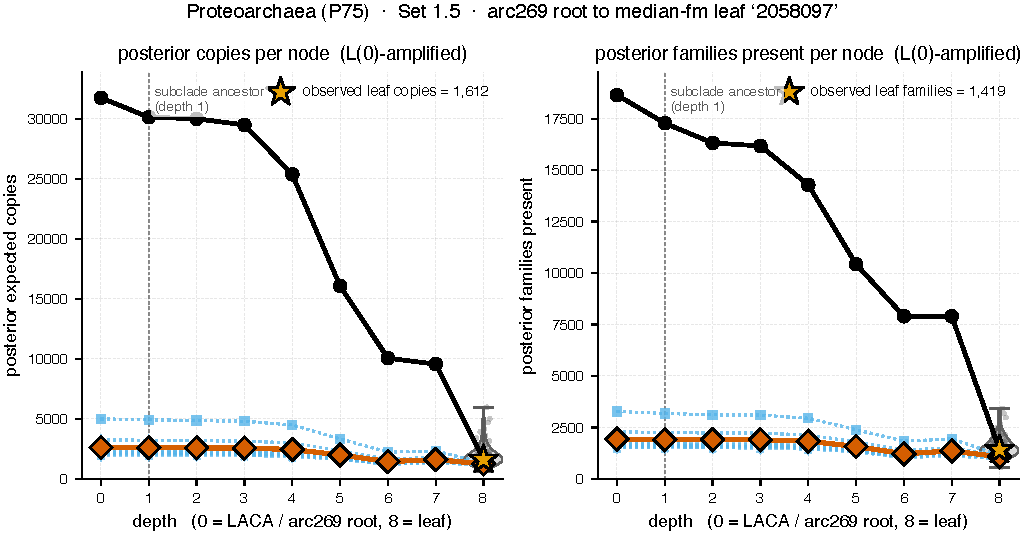
\includegraphics[width=0.92\linewidth,height=\textheight,keepaspectratio,alt={set 1.5 proteo75 L(0)-corrected}]{../validation/outputs/arc269_sumsweep_path_proteo75_l0corr.pdf}

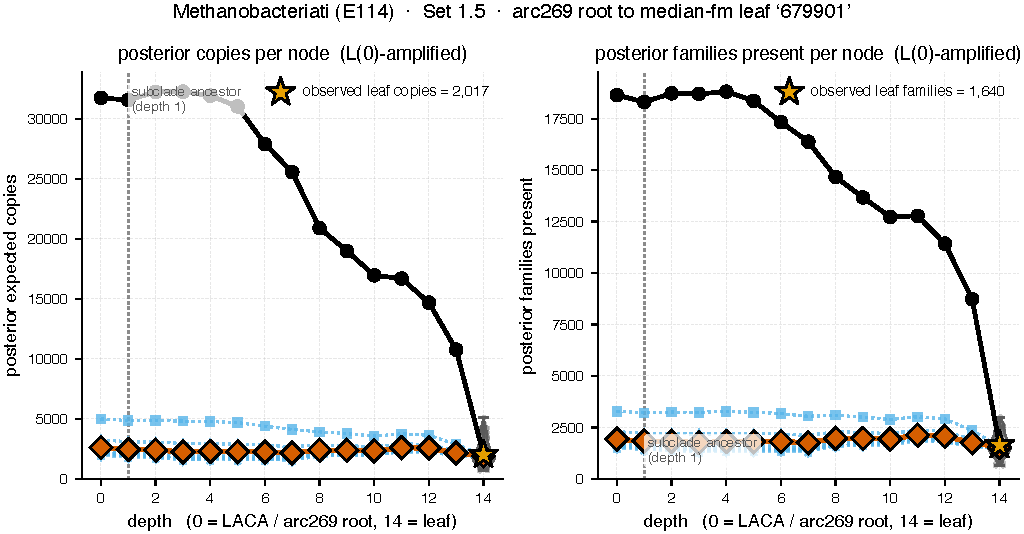
\includegraphics[width=0.92\linewidth,height=\textheight,keepaspectratio,alt={set 1.5 eury114 L(0)-corrected}]{../validation/outputs/arc269_sumsweep_path_eury114_l0corr.pdf}

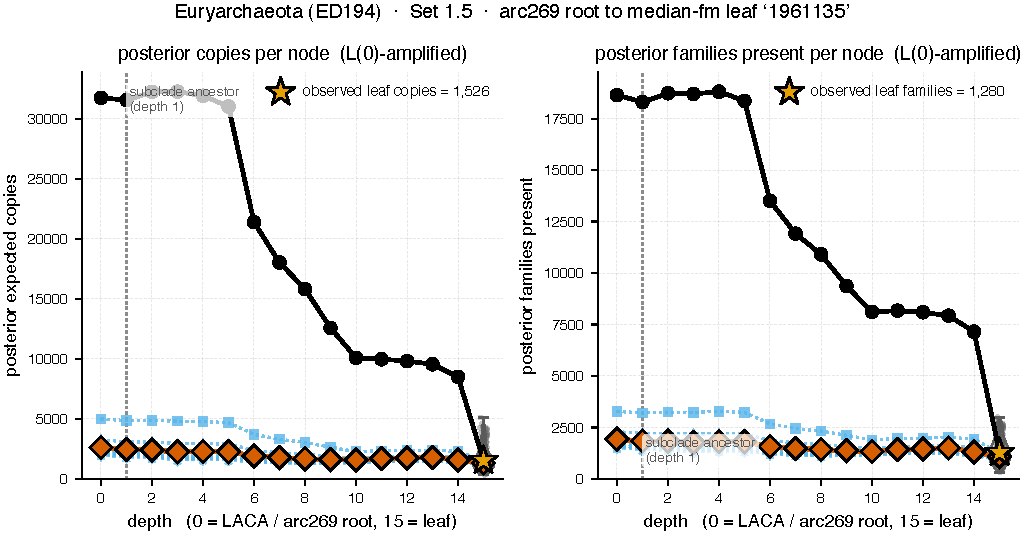
\includegraphics[width=0.92\linewidth,height=\textheight,keepaspectratio,alt={set 1.5 ed194 L(0)-corrected}]{../validation/outputs/arc269_sumsweep_path_ed194_l0corr.pdf}

\textbf{Figure 17.} Set 1.5 (arc269 full-tree sum-filter sweep)
root-to-leaf trajectories with the F* = F/(1−L(0)) amplification applied
per line.

\subsubsection{Set 2 --- L(0)-corrected}\label{set-2--l0-corrected}

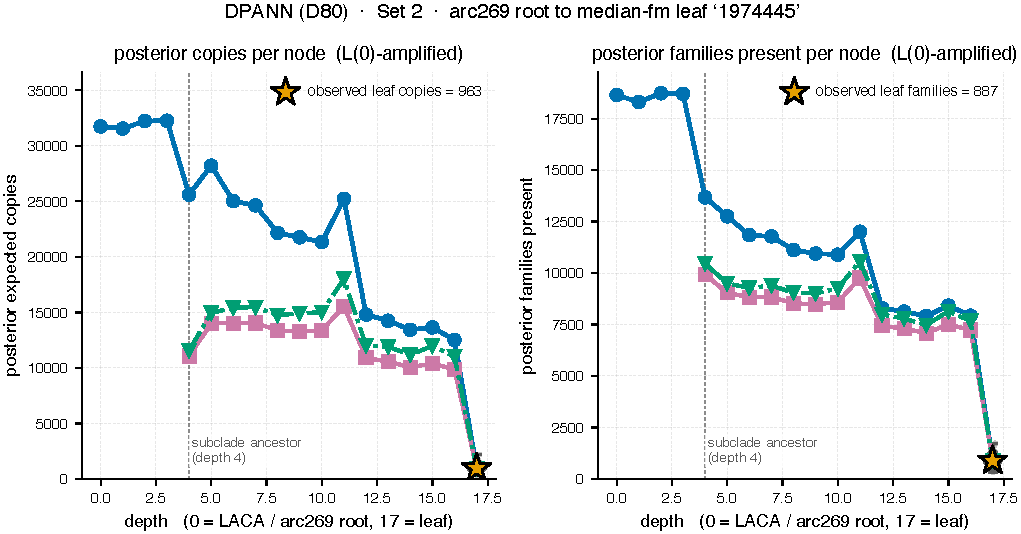
\includegraphics[width=0.92\linewidth,height=\textheight,keepaspectratio,alt={set 2 dpann80 L(0)-corrected}]{../validation/outputs/min1_path_dpann80_l0corr.pdf}

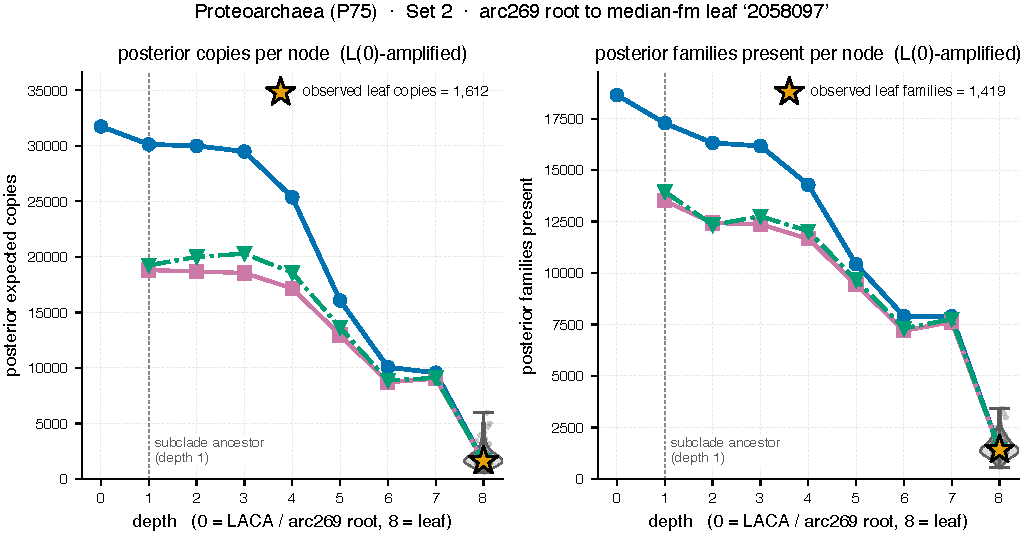
\includegraphics[width=0.92\linewidth,height=\textheight,keepaspectratio,alt={set 2 proteo75 L(0)-corrected}]{../validation/outputs/min1_path_proteo75_l0corr.pdf}

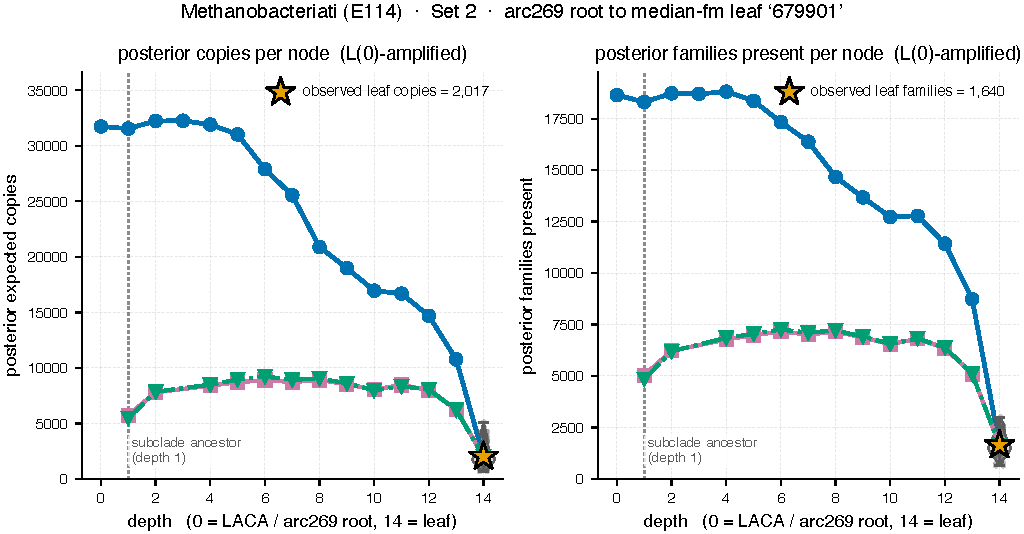
\includegraphics[width=0.92\linewidth,height=\textheight,keepaspectratio,alt={set 2 eury114 L(0)-corrected}]{../validation/outputs/min1_path_eury114_l0corr.pdf}

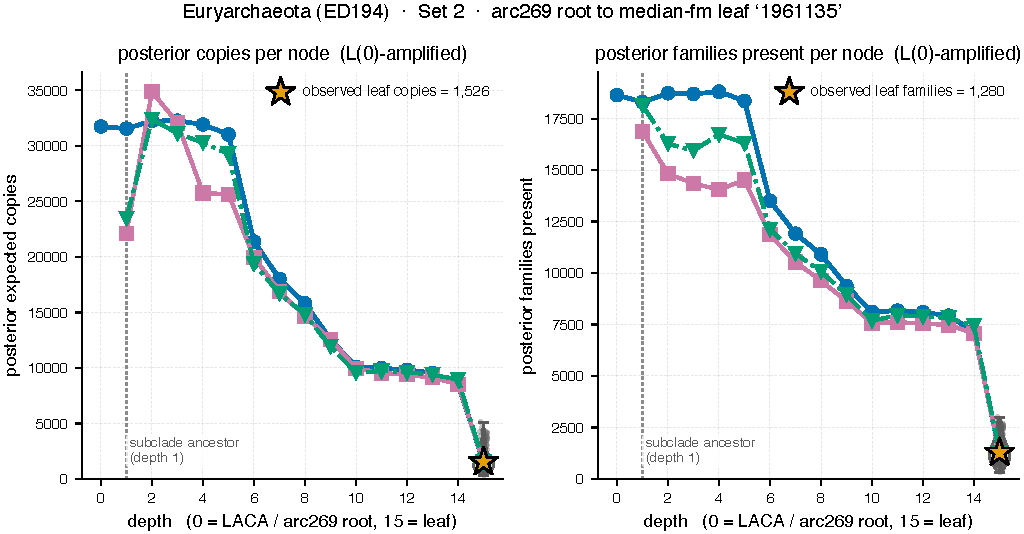
\includegraphics[width=0.92\linewidth,height=\textheight,keepaspectratio,alt={set 2 ed194 L(0)-corrected}]{../validation/outputs/min1_path_ed194_l0corr.pdf}

\textbf{Figure 18.} Set 2 (min = 1, no filter) root-to-leaf trajectories
with the F* = F/(1−L(0)) amplification applied per line.

\subsubsection{Set 3 --- L(0)-corrected}\label{set-3--l0-corrected}

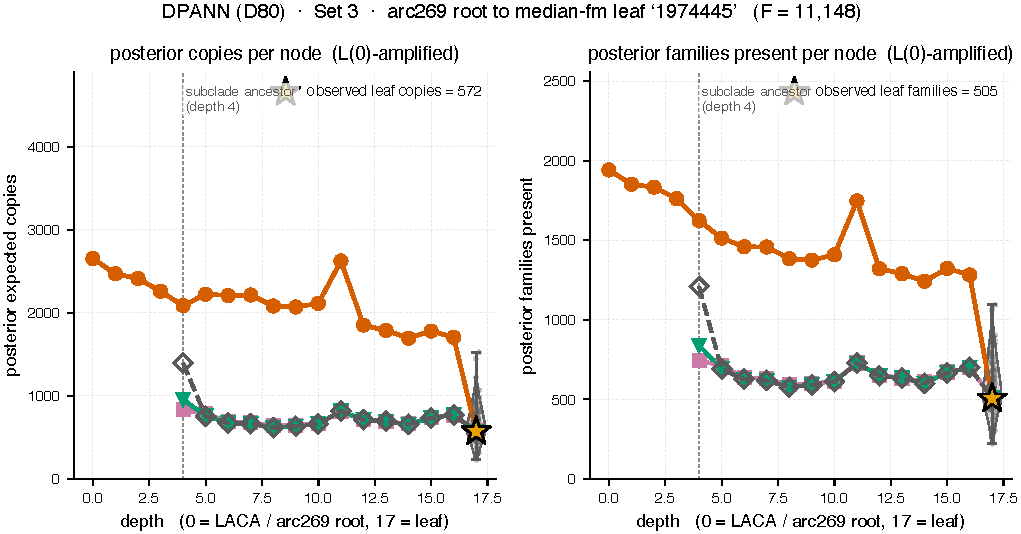
\includegraphics[width=0.92\linewidth,height=\textheight,keepaspectratio,alt={set 3 dpann80 L(0)-corrected}]{../validation/outputs/union_path_dpann80_l0corr.pdf}

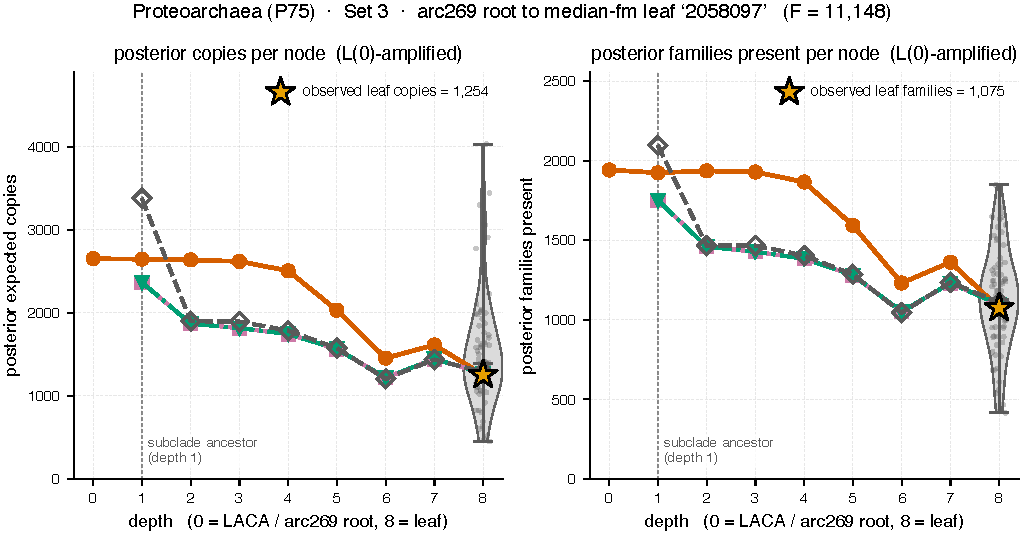
\includegraphics[width=0.92\linewidth,height=\textheight,keepaspectratio,alt={set 3 proteo75 L(0)-corrected}]{../validation/outputs/union_path_proteo75_l0corr.pdf}

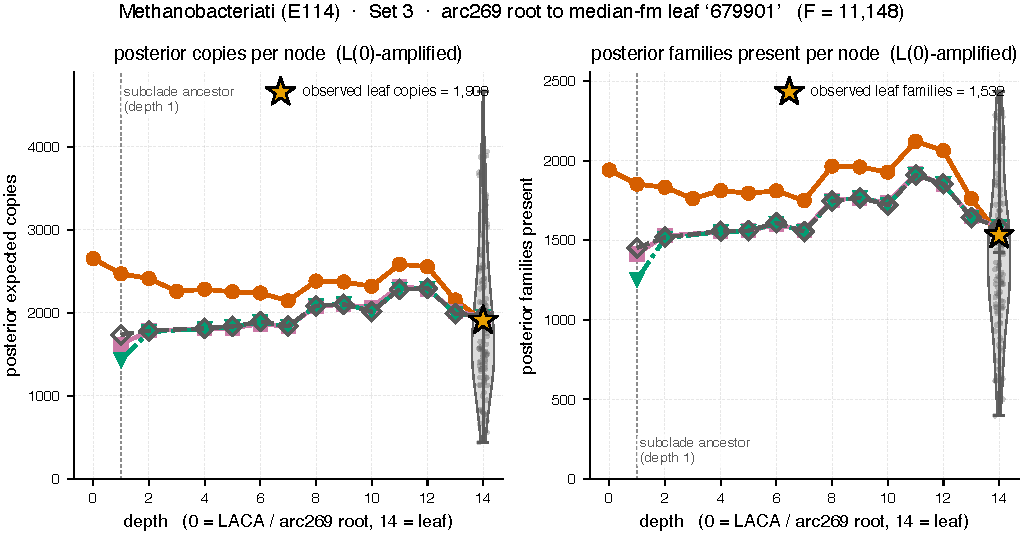
\includegraphics[width=0.92\linewidth,height=\textheight,keepaspectratio,alt={set 3 eury114 L(0)-corrected}]{../validation/outputs/union_path_eury114_l0corr.pdf}

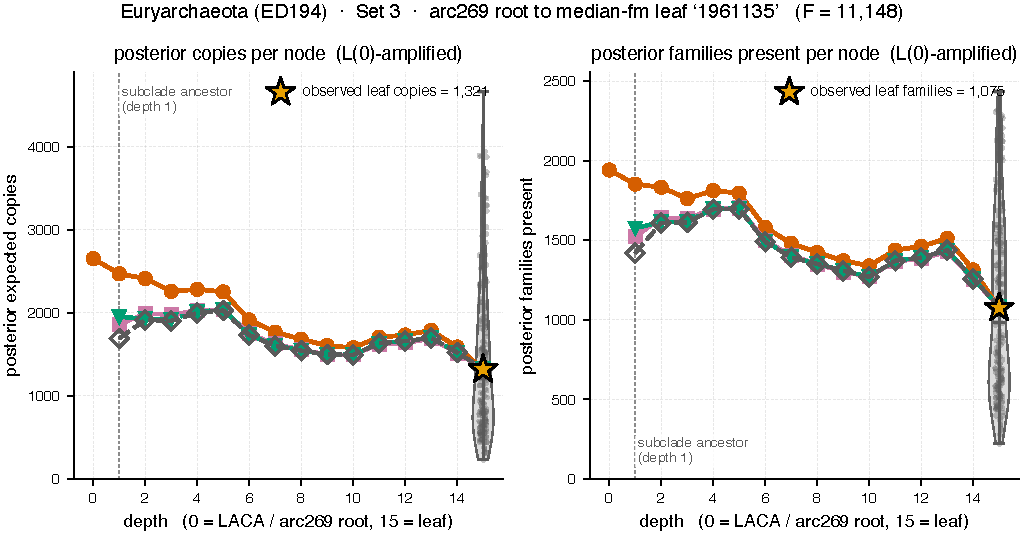
\includegraphics[width=0.92\linewidth,height=\textheight,keepaspectratio,alt={set 3 ed194 L(0)-corrected}]{../validation/outputs/union_path_ed194_l0corr.pdf}

\textbf{Figure 19.} Set 3 (arc269 full-tree fit on the union of
per-clade min = 4 families) root-to-leaf trajectories with the F* =
F/(1−L(0)) amplification applied per line.

\subsection{License}\label{license}

Apache License 2.0 --- see \url{LICENSE}. Same license as the original
Count Java package.

\end{document}
